%%%%%%%%%%%%%%%%%%%%%%%%%%%%%%%%%%%%%%%%%
% Masters/Doctoral Thesis
% LaTeX Template
% Version 2.5 (27/8/17)
%
% This template was downloaded from:
% http://www.LaTeXTemplates.com
%
% Version 2.x major modifications by:
% Vel (vel@latextemplates.com)
%
% This template is based on a template by:
% Steve Gunn (http://users.ecs.soton.ac.uk/srg/softwaretools/document/templates/)
% Sunil Patel (http://www.sunilpatel.co.uk/thesis-template/)
%
% Template license:
% CC BY-NC-SA 3.0 (http://creativecommons.org/licenses/by-nc-sa/3.0/)
%
%%%%%%%%%%%%%%%%%%%%%%%%%%%%%%%%%%%%%%%%%

%----------------------------------------------------------------------------------------
%	PACKAGES AND OTHER DOCUMENT CONFIGURATIONS
%----------------------------------------------------------------------------------------

\documentclass[
11pt, % The default document font size, options: 10pt, 11pt, 12pt
%oneside, % Two side (alternating margins) for binding by default, uncomment to switch to one side
english, % ngerman for German
singlespacing, % Single line spacing, alternatives: onehalfspacing or doublespacing
%draft, % Uncomment to enable draft mode (no pictures, no links, overfull hboxes indicated)
%nolistspacing, % If the document is onehalfspacing or doublespacing, uncomment this to set spacing in lists to single
%liststotoc, % Uncomment to add the list of figures/tables/etc to the table of contents
%toctotoc, % Uncomment to add the main table of contents to the table of contents
%parskip, % Uncomment to add space between paragraphs
%nohyperref, % Uncomment to not load the hyperref package
headsepline, % Uncomment to get a line under the header
%chapterinoneline, % Uncomment to place the chapter title next to the number on one line
%consistentlayout, % Uncomment to change the layout of the declaration, abstract and acknowledgements pages to match the default layout
]{MastersDoctoralThesis} % The class file specifying the document structure

\usepackage[utf8]{inputenc} % Required for inputting international characters
\usepackage[T1]{fontenc} % Output font encoding for international characters

\usepackage{mathpazo} % Use the Palatino font by default

% \usepackage[backend=bibtex,style=authoryear,natbib=true]{biblatex} % Use the bibtex backend with the authoryear citation style (which resembles APA)
\usepackage[backend=bibtex,style=numeric,natbib=true]{biblatex} % Use the bibtex backend with the authoryear citation style (which resembles APA)

\addbibresource{example.bib} % The filename of the bibliography
\addbibresource{ribes19bib.bib}
\addbibresource{other_references.bib}

\usepackage[autostyle=true]{csquotes} % Required to generate language-dependent quotes in the bibliography

\usepackage{mystyle}

%----------------------------------------------------------------------------------------
%	MARGIN SETTINGS
%----------------------------------------------------------------------------------------

\geometry{
	paper=a4paper, % Change to letterpaper for US letter
	inner=2.5cm, % Inner margin
	outer=3.8cm, % Outer margin
	bindingoffset=.5cm, % Binding offset
	top=1.5cm, % Top margin
	bottom=1.5cm, % Bottom margin
	%showframe, % Uncomment to show how the type block is set on the page
}

%----------------------------------------------------------------------------------------
%	THESIS INFORMATION
%----------------------------------------------------------------------------------------

\thesistitle{Using Random Fourier Features with Random Forest} % Your thesis title, this is used in the title and abstract, print it elsewhere with \ttitle
\supervisor{Lluís A. \textsc{Belanche}} % Your supervisor's name, this is used in the title page, print it elsewhere with \supname
\examiner{} % Your examiner's name, this is not currently used anywhere in the template, print it elsewhere with \examname
\degree{Bachelor Degree in Computer Science} % Your degree name, this is used in the title page and abstract, print it elsewhere with \degreename
\author{Albert \textsc{Ribes}} % Your name, this is used in the title page and abstract, print it elsewhere with \authorname
\addresses{} % Your address, this is not currently used anywhere in the template, print it elsewhere with \addressname

% \subject{Computing} % Your subject area, this is not currently used anywhere in the template, print it elsewhere with \subjectname
\subject{Major in Computing}
\keywords{} % Keywords for your thesis, this is not currently used anywhere in the template, print it elsewhere with \keywordnames
\university{\href{https://www.upc.edu/ca}{Universitat Politècnica de Catalunya (UPC) -- BarcelonaTech}} % Your university's name and URL, this is used in the title page and abstract, print it elsewhere with \univname
\department{\href{https://www.fib.upc.edu/en/research/departments/computer-science}{Computer Science}} % Your department's name and URL, this is used in the title page and abstract, print it elsewhere with \deptname
% \group{\href{http://researchgroup.university.com}{Research Group Name}} % Your research group's name and URL, this is used in the title page, print it elsewhere with \groupname
\faculty{\href{https://www.fib.upc.edu}{Facultat d’Informàtica de Barcelona (FIB)}} % Your faculty's name and URL, this is used in the title page and abstract, print it elsewhere with \facname

\AtBeginDocument{
\hypersetup{pdftitle=\ttitle} % Set the PDF's title to your title
\hypersetup{pdfauthor=\authorname} % Set the PDF's author to your name
\hypersetup{pdfkeywords=\keywordnames} % Set the PDF's keywords to your keywords
}

\begin{document}

\frontmatter % Use roman page numbering style (i, ii, iii, iv...) for the pre-content pages

\pagestyle{plain} % Default to the plain heading style until the thesis style is called for the body content

%----------------------------------------------------------------------------------------
%	TITLE PAGE
%----------------------------------------------------------------------------------------

\begin{titlepage}
\begin{center}

\vspace*{.06\textheight}
{\scshape\LARGE \univname\par}\vspace{1.5cm} % University name
% \textsc{\Large Doctoral Thesis}\\[0.5cm] % Thesis type
% \textsc{\Large Degree Final Project}\\[0.5cm] % Thesis type
\textsc{\Large Bachelor's Thesis}\\[0.5cm] % Thesis type

\HRule \\[0.4cm] % Horizontal line
{\huge \bfseries \ttitle\par}\vspace{0.4cm} % Thesis title
\HRule \\[1.5cm] % Horizontal line

\begin{minipage}[t]{0.4\textwidth}
\begin{flushleft} \large
\emph{Author:}\\
\authorname % Author name - remove the \href bracket to remove the link
\end{flushleft}
\end{minipage}
\begin{minipage}[t]{0.4\textwidth}
\begin{flushright} \large
\emph{Supervisor:} \\
\href{https://www.cs.upc.edu/~belanche/}{\supname} % Supervisor name - remove the \href bracket to remove the link
\end{flushright}
\end{minipage}\\[3cm]

\vfill

% \large \textit{A thesis submitted in fulfillment of the requirements\\ for the degree of \degreename}\\[0.3cm] % University requirement text
% \textit{in the}\\[0.4cm]
% \groupname\\\deptname\\[2cm] % Research group name and department name
\deptname\\[2cm] % Research group name and department name

\vfill

{\large \today}\\[4cm] % Date
%\includegraphics{Logo} % University/department logo - uncomment to place it

\vfill
\end{center}
\end{titlepage}

%----------------------------------------------------------------------------------------
%	DECLARATION PAGE
%----------------------------------------------------------------------------------------

% \begin{declaration}
% \addchaptertocentry{\authorshipname} % Add the declaration to the table of contents
% \noindent I, \authorname, declare that this thesis titled, \enquote{\ttitle} and the work presented in it are my own. I confirm that:
%
% \begin{itemize}
% \item This work was done wholly or mainly while in candidature for a research degree at this University.
% \item Where any part of this thesis has previously been submitted for a degree or any other qualification at this University or any other institution, this has been clearly stated.
% \item Where I have consulted the published work of others, this is always clearly attributed.
% \item Where I have quoted from the work of others, the source is always given. With the exception of such quotations, this thesis is entirely my own work.
% \item I have acknowledged all main sources of help.
% \item Where the thesis is based on work done by myself jointly with others, I have made clear exactly what was done by others and what I have contributed myself.\\
% \end{itemize}
%
% \noindent Signed:\\
% \rule[0.5em]{25em}{0.5pt} % This prints a line for the signature
%
% \noindent Date:\\
% \rule[0.5em]{25em}{0.5pt} % This prints a line to write the date
% \end{declaration}

\cleardoublepage

%----------------------------------------------------------------------------------------
%	QUOTATION PAGE
%----------------------------------------------------------------------------------------

% \vspace*{0.2\textheight}
%
% \noindent\enquote{\itshape Thanks to my solid academic training, today I can write hundreds of words on virtually any topic without possessing a shred of information, which is how I got a good job in journalism.}\bigbreak
%
% \hfill Dave Barry

%----------------------------------------------------------------------------------------
%	ABSTRACT PAGE
%----------------------------------------------------------------------------------------

\begin{abstract}
\addchaptertocentry{\abstractname} % Add the abstract to the table of contents
\begin{note}
	The Thesis Abstract is written here (and usually kept to just this page). The page is kept centered vertically so can expand into the blank space above the title too\ldots
	\begin{itemize}
		\item En 3 idiomas
	\end{itemize}
\end{note}
\end{abstract}



%----------------------------------------------------------------------------------------
%	ACKNOWLEDGEMENTS
%----------------------------------------------------------------------------------------

% \begin{acknowledgements}
% \addchaptertocentry{\acknowledgementname} % Add the acknowledgements to the table of contents
% The acknowledgments and the people to thank go here, don't forget to include your project advisor\ldots
% \end{acknowledgements}

%----------------------------------------------------------------------------------------
%	LIST OF CONTENTS/FIGURES/TABLES PAGES
%----------------------------------------------------------------------------------------

\tableofcontents % Prints the main table of contents

% \listoffigures % Prints the list of figures

% \listoftables % Prints the list of tables

%----------------------------------------------------------------------------------------
%	ABBREVIATIONS
%----------------------------------------------------------------------------------------

% \begin{abbreviations}{ll} % Include a list of abbreviations (a table of two columns)
%
% \textbf{ML} & \textbf{M}achine \textbf{L}earning\\
% \textbf{SVM} & \textbf{S}upport \textbf{V}ector \textbf{M}achine\\
% \textbf{RBF} & \textbf{R}adial \textbf{B}asis \textbf{F}unction\\
% \textbf{DT} & \textbf{D}ecision \textbf{T}ree\\
% \textbf{RF} & \textbf{R}andom \textbf{F}orest\\
% \textbf{RFF} & \textbf{R}andom \textbf{F}ourier \textbf{F}eatures\\
% \textbf{CV} & \textbf{C}ross-\textbf{V}alidation\\
%
%
% \end{abbreviations}

%----------------------------------------------------------------------------------------
%	PHYSICAL CONSTANTS/OTHER DEFINITIONS
%----------------------------------------------------------------------------------------

% \begin{constants}{lr@{${}={}$}l} % The list of physical constants is a three column table
%
% % The \SI{}{} command is provided by the siunitx package, see its documentation for instructions on how to use it
%
% Speed of Light & $c_{0}$ & \SI{2.99792458e8}{\meter\per\second} (exact)\\
% %Constant Name & $Symbol$ & $Constant Value$ with units\\
%
% \end{constants}

%----------------------------------------------------------------------------------------
%	SYMBOLS
%----------------------------------------------------------------------------------------

% \begin{symbols}{lll} % Include a list of Symbols (a three column table)
%
% $a$ & distance & \si{\meter} \\
% $P$ & power & \si{\watt} (\si{\joule\per\second}) \\
% %Symbol & Name & Unit \\
%
% \addlinespace % Gap to separate the Roman symbols from the Greek
%
% $\omega$ & angular frequency & \si{\radian} \\
%
% \end{symbols}

%----------------------------------------------------------------------------------------
%	DEDICATION
%----------------------------------------------------------------------------------------

% \dedicatory{For/Dedicated to/To my\ldots}

%----------------------------------------------------------------------------------------
%	THESIS CONTENT - CHAPTERS
%----------------------------------------------------------------------------------------

\mainmatter % Begin numeric (1,2,3...) page numbering

\pagestyle{thesis} % Return the page headers back to the "thesis" style

% Include the chapters of the thesis as separate files from the Chapters folder
% Uncomment the lines as you write the chapters

% % Chapter 1

\chapter{Chapter Title Here} % Main chapter title

\label{Chapter1} % For referencing the chapter elsewhere, use \ref{Chapter1}

%----------------------------------------------------------------------------------------

% Define some commands to keep the formatting separated from the content
\newcommand{\keyword}[1]{\textbf{#1}}
\newcommand{\tabhead}[1]{\textbf{#1}}
\newcommand{\code}[1]{\texttt{#1}}
\newcommand{\file}[1]{\texttt{\bfseries#1}}
\newcommand{\option}[1]{\texttt{\itshape#1}}

%----------------------------------------------------------------------------------------

\section{Welcome and Thank You}
Welcome to this \LaTeX{} Thesis Template, a beautiful and easy to use template for writing a thesis using the \LaTeX{} typesetting system.

If you are writing a thesis (or will be in the future) and its subject is technical or mathematical (though it doesn't have to be), then creating it in \LaTeX{} is highly recommended as a way to make sure you can just get down to the essential writing without having to worry over formatting or wasting time arguing with your word processor.

\LaTeX{} is easily able to professionally typeset documents that run to hundreds or thousands of pages long. With simple mark-up commands, it automatically sets out the table of contents, margins, page headers and footers and keeps the formatting consistent and beautiful. One of its main strengths is the way it can easily typeset mathematics, even \emph{heavy} mathematics. Even if those equations are the most horribly twisted and most difficult mathematical problems that can only be solved on a super-computer, you can at least count on \LaTeX{} to make them look stunning.

%----------------------------------------------------------------------------------------

\section{Learning \LaTeX{}}

\LaTeX{} is not a \textsc{wysiwyg} (What You See is What You Get) program, unlike word processors such as Microsoft Word or Apple's Pages. Instead, a document written for \LaTeX{} is actually a simple, plain text file that contains \emph{no formatting}. You tell \LaTeX{} how you want the formatting in the finished document by writing in simple commands amongst the text, for example, if I want to use \emph{italic text for emphasis}, I write the \verb|\emph{text}| command and put the text I want in italics in between the curly braces. This means that \LaTeX{} is a \enquote{mark-up} language, very much like HTML.

\subsection{A (not so short) Introduction to \LaTeX{}}

If you are new to \LaTeX{}, there is a very good eBook -- freely available online as a PDF file -- called, \enquote{The Not So Short Introduction to \LaTeX{}}. The book's title is typically shortened to just \emph{lshort}. You can download the latest version (as it is occasionally updated) from here:
\url{http://www.ctan.org/tex-archive/info/lshort/english/lshort.pdf}

It is also available in several other languages. Find yours from the list on this page: \url{http://www.ctan.org/tex-archive/info/lshort/}

It is recommended to take a little time out to learn how to use \LaTeX{} by creating several, small `test' documents, or having a close look at several templates on:\\
\url{http://www.LaTeXTemplates.com}\\
Making the effort now means you're not stuck learning the system when what you \emph{really} need to be doing is writing your thesis.

\subsection{A Short Math Guide for \LaTeX{}}

If you are writing a technical or mathematical thesis, then you may want to read the document by the AMS (American Mathematical Society) called, \enquote{A Short Math Guide for \LaTeX{}}. It can be found online here:
\url{http://www.ams.org/tex/amslatex.html}
under the \enquote{Additional Documentation} section towards the bottom of the page.

\subsection{Common \LaTeX{} Math Symbols}
There are a multitude of mathematical symbols available for \LaTeX{} and it would take a great effort to learn the commands for them all. The most common ones you are likely to use are shown on this page:
\url{http://www.sunilpatel.co.uk/latex-type/latex-math-symbols/}

You can use this page as a reference or crib sheet, the symbols are rendered as large, high quality images so you can quickly find the \LaTeX{} command for the symbol you need.

\subsection{\LaTeX{} on a Mac}

The \LaTeX{} distribution is available for many systems including Windows, Linux and Mac OS X. The package for OS X is called MacTeX and it contains all the applications you need -- bundled together and pre-customized -- for a fully working \LaTeX{} environment and work flow.

MacTeX includes a custom dedicated \LaTeX{} editor called TeXShop for writing your `\file{.tex}' files and BibDesk: a program to manage your references and create your bibliography section just as easily as managing songs and creating playlists in iTunes.

%----------------------------------------------------------------------------------------

\section{Getting Started with this Template}

If you are familiar with \LaTeX{}, then you should explore the directory structure of the template and then proceed to place your own information into the \emph{THESIS INFORMATION} block of the \file{main.tex} file. You can then modify the rest of this file to your unique specifications based on your degree/university. Section \ref{FillingFile} on page \pageref{FillingFile} will help you do this. Make sure you also read section \ref{ThesisConventions} about thesis conventions to get the most out of this template.

If you are new to \LaTeX{} it is recommended that you carry on reading through the rest of the information in this document.

Before you begin using this template you should ensure that its style complies with the thesis style guidelines imposed by your institution. In most cases this template style and layout will be suitable. If it is not, it may only require a small change to bring the template in line with your institution's recommendations. These modifications will need to be done on the \file{MastersDoctoralThesis.cls} file.

\subsection{About this Template}

This \LaTeX{} Thesis Template is originally based and created around a \LaTeX{} style file created by Steve R.\ Gunn from the University of Southampton (UK), department of Electronics and Computer Science. You can find his original thesis style file at his site, here:
\url{http://www.ecs.soton.ac.uk/~srg/softwaretools/document/templates/}

Steve's \file{ecsthesis.cls} was then taken by Sunil Patel who modified it by creating a skeleton framework and folder structure to place the thesis files in. The resulting template can be found on Sunil's site here:
\url{http://www.sunilpatel.co.uk/thesis-template}

Sunil's template was made available through \url{http://www.LaTeXTemplates.com} where it was modified many times based on user requests and questions. Version 2.0 and onwards of this template represents a major modification to Sunil's template and is, in fact, hardly recognisable. The work to make version 2.0 possible was carried out by \href{mailto:vel@latextemplates.com}{Vel} and Johannes Böttcher.

%----------------------------------------------------------------------------------------

\section{What this Template Includes}

\subsection{Folders}

This template comes as a single zip file that expands out to several files and folders. The folder names are mostly self-explanatory:

\keyword{Appendices} -- this is the folder where you put the appendices. Each appendix should go into its own separate \file{.tex} file. An example and template are included in the directory.

\keyword{Chapters} -- this is the folder where you put the thesis chapters. A thesis usually has about six chapters, though there is no hard rule on this. Each chapter should go in its own separate \file{.tex} file and they can be split as:
\begin{itemize}
\item Chapter 1: Introduction to the thesis topic
\item Chapter 2: Background information and theory
\item Chapter 3: (Laboratory) experimental setup
\item Chapter 4: Details of experiment 1
\item Chapter 5: Details of experiment 2
\item Chapter 6: Discussion of the experimental results
\item Chapter 7: Conclusion and future directions
\end{itemize}
This chapter layout is specialised for the experimental sciences, your discipline may be different.

\keyword{Figures} -- this folder contains all figures for the thesis. These are the final images that will go into the thesis document.

\subsection{Files}

Included are also several files, most of them are plain text and you can see their contents in a text editor. After initial compilation, you will see that more auxiliary files are created by \LaTeX{} or BibTeX and which you don't need to delete or worry about:

\keyword{example.bib} -- this is an important file that contains all the bibliographic information and references that you will be citing in the thesis for use with BibTeX. You can write it manually, but there are reference manager programs available that will create and manage it for you. Bibliographies in \LaTeX{} are a large subject and you may need to read about BibTeX before starting with this. Many modern reference managers will allow you to export your references in BibTeX format which greatly eases the amount of work you have to do.

\keyword{MastersDoctoralThesis.cls} -- this is an important file. It is the class file that tells \LaTeX{} how to format the thesis.

\keyword{main.pdf} -- this is your beautifully typeset thesis (in the PDF file format) created by \LaTeX{}. It is supplied in the PDF with the template and after you compile the template you should get an identical version.

\keyword{main.tex} -- this is an important file. This is the file that you tell \LaTeX{} to compile to produce your thesis as a PDF file. It contains the framework and constructs that tell \LaTeX{} how to layout the thesis. It is heavily commented so you can read exactly what each line of code does and why it is there. After you put your own information into the \emph{THESIS INFORMATION} block -- you have now started your thesis!

Files that are \emph{not} included, but are created by \LaTeX{} as auxiliary files include:

\keyword{main.aux} -- this is an auxiliary file generated by \LaTeX{}, if it is deleted \LaTeX{} simply regenerates it when you run the main \file{.tex} file.

\keyword{main.bbl} -- this is an auxiliary file generated by BibTeX, if it is deleted, BibTeX simply regenerates it when you run the \file{main.aux} file. Whereas the \file{.bib} file contains all the references you have, this \file{.bbl} file contains the references you have actually cited in the thesis and is used to build the bibliography section of the thesis.

\keyword{main.blg} -- this is an auxiliary file generated by BibTeX, if it is deleted BibTeX simply regenerates it when you run the main \file{.aux} file.

\keyword{main.lof} -- this is an auxiliary file generated by \LaTeX{}, if it is deleted \LaTeX{} simply regenerates it when you run the main \file{.tex} file. It tells \LaTeX{} how to build the \emph{List of Figures} section.

\keyword{main.log} -- this is an auxiliary file generated by \LaTeX{}, if it is deleted \LaTeX{} simply regenerates it when you run the main \file{.tex} file. It contains messages from \LaTeX{}, if you receive errors and warnings from \LaTeX{}, they will be in this \file{.log} file.

\keyword{main.lot} -- this is an auxiliary file generated by \LaTeX{}, if it is deleted \LaTeX{} simply regenerates it when you run the main \file{.tex} file. It tells \LaTeX{} how to build the \emph{List of Tables} section.

\keyword{main.out} -- this is an auxiliary file generated by \LaTeX{}, if it is deleted \LaTeX{} simply regenerates it when you run the main \file{.tex} file.

So from this long list, only the files with the \file{.bib}, \file{.cls} and \file{.tex} extensions are the most important ones. The other auxiliary files can be ignored or deleted as \LaTeX{} and BibTeX will regenerate them.

%----------------------------------------------------------------------------------------

\section{Filling in Your Information in the \file{main.tex} File}\label{FillingFile}

You will need to personalise the thesis template and make it your own by filling in your own information. This is done by editing the \file{main.tex} file in a text editor or your favourite LaTeX environment.

Open the file and scroll down to the third large block titled \emph{THESIS INFORMATION} where you can see the entries for \emph{University Name}, \emph{Department Name}, etc \ldots

Fill out the information about yourself, your group and institution. You can also insert web links, if you do, make sure you use the full URL, including the \code{http://} for this. If you don't want these to be linked, simply remove the \verb|\href{url}{name}| and only leave the name.

When you have done this, save the file and recompile \code{main.tex}. All the information you filled in should now be in the PDF, complete with web links. You can now begin your thesis proper!

%----------------------------------------------------------------------------------------

\section{The \code{main.tex} File Explained}

The \file{main.tex} file contains the structure of the thesis. There are plenty of written comments that explain what pages, sections and formatting the \LaTeX{} code is creating. Each major document element is divided into commented blocks with titles in all capitals to make it obvious what the following bit of code is doing. Initially there seems to be a lot of \LaTeX{} code, but this is all formatting, and it has all been taken care of so you don't have to do it.

Begin by checking that your information on the title page is correct. For the thesis declaration, your institution may insist on something different than the text given. If this is the case, just replace what you see with what is required in the \emph{DECLARATION PAGE} block.

Then comes a page which contains a funny quote. You can put your own, or quote your favourite scientist, author, person, and so on. Make sure to put the name of the person who you took the quote from.

Following this is the abstract page which summarises your work in a condensed way and can almost be used as a standalone document to describe what you have done. The text you write will cause the heading to move up so don't worry about running out of space.

Next come the acknowledgements. On this page, write about all the people who you wish to thank (not forgetting parents, partners and your advisor/supervisor).

The contents pages, list of figures and tables are all taken care of for you and do not need to be manually created or edited. The next set of pages are more likely to be optional and can be deleted since they are for a more technical thesis: insert a list of abbreviations you have used in the thesis, then a list of the physical constants and numbers you refer to and finally, a list of mathematical symbols used in any formulae. Making the effort to fill these tables means the reader has a one-stop place to refer to instead of searching the internet and references to try and find out what you meant by certain abbreviations or symbols.

The list of symbols is split into the Roman and Greek alphabets. Whereas the abbreviations and symbols ought to be listed in alphabetical order (and this is \emph{not} done automatically for you) the list of physical constants should be grouped into similar themes.

The next page contains a one line dedication. Who will you dedicate your thesis to?

Finally, there is the block where the chapters are included. Uncomment the lines (delete the \code{\%} character) as you write the chapters. Each chapter should be written in its own file and put into the \emph{Chapters} folder and named \file{Chapter1}, \file{Chapter2}, etc\ldots Similarly for the appendices, uncomment the lines as you need them. Each appendix should go into its own file and placed in the \emph{Appendices} folder.

After the preamble, chapters and appendices finally comes the bibliography. The bibliography style (called \option{authoryear}) is used for the bibliography and is a fully featured style that will even include links to where the referenced paper can be found online. Do not underestimate how grateful your reader will be to find that a reference to a paper is just a click away. Of course, this relies on you putting the URL information into the BibTeX file in the first place.

%----------------------------------------------------------------------------------------

\section{Thesis Features and Conventions}\label{ThesisConventions}

To get the best out of this template, there are a few conventions that you may want to follow.

One of the most important (and most difficult) things to keep track of in such a long document as a thesis is consistency. Using certain conventions and ways of doing things (such as using a Todo list) makes the job easier. Of course, all of these are optional and you can adopt your own method.

\subsection{Printing Format}

This thesis template is designed for double sided printing (i.e. content on the front and back of pages) as most theses are printed and bound this way. Switching to one sided printing is as simple as uncommenting the \option{oneside} option of the \code{documentclass} command at the top of the \file{main.tex} file. You may then wish to adjust the margins to suit specifications from your institution.

The headers for the pages contain the page number on the outer side (so it is easy to flick through to the page you want) and the chapter name on the inner side.

The text is set to 11 point by default with single line spacing, again, you can tune the text size and spacing should you want or need to using the options at the very start of \file{main.tex}. The spacing can be changed similarly by replacing the \option{singlespacing} with \option{onehalfspacing} or \option{doublespacing}.

\subsection{Using US Letter Paper}

The paper size used in the template is A4, which is the standard size in Europe. If you are using this thesis template elsewhere and particularly in the United States, then you may have to change the A4 paper size to the US Letter size. This can be done in the margins settings section in \file{main.tex}.

Due to the differences in the paper size, the resulting margins may be different to what you like or require (as it is common for institutions to dictate certain margin sizes). If this is the case, then the margin sizes can be tweaked by modifying the values in the same block as where you set the paper size. Now your document should be set up for US Letter paper size with suitable margins.

\subsection{References}

The \code{biblatex} package is used to format the bibliography and inserts references such as this one \parencite{Reference1}. The options used in the \file{main.tex} file mean that the in-text citations of references are formatted with the author(s) listed with the date of the publication. Multiple references are separated by semicolons (e.g. \parencite{Reference2, Reference1}) and references with more than three authors only show the first author with \emph{et al.} indicating there are more authors (e.g. \parencite{Reference3}). This is done automatically for you. To see how you use references, have a look at the \file{Chapter1.tex} source file. Many reference managers allow you to simply drag the reference into the document as you type.

Scientific references should come \emph{before} the punctuation mark if there is one (such as a comma or period). The same goes for footnotes\footnote{Such as this footnote, here down at the bottom of the page.}. You can change this but the most important thing is to keep the convention consistent throughout the thesis. Footnotes themselves should be full, descriptive sentences (beginning with a capital letter and ending with a full stop). The APA6 states: \enquote{Footnote numbers should be superscripted, [...], following any punctuation mark except a dash.} The Chicago manual of style states: \enquote{A note number should be placed at the end of a sentence or clause. The number follows any punctuation mark except the dash, which it precedes. It follows a closing parenthesis.}

The bibliography is typeset with references listed in alphabetical order by the first author's last name. This is similar to the APA referencing style. To see how \LaTeX{} typesets the bibliography, have a look at the very end of this document (or just click on the reference number links in in-text citations).

\subsubsection{A Note on bibtex}

The bibtex backend used in the template by default does not correctly handle unicode character encoding (i.e. "international" characters). You may see a warning about this in the compilation log and, if your references contain unicode characters, they may not show up correctly or at all. The solution to this is to use the biber backend instead of the outdated bibtex backend. This is done by finding this in \file{main.tex}: \option{backend=bibtex} and changing it to \option{backend=biber}. You will then need to delete all auxiliary BibTeX files and navigate to the template directory in your terminal (command prompt). Once there, simply type \code{biber main} and biber will compile your bibliography. You can then compile \file{main.tex} as normal and your bibliography will be updated. An alternative is to set up your LaTeX editor to compile with biber instead of bibtex, see \href{http://tex.stackexchange.com/questions/154751/biblatex-with-biber-configuring-my-editor-to-avoid-undefined-citations/}{here} for how to do this for various editors.

\subsection{Tables}

Tables are an important way of displaying your results, below is an example table which was generated with this code:

{\small
\begin{verbatim}
\begin{table}
\caption{The effects of treatments X and Y on the four groups studied.}
\label{tab:treatments}
\centering
\begin{tabular}{l l l}
\toprule
\tabhead{Groups} & \tabhead{Treatment X} & \tabhead{Treatment Y} \\
\midrule
1 & 0.2 & 0.8\\
2 & 0.17 & 0.7\\
3 & 0.24 & 0.75\\
4 & 0.68 & 0.3\\
\bottomrule\\
\end{tabular}
\end{table}
\end{verbatim}
}

\begin{table}
\caption{The effects of treatments X and Y on the four groups studied.}
\label{tab:treatments}
\centering
\begin{tabular}{l l l}
\toprule
\tabhead{Groups} & \tabhead{Treatment X} & \tabhead{Treatment Y} \\
\midrule
1 & 0.2 & 0.8\\
2 & 0.17 & 0.7\\
3 & 0.24 & 0.75\\
4 & 0.68 & 0.3\\
\bottomrule\\
\end{tabular}
\end{table}

You can reference tables with \verb|\ref{<label>}| where the label is defined within the table environment. See \file{Chapter1.tex} for an example of the label and citation (e.g. Table~\ref{tab:treatments}).

\subsection{Figures}

There will hopefully be many figures in your thesis (that should be placed in the \emph{Figures} folder). The way to insert figures into your thesis is to use a code template like this:
\begin{verbatim}
\begin{figure}
\centering

\includegraphics{Figures/Electron}
\decoRule
\caption[An Electron]{An electron (artist's impression).}
\label{fig:Electron}
\end{figure}
\end{verbatim}
Also look in the source file. Putting this code into the source file produces the picture of the electron that you can see in the figure below.

\begin{figure}[th]
\centering

\includegraphics{Figures/Electron}
\decoRule
\caption[An Electron]{An electron (artist's impression).}
\label{fig:Electron}
\end{figure}

Sometimes figures don't always appear where you write them in the source. The placement depends on how much space there is on the page for the figure. Sometimes there is not enough room to fit a figure directly where it should go (in relation to the text) and so \LaTeX{} puts it at the top of the next page. Positioning figures is the job of \LaTeX{} and so you should only worry about making them look good!

Figures usually should have captions just in case you need to refer to them (such as in Figure~\ref{fig:Electron}). The \verb|\caption| command contains two parts, the first part, inside the square brackets is the title that will appear in the \emph{List of Figures}, and so should be short. The second part in the curly brackets should contain the longer and more descriptive caption text.

The \verb|\decoRule| command is optional and simply puts an aesthetic horizontal line below the image. If you do this for one image, do it for all of them.

\LaTeX{} is capable of using images in pdf, jpg and png format.

\subsection{Typesetting mathematics}

If your thesis is going to contain heavy mathematical content, be sure that \LaTeX{} will make it look beautiful, even though it won't be able to solve the equations for you.

The \enquote{Not So Short Introduction to \LaTeX} (available on \href{http://www.ctan.org/tex-archive/info/lshort/english/lshort.pdf}{CTAN}) should tell you everything you need to know for most cases of typesetting mathematics. If you need more information, a much more thorough mathematical guide is available from the AMS called, \enquote{A Short Math Guide to \LaTeX} and can be downloaded from:
\url{ftp://ftp.ams.org/pub/tex/doc/amsmath/short-math-guide.pdf}

There are many different \LaTeX{} symbols to remember, luckily you can find the most common symbols in \href{http://ctan.org/pkg/comprehensive}{The Comprehensive \LaTeX~Symbol List}.

You can write an equation, which is automatically given an equation number by \LaTeX{} like this:
\begin{verbatim}
\begin{equation}
E = mc^{2}
\label{eqn:Einstein}
\end{equation}
\end{verbatim}

This will produce Einstein's famous energy-matter equivalence equation:
\begin{equation}
E = mc^{2}
\label{eqn:Einstein}
\end{equation}

All equations you write (which are not in the middle of paragraph text) are automatically given equation numbers by \LaTeX{}. If you don't want a particular equation numbered, use the unnumbered form:
\begin{verbatim}
\[ a^{2}=4 \]
\end{verbatim}

%----------------------------------------------------------------------------------------

\section{Sectioning and Subsectioning}

You should break your thesis up into nice, bite-sized sections and subsections. \LaTeX{} automatically builds a table of Contents by looking at all the \verb|\chapter{}|, \verb|\section{}|  and \verb|\subsection{}| commands you write in the source.

The Table of Contents should only list the sections to three (3) levels. A \verb|chapter{}| is level zero (0). A \verb|\section{}| is level one (1) and so a \verb|\subsection{}| is level two (2). In your thesis it is likely that you will even use a \verb|subsubsection{}|, which is level three (3). The depth to which the Table of Contents is formatted is set within \file{MastersDoctoralThesis.cls}. If you need this changed, you can do it in \file{main.tex}.

%----------------------------------------------------------------------------------------

\section{In Closing}

You have reached the end of this mini-guide. You can now rename or overwrite this pdf file and begin writing your own \file{Chapter1.tex} and the rest of your thesis. The easy work of setting up the structure and framework has been taken care of for you. It's now your job to fill it out!

Good luck and have lots of fun!

\begin{flushright}
Guide written by ---\\
Sunil Patel: \href{http://www.sunilpatel.co.uk}{www.sunilpatel.co.uk}\\
Vel: \href{http://www.LaTeXTemplates.com}{LaTeXTemplates.com}
\end{flushright}

%\include{Chapters/Chapter2}
%\include{Chapters/Chapter3}
%\include{Chapters/Chapter4}
%\include{Chapters/Chapter5}

% Chapter Template

\chapter{Introduction} % Main chapter title

\label{Chapter1} % Change X to a consecutive number; for referencing this chapter elsewhere, use \ref{ChapterX}

% \usepackage{mystyle}

%----------------------------------------------------------------------------------------
%	SECTION 1
%----------------------------------------------------------------------------------------


\section{Problem to study}

\begin{pre-delivery}
  Supervised Learning uses statistical and mathematical models to predict a
  response variable from a classification or regression problem. Usually it does
  so by trying to minimise an error function.
  The better a model is, the higher the accuracy it will obtain on new, unseen
  data.

  For classification problems the error function might be proportion of
  instances that are missclassified, and for regression problems the Mean
  Squared Error is usually used. If $y_i$ is the correct response variable for
  instance $i$ and the predicted one is $\hat{y_i}$, it is defined as
  $MSE = \frac{1}{n} \sum_{i = 1}^n (y_i - \hat{y_i})^2$, where $n$ is the
  number of instances.

  % Increasing the accuracy
  Reducing the value of the error function
  of the models is one of the main topics in the field.
  But it is not easy to achieve it. Usually, it comes at the cost of increasing the
  computation time to produce the model. Therefore, a trade-off needs to be
  made between the accuracy obtained and the training time.

  In this project we study some recent approaches to improve the trade-off of
  currently used Machine Learning methods. In particular, we study how
  Kernel approximation techniques could make some procedures feasible in
  very large datasets and also how to increase the accuracy of some models
  at the expense of some more time.
\end{pre-delivery}

% \section{Problem to solve}
%
% \begin{note}
%   \begin{itemize}
%     \item Trade-off between accuracy and train time is not good
%   \end{itemize}
% \end{note}
% \begin{pre-delivery}
%   Machine Learning has shown it can be very useful when trying to predict
%   a numerical or categorical variable based on some input data. It is able to
%   define mathematical and statistical models which can help us on a lot of
%   different fields, specially those that still need the presence of a human
%   to take some decision.
%
%   However, in most of the situations a trade-off needs to be made between the
%   amount of precision in the predictions of the model (the accuracy) and the
%   amount of time the model needs to define the prediction function based on
%   the data. There are many classification and regression problems that still
%   require very powerful computers and a lot of ``training time'' in order to
%   produce decent answers, and some of them still can't be solved with a
%   sufficient level of accuracy.
%
%   A lot of research is being done in the scientific community trying to improve this
%   trade-off. New models are defined, variations to old ones, techniques to
%   approximate more complex methods, etc. As the field progresses, it is
%   possible to deal with problems that where out the scope of Machine Learning.
%   But still, a lot of work needs to be done.
% \end{pre-delivery}



%----------------------------------------------------------------------------------------
%	SECTION 2
%----------------------------------------------------------------------------------------

% \section{Why is it important?}
%
% \begin{note}
%   \begin{itemize}
%     \item Avances en este campo permitirían usarlo en otras ciencias como medicina,
%     economía, sociedad
%     \item Muchas tareas que ahora tiene que hacer un humano podría hacerlas una
%     máquina, ahorrando tiempo y dinero
%   \end{itemize}
% \end{note}
%
% \begin{pre-delivery}
%   These days being able to learn from the data has many important applications.
%   Big companies make use of Machine Learning techniques in order to be more
%   efficient. Having good and cheap learning models helps them to have a
%   better, faster and more efficient decision making.
%
%
% \end{pre-delivery}


%----------------------------------------------------------------------------------------
%	SECTION 3
%----------------------------------------------------------------------------------------

\section{Project proposal}

% \begin{note}
%   \begin{itemize}
%     \item Existe una batería de técnicas que son buenas, pero que nadie las
%     ha combinado. Son:
%     \begin{itemize}
%       \item Modelos simples
%       \item Ensembles
%       \item kernel trick
%       \item Aproximaciones de kernel
%     \end{itemize}
%     \item La propuesta es combinar todo esto para mejorar el trade-off
%     \item Sostenemos las siguientes hipótesis:
%     \begin{itemize}
%       \item Se podría hacer un ensemble con modelos distintos a DT
%       \item Se puede aproximar una RBF-SVM pero con el coste de una lineal
%       \item RFF + Bootstrap quizá es demasiado aleatorio
%       \item Los modelos que no se basan en productos escalares no se
%       beneficiarán tanto de usar RFF
%     \end{itemize}
%     \item Lo que se hará en cada capítulo del trabajo
%   \end{itemize}
% \end{note}

\begin{pre-delivery}
  The current development of Machine Learning has opened many fronts and
  techniques trying to solve many of the difficulties that the field has.

  One known issue is the Bias--Variance dilemma\cite{domingos2000unified}. While solving a classification
  or regression problem, the expected generalization error of a model is the
  sum of three error terms: the squared bias, the variance and the irreducible error.
  While the latter, as the name suggests, cannot be reduced, since it is
  caused by the inherent random noise in the data, the other two terms seem
  to have an inverse proportion: trying to reduce one of them increases the
  other most of the times.
  % In an attempt to reduce both of them (or at
  % least their sum) there have been developed some ensemble methods.
  Ensemble methods\cite{polikar2006ensemble} were developed in an attempt to reduce both of them (or at
  least their sum).
  Although they can outperform some models
  % Although they
  % tend to show good results,
  their usage is mostly restricted to a small subset of all available models.
  % their usage is mostly restricted to a small set of models.
  This is because they only increase significantly the accuracy on unstable
  methods.

  Another advance in Machine Learning has been the usage of kernel methods\cite{Cortes1995}. They
  are useful to implicitly transform the data into another feature space with better properties,
  such as a clear dividing margin between classes of data. They are very
  effective, but their high computational costs has caused their use to be limited to just
  some specific problems or with a small number of instances. There are some
  less expensive approaches to approximate these methods, but they are not
  widely used\cite{rahimi2008random}\cite{NIPS2000_1866}.

  And then there is a collection of classical algorithms, like Logistic
  Regression and Decision Tree, which have the
  advantage of being very simple and straightforward, although they don't
  usually get the highest scores.

  In summary, there is a collection of techniques that have shown some good results by their
  own, but still they haven't been tested in combination with the others. If we
  could mix some of these methods, maybe we could find new Machine Learning
  methods, with better accuracy or trade-off.

  In this project, we study some new combinations of currently known techniques which
  could produce better results or show new useful model designs. On the one
  hand, we try to extend the usage of ensemble methods to new basic models.
  Currently, it doesn't make much sense to train an ensemble of Support Vector
  Machines (SVM) or of Logistic Regression models, because they are so stable and
  most of the estimators would predict the same answer. We propose the use of
  random kernel approximations such as Random Fourier Features\cite{rahimi2008random} (RFF) or the
  \Nys\ method\cite{NIPS2000_1866} to increase the instability of these models and thus be able to
  succesfuly train and ensemble with them, hopefully increasing the accuracy
  of a single one.

  On the other hand, the usage of these Random Kernel approximations could
  allow us to use some methods which right now are not accessible. Support
  Vector Machines cannot be used with non-linear Kernels such as the Radial
  Basis Function (RBF) kernel on big datasets, since the cost is
  % very high.
  $\mathcal{O}(n^3)$
  with the number of instances.
  But if
  we transform the data to some space almost equivalent to the one of the
  RBF kernel, we can use a Linear Support Vector Machine, which is less
  expensive to train, and achieve a similar accuracy. In fact, with the usage
  of an ensemble, the results could be improved. Similar approaches have
  already been studied, and they have showed good results \cite{svm_rff}
  \cite{Zhang2017StackedKN} \cite{rahimi2008random}.

  For this study, we have formulated some hypothesis and we try to confirm or
  refuse them based on the experimental results. The hypothesis are:
  \begin{enumerate}
    % \item It is possible to achieve a similar accuracy to a SVM with the RBF
    % kernel but with less training time by using RFF or the \Nys\ method with
    % a linear SVM.
    \item An SVM (explained in \ref{ssec:svm}) using RFF or \Nys\ could achieve an accuracy similar to
    using the Radial Basis Function kernel (explained in \ref{sec:kern-trick})
    but with much less training time.
    % \item It is possible to increase the accuracy of a Logistic Regression
    % model or a SVM by training and ensemble of them with the usage of RFF
    % and the \Nys\ method.
    \item Training an ensemble of SVMs or Logistic Regression (explained in
    \ref{ssec:log-reg}) models using
    RFF or \Nys\ could increase the accuracy of a single estimator.
    % \item Currently used bagging ensemble method could show a bad behaviour
    % in combination with RFF of \Nys\ method due to an excess of Randomness,
    % caused by the Bootstrap together with the random mapping.
    \item Mixing a random mapping with the Bootstrap (from Bagging, explained
    in \ref{sec:ens-meth}) could cause
    an excess of randomness and hence a bad accuracy compared to just using
    % one of them.
    the random mapping.
    \item Basic algorithms which are not based on the dot product of the
    input data such as the Decision Tree (see \ref{sec:dec-tree}) will not benefit so much of the
    usage of RFF and \Nys\ than those that do, like SVM or
    Logistic Regression.
  \end{enumerate}

  In the following pages we show an experimental set up to check these
  hypothesis and the results of the experiments. In Chapter \ref{Chapter2} we
  explain some of the Machine Learning concepts which are needed to understand
  the rest of the project. In \ref{Chapter3} we explain with more detail how
  this study is developed and what experiments are executed. In \ref{Chapter4}
  we show the results obtained with the experiments and discuss the hypothesis
  suggested based on them. In \ref{Chapter5} we present the conclusions of
  this project and propose some future work related to this topic. Finally,
  in Chapter \ref{Chapter6} we present a sustainability report of this project.

\end{pre-delivery}

% Chapter Template

\chapter{Background Information and Theory} % Main chapter title

\label{Chapter2} % Change X to a consecutive number; for referencing this chapter elsewhere, use \ref{ChapterX}

%----------------------------------------------------------------------------------------
%	SECTION 1
%----------------------------------------------------------------------------------------

\section{Machine Learning}
% \begin{note}
%   \begin{itemize}
%     \item Una definición rápida
%     \item Clasificación y regresión
%     \item Cross-validation
%     \item Qué son los datos de train y test, y por qué se hace esa partición
%     \item Qué es el sobre-ajuste
%   \end{itemize}
% \end{note}

\begin{pre-delivery}
  % Machine Learning uses statistical and mathematical models to give answers to
  % problems when there is no known formula of procedure to compute the answer.

  Machine Learning uses statistical and mathematical models to give
  computational answers based on data to problems when there is no known
  formula of procedure.

  In the subfield of Supervised Learning, the objective is to predict a numerical
  or categorical variable in response to some input data, and the way of doing
  it is to feed the model with lots of different examples for which we already
  know the correct answer, and we expect the models to be able to predict
  the correct answer to instances that it hasn't seen before. When it does,
  we say that the model is able to generalize.

  When a model is trained with some data, there is always a risk of overfitting
  \cite{hawkins2004problem}.
  For a model to overfit means that it adjusts very well to the data that is
  has seen, but can't predict the correct answer to new, unseen data.
  % This
  % happens because it has not only from the relevant information, but also
  % from the random noise that the data had, and so it can only memorise, but
  % not generalize.
  This happens because it has not only fitted the relevant information,
  but also random noise present in the data sample, and thus it generalizes
  poorly. In the extreme case of ovefitting, the model tends to memorise the
  data sample.

  For this reason, when a Machine Learning algorithm is trained the data
  is split in two subsets, a \textit{Training  dataset} and a \textit{Testing
  dataset}. The training dataset will be used to train the model, while the
  Testing datasets will be used only to check it. If a model has generalized
  well, it will achieve a good accuracy score on both the training and the
  testing dataset, but if it has overfitted it will show good results in the
  training dataset and bad ones in the testing dataset.

  Many models need some parameters to tune the behaviour of the algorithm. For
  example, some of them are used to adjust how much a model will fit to the data.
  We usually call these ``hyperparameters''. The correct value for them is not
  straightforward, and it is normally chosen with a resampling process called
  ``cross-validation''\cite{geisser2017predictive}. This process consists of
  splitting the training dataset
  in many subsets and check many possible values for the hyperparameters in order
  to see which one gets a higher accuracy with unseen data.
\end{pre-delivery}

\section{Some currently used Machine Learning models}


% \begin{note}
  % \section{Review de los principales modelos que existen}
% \end{note}
  \subsection{Decision Tree}
  \label{sec:dec-tree}
  % \begin{note}
  %   \begin{itemize}
  %     \item No se basa en productos escalares
  %     \item Es extremadamente rápido
  %     \item Es más fácil de interpretar que otros modelos
  %     \item Es extremadamente inestable
  %     \item Cuando se hace un Random Forest, se randommiza un poco, de modo que
  %     árboles distintos entrenados con los mismos datos pueden ser destintos
  %     \item Es un modelo no lineal
  %   \end{itemize}
  % \end{note}
  \begin{pre-delivery}
    Decision Tree\cite{breiman2017classification}\cite{lewis2000introduction}
    is a predictive model which uses
    the training data to build
    a tree where each node splits the data in two sets according to some
    feature, and the leafs contain the set of instances that belong to some class
    (in classification problems) or that has a similar numerical response variable
    (for regression problems).

    To predict the answer to a new instance, it uses the features to ``decide''
    the nodes to cross until it reaches a leaf. The response given is the
    most prevailing class in the leaf for classification problems, or the mean
    of the values of the rest of the instances in the leaf.

    To decide what feature to use to split a node in two subsets, it uses
    the Gini impurity: it will pick the feature that minimises the sum of
    the Gini impurity of the two child nodes. Given a node with instances
    belonging to $k$ classes, if $p_i$ is the proportion of instances that
    belong to class $i$, the Gini impurity of the node is
    $1 - \sum_{i = 1}^k p_i^2$.

    Decision Trees have the advantages that it is easy to interpret the
    tree produced and that it is very fast to build the tree. The way to avoid
    overfitting is to limit its growth.

    These models are very unstable. This means that small differences in the
    training data can produce very different Decision Trees. This property
    is very useful to build an ensemble of estimators to produce better answers.
    Random Forest is an algorithm that trains many Decision Trees with some sort
    of randomization.
  \end{pre-delivery}
  \subsection{Logistic Regression}
  \label{ssec:log-reg}
  \begin{pre-delivery}
    Logistic Regression\cite{cox1958regression} models the probability that an instance belongs to
    a class, and predicts the class with a higher probability. To do so it
    uses the \textit{logistic sigmoid function}\cite{han1995influence}, defined by:

    \begin{equation}
      \sigma(a) = \frac{1}{1 + exp(-a)}
    \end{equation}

     Once the vector $w \in \reals^d$ has been found, the predicted probability
     that an instance $\vx \in \reals^d$ belongs to a class is
     $y(\vx) = \sigma(w^\transp\vx)$.

     % To find a suitable $w$ it solves an optimization problem of finding $w$
     % that maximizes the likelihood that each of the instances belongs to the
     % specified class

     Given
     $D = \{\bm{\chi}, \bm{t}\}$
     , where
     $\bm{\chi} = \{\bm{x}_1, \ldots \bm{x}_n\}$, $\bm{x}_i \in \reals^d$, $\bm{t} = \{0, 1\}^n$
     it tries to maximize a likelihood function that can be written

     \begin{equation}
       p(\bm{t} | w) = \prod_{i = 1}^n y_i^{\bm{t}_i} (1 - y_i)^{1 - \bm{t}_i}
     \end{equation}

     where $y_i = \sigma(w^\transp\vx_i + w_0)$.
     % , the problem is to find $w \in \reals^d$ and $c \in \reals$ that minimizes

     % \begin{equation}
     %   \frac{1}{2}w^\transp w + \sum_{i = 1}^n log\left( exp\left( -y_i(\vx_i^\transp w + c) \right) + 1\right)
     % \end{equation}
  \end{pre-delivery}
  \subsection{Support Vector Machines}
  \label{ssec:svm}
  % \begin{note}
  %   \begin{itemize}
  %     \item Inicialmente pensadas para clasificación en 2 clases
  %     \item Pero se puede más clases con \eng{one-vs-rest} y también hay
  %     formas de hacer regresión
  %     \item Se basa únicamente en el producto escalar de sus entradas
  %     \item Intenta separar los datos con un híper-plano
  %     \item Actualmente es poco eficiente usarlas porque su coste s cúbico
  %     con la cantidad de entradas.
  %     \item Las fórmulas que quiere optimizar
  %   \end{itemize}
  % \end{note}

  \begin{pre-delivery}
    Support Vector Machine\cite{Cortes1995} (SVM) is a model that finds in hyperplane that
    divides the data in two sets. In two-class classification problems, each
    side of the hyperplane contains the instances of each of the classes.
    It does so by converting the problem to an optimization one.

    Given some data
    $D = \{\bm{\chi}, \bm{y}\}$
    , where
    $\bm{\chi} = \{\bm{x}_1, \ldots \bm{x}_n\}$, $\bm{x}_i \in \reals^d$, $\bm{y} = \{-1, +1\}^n$
    , the optimization problem consists on finding $\bm{\alpha} \in \reals^n$
    the maximises

\begin{equation}
  L = \sum_{i = 1}^n\alpha_i -\frac{1}{2}\sum_{i = 1}^n\sum_{j = 1}^n\alpha_i\alpha_jy_iy_j\vx_i^\transp\vx_j
\end{equation}

subject to

\begin{align}
  0 \leq \alpha_i \leq C; \forall i\\
  \sum_{i = 1}^n \alpha_iy_i = 0
\end{align}

% $C$ is an hyperparameter to tune the amount of penalization for miss-classified
% instances.

$C$ is an hyper-parameter to tune the amount of penalization for missclassified
instances or instances located within the margin zone.

If we compute
\begin{equation}
  w = \sum_{i = 1}^n\alpha_iy_i\vx_i
\end{equation}
and

\begin{equation}
  b = y_i - w\cdot\vx_i
\end{equation}
for any $i$ so that $\alpha_i \neq 0$, we can compute the class of $\vx_0$ with

\begin{equation}
sign(w\cdot\vx_0 + b)
\end{equation}

Note that this algorithm just uses the dot product of the input data, not the
data itself. This property allows us to use the Kernel Trick with them.
See \ref{sec:kern-trick}

\end{pre-delivery}


\section{Ensemble Methods}
\label{sec:ens-meth}
  % \subsection{Bagging}
    % \begin{note}
    %   \begin{itemize}
    %     \item Bagging
    %     \begin{itemize}
    %       \item Inventado por Leo Breiman (referencia)
    %       \item Pretende reducir el sesgo
    %       \item Wikipedia dice que pretende reducir la varianza
    %       \item Es el boosting el que pretende reducir el sesgo
    %       \item Entrenamiento de los estimadores es independiente, se podría
    %       hacer en paralelo
    %       \item Actualmente casi solo se usa con DT, debido a su inestabilidad
    %     \end{itemize}
    %     \item Bootstrap
    %     \begin{itemize}
    %       \item Intenta solucionar el problema de que para bagging es bueno
    %       que los estimadores sean distintos
    %       \item Idealmente usaríamos un dataset distinto para cada estimador
    %       \item Consiste en hacer un resalmpling con repetición
    %       \item Si la cantidad de instancias del original es la misma que la de cada uno
    %       de los subconjuntos, se espera que la proporción de elementos úncos sea de
    %       $1 - \frac{1}{e} \approx 0.632$.
    %       \item Si el conjunto original tiene $n$ elementos, y tu haces un subconjunto
    %       de tamaño $r$, puedes esperar que la proporción de elementos del original que
    %       sí tienen presencia en el nuevo sea de $1 - e^{-\frac{r}{n}}$
    %     \end{itemize}
    %     \item Random Forest
    %   \end{itemize}
    % \end{note}

  \begin{pre-delivery}
    Ensemble methods\cite{polikar2006ensemble} are a technique used in Machine
    Learning to reduce the
    overall accuracy error of a basic classification or regression model. The
    idea is that a commimtee of models is expected to learn better than a single
    one.

    Some ensemble methods are focused on decreasing the error caused by the
    variance of the model. One example is \textit{Bagging}\cite{breiman1996bagging}. Others are focused
    on decreasing the bias error, like \textit{Boosting}\cite{freund1997decision}.

    In Bagging, every model in the ensemble vote with equal weight. Thus, it is
    important to promote the variance among each of the models, since not doing
    it would be equivalent to training just one model. Ideally, one would train
    each of the models with totally different datasets, with no correlation
    among them. But in practice this is not always possible, because of a
    limited number of instances to train. One alternative is to use a
    technique called \textit{Bootstrap}\cite{efron1994introduction}. Bootstrap allows to generate
    many different instances of a dataset by performing a resampling.

    Given a dataset $D$ of size $n$, Bootstrap generates $m$ new datasets
    $D_i$ of size $n$ by sampling instances from $D$ uniformly and with
    replacement. This means that some of the instances in $D$ may be repeated
    in $D_i$, and others may not appear at all. With a large $n$, it is expected
    that each dataset $D_i$ will contain $63.2 \% $ of the instances in $D$.

    Theoretically Bagging could be used with any kind of method. However, for
    most of them Bootstrap is not enough to decorrelate the estimators.
    In practice, Bagging is mostly used with Decision Tree, given that this
    method produces very different trees with a small variation in the data.
    Random Forest\cite{Breiman2001} is an algorithm that trains many Decision Trees with a
    Bagging. Instead of building the tree in a deterministic way, in each
    split it chooses a random subset of features on which to perform the
    separation. Besides, it lets the estimators overfit, since it has a positive
    impact in reducing the overall variance of the Forest.
  \end{pre-delivery}

\section{The kernel trick}
\label{sec:kern-trick}




% \begin{note}
%   \begin{itemize}
%     \item Teorema de Bochner
%     \item El kernel RBF
%     \begin{itemize}
%       \item Su fórmula es \ldots
%       \item Equivalencia entre $\gamma$ y $\sigma$
%       \item La noción de similitud que tiene
%       \item \Hspace\ es de dimensionalidad infinita
%       \item Permite ajustarse infinitamente a los datos, tuneando el
%       híper-parámetro
%       \item $\sigma$ más pequeño, más sobreajuste
%       \item $\gamma$ más grande, más sobreajuste
%     \end{itemize}
%   \end{itemize}
% \end{note}

\begin{pre-delivery}
  A Kernel\cite{bergman1970kernel} is a function that equals to the inner product of inputs mapped into
  some Hilbert Space
  \footnote{A Hilbert space is a generalization of the Euclidean Space which contains
  the structure of an inner product that allows length and angle to be
  measured.}
  , i.e:
  \begin{equation}
  \kernel(x,y) = \phi(x)\cdot\phi(y)
\end{equation}
% A Hilbert space is just a generalization of the Euclidean Space which contains
% the structure of an inner product that allows length and angle to be measured.

They are interesting in Machine Learning because we don't need to know the
explicit function $\phi(\cdot)$. In fact, $\phi(\cdot)$ could map the data to
a Hilbert Space with infinite dimensions, and we could still compute
$\phi(\vx)\cdot\phi(\vy)$ through the kernel $\kernel$

Support Vector Machines (explained in \ref{ssec:svm}) can benefit a lot of
Kernel Functions. SVMs solve an
optimization problem to maximise

\begin{equation}
  L = \sum_{i = 1}^n\alpha_i -\frac{1}{2}\sum_{i = 1}^n\sum_{j = 1}^n\alpha_i\alpha_jy_iy_j\vx_i^\transp\vx_j
\end{equation}

in order to find an hyperplane that separates the data points in two classes.
But with some problems there may not exist such hyperplane, and so it would
be needed to map the data to a different feature space. If we did that, then
the function to maximise would be

\begin{equation}
  L = \sum_{i = 1}^n\alpha_i -\frac{1}{2}\sum_{i = 1}^n\sum_{j = 1}^n\alpha_i\alpha_jy_iy_j\phi(\vx_i)^\transp\phi(\vx_j)
\end{equation}

As we said previously, SVMs don't work with the data points alone, but just with
their inner products. Thus, a Kernel could be used to define the optimization
problem as

\begin{equation}
  L = \sum_{i = 1}^n\alpha_i -\frac{1}{2}\sum_{i = 1}^n\sum_{j = 1}^n\alpha_i\alpha_jy_iy_j\kernel(\vx_i, \vx_j)
\end{equation}

This approach has one big advantage:
% first, we don't need to explicitly
% compute $\phi(\vx)^\transp\phi(\vy)$, which could have a high cost if the
% new dimensionality was too big.
as long as the learning technique relies
only on the inner product of the input, the underlying mapping $\phi(\cdot)$
does not need to be explicitly calculated and can, in fact, be unknown\cite{burges1998tutorial}.

Kernel functions can be characterised with the Mercer's condition
\cite{mercer1909functions}. It says that given a function $\kernel(\vx, \vy)$,
there exists a mapping $\phi(\cdot)$ so that
$\kernel(\vx, \vy) = \phi(\vx)\cdot\phi(\vy)$
if and only if for any $g(\vx)$ such that $\int g(\vx)^2 d\vx$ is finite then
$\int \kernel(\vx, \vy)g(\vx)g(\vy) \geq 0$.

There are many known Kernels. One that is very popular is the Radial Basis
Function Kernel\cite{vert2004primer}, RBF. This kernel is defined as:
\begin{equation}
\kernel(\vx,\vy) = \semiRbf
\end{equation}
where $\gamma > 0$ is a free parameter. The value of this Kernel decreases with the
euclidean distance of the parameters, so it can be interpreted as a measure
of similarity. The feature space of this kernel has infinite number of
dimensions.

When a kernel is used with an SVM, the answer can be computed with

\begin{equation}
sign\left(\sum_{i = 1}^n \alpha_iy_i\kernel(\vx_i, \vx)\right)
\end{equation}
SVMs using the RBF kernel have a huge ability to fit to the data, and is able
to separate classes for very difficult problems. The problem is that the
optimization of the function

\end{pre-delivery}
  % \subsection{The RBF kernel}

\section{Random Fourier Features}

% \begin{note}
%   \begin{itemize}
%     \item Teorema de bochner
%     \item Tiene que ser un shift invariant kernel
%     \item Es más, tiene que ser un positive definite shift-invariant kernel
%     \item Converge bounds for ability to approximate
%     \item Instead, we propose to factor the kernel function itself
%     \item La factorización no depende de los datos
%     \item we propose explicitly mapping
% the data to a low-dimensional Euclidean inner product space using a randomized feature map z :
% Rd --> RD so that the inner product between a pair of transformed points approximates their kernel
% evaluation
% \item Puesto que los valores están entre -1 y 1, hay un teorema que asegura
% la convergencia exponencial hacia el kernel real
%   \end{itemize}
% \end{note}

\begin{pre-delivery}
  A kernel function
  $\kernel(\vx, \vy)$ with $\vx, \vy \in \reals^d$
  equals the inner product of inputs mapped with some function $\phi(\cdot)$,
  so that
  $\phi(\vx)^\transp\cdot\phi(\vy) = \kernel(\vx, \vy)$.
  But $\phi(\cdot)$ could be a mapping to an infinitely-dimensional space, so
  calculating $\phi(\vx)$ is not possible for some kernels.

  Random Fourier Features\cite{rahimi2008random} provide a way to, given a
  kernel $\kernel(\vx, \vy)$,
  explicitly map the data to a
  low-dimensional Euclidean inner product space using a randomized feature
  map $z: \reals^d \mapsto \reals^D$ so that the inner product between a pair
  of transformed points approximates their kernel evaluation, i.e:

  \begin{equation}
    \kernel(\vx, \vy) = \phi(\vx)^\transp\cdot\phi(\vy) \approx z(\vx)^\transp\cdot z(\vy)
  \end{equation}

  To approximate the RBF kernel, it uses the Bochner's Theorem, which says:

\newtheorem{theorem}{Theorem}
  \begin{theorem}
    \cite{rudin1962fourier}
    A continuous kernel $\kernel(x, y) = \kernel(x - y)$ on $\reals^D$  is
    positive definite if and only if $k(\delta)$ is the
    Fourier Transform of a non-negative measure.
  \end{theorem}

  % Since RBF is defined as $\kernel(\vx, \vy) = e^{-\gamma\norm{\vx - \vy}^2}$

  Since it is known that RBF is shift-invariant and positive definite, then
  its Fourier transform is a proper probability distribution, and so

  \begin{equation}
    \kernel(\vx - \vy) = \int_{\reals^D} p(w)e^{iw^\transp (\vx-\vy)}
    = \int_{\reals^D} p(w)cos\left(w^\transp (\vx-\vy)\right)
  \end{equation}

  A random feature can be obtained by picking $w \sim \{\mathcal{N}(0, 2\gamma)\}^d$
  and $b \sim \mathcal{U}(0, 2\pi)$
  and computing $\sqrt{2}cos(w^\transp\vx + b)$. To generate a lower variance
  approximation of $\phi(\vx)$ with $D$ features we can concatenate $D$ randomly
  chosen features $(f_1, \ldots, f_D)$ into a column vector and normalize each
  component by $\sqrt{D}$.

  It is guaranteed an exponentially fast convergence in $D$ between
  $z(\vx)^\transp z(\vy)$ and $\kernel(\vx, \vy)$.

\end{pre-delivery}

\section{\Nys}

\begin{pre-delivery}
  The \Nys\cite{NIPS2000_1866} method is a general method for low-rank approximations of
  kernels. It achieves this by subsampling the data on which the kernel
  is evaluated.

  In kernel methods the data can be represented in a kernel matrix $K$, where
  $K_{i,j} = \kernel(\vx_i, \vx_j)$. The problem of these methods is their
  high computational cost associated with the kernel matrix: with non-linear
  kernels, the cost of training the model is cubic with the number of
  instances, something unacceptable for large-scale problems.

  The \Nys\ method consists on generating an approximation of the kernel matrix of
  ranq $q$, where $q$ can be a lot smaller than the number of instances, without
  any significant decrease in the accuracy of the solution. This way, if there
  are $n$ instances in a dataset, the complexity can be reduced from
  $\mathcal{O}(n^3)$ to $\mathcal{O}(nq^2)$.

  With \Nys, given a kernel $\kernel(\vx, \vy) = \phi(\vx)\cdot\phi(\vy)$, one can
  construct a mapping $z: \reals^d \mapsto \reals^q$ so that
  $z(\vx) \approx \phi(\vx)$. This function defines each component $j$ as
  $z_j(\vy) = \frac{1}{q}\sum_{i = 1}^q \kernel(\vy, \vx_i)g_i(\vx_i)$,
  where $\vx_1, \ldots, \vx_q$ are some chosen instances and
  $g_i(\cdot)$ comes from a column from the Singular Value Decomposition
  of the approximated kernel matrix.
\end{pre-delivery}

% Chapter Template

\chapter{Project Development} % Main chapter title

\label{Chapter3} % Change X to a consecutive number; for referencing this chapter elsewhere, use \ref{ChapterX}

%----------------------------------------------------------------------------------------
%	SECTION 1
%----------------------------------------------------------------------------------------

\section{General Idea}
% \begin{note}
%   \begin{itemize}
%     \item Hemos visto que se puede sacar una aproximación aleatoria de la
%     función implícita de un shift invariant kernel. Esto tiene 2 ventajas
%     \begin{itemize}
%       \item Podemos transformar los datos directamente
%       \item Podemos producir pequeñas variaciones de un mismo dataset, todas
%       ellas válidas
%     \end{itemize}
%     \item Las 4 tipos de modelos que he definido. Referencia a la foto
%     \item ¿Por qué he cogido estos 4 modelos? ¿No podrían haber sido otros?
%     ¿Que tienen estos de bueno? Me he inspirado en Random Forest
%     \item Hay por ahí algún paper que compara RFF y \Nys
%   \end{itemize}
% \end{note}

% \begin{note}
%   \begin{itemize}
%     \item Usar RFF añade un coste al procedimiento, pero es lineal con la
%     cantidd de instsancias
%     \item Por lo tanto, el uso de las RFF probablemente solo será útil con
%     datasets muy grandes. Si el dataset es pequeño, los costes que tiene son
%     demasiado grandes
%     \item De los 9 problemas con los que hemos experimentado, 7 de ellos son
%     pequeños y únicamente sirven para ilustrar la mejoría de precisión, pero
%     no los tiempos
%     \item El MNIST y el Fashion MNIST se han usado para sacar conclusiones de
%     tiempo
%   \end{itemize}
% \end{note}
\begin{pre-delivery}
  RFF and \Nys\ can be very useful for two main reasons:
  \begin{itemize}
    \item They allow us to perform an explicit mapping approximating the Kernel
    feature space.
    \item They can be used to generate many different equally valid datasets
    with the required number of features from a single one.
  \end{itemize}

  We will study how these advantages could be used to increase the accuracy
  of some models. In particular, we expect they will be useful in two
  different ways. First, some methods could achieve a higher accuracy if they
  were trained with data in a Kernel feature space instead of the general
  one. Second, generating many datasets could make it possible to increase the
  accuracy of some models by training an ensemble.

  Although both approaches are expected to increase the accuracy of some
  models, they will also increase a little bit the training time. Performing
  a random mapping has a linear cost with the number of instances, and training
  an ensemble clearly multiplies the amount of work to be done. Thus, the
  benefit of the methods presented will depend on the circumstances of
  each problem. It should be noted that both increases in time are linear with the
  number of instances, so they can scale well with very large datasets. This is
  in contrast to training SVM with non-linear kernels, whose cost is cubic
  with the number of instances.

  For this project we have used 9 different datasets to check the hypothesis. 7
  of them are quite small (5000 instances approx.) and the other 2 have a much
  bigger size (70000 instances). For this reason, the first ones will be useful
  to compare the accuracies obtained, but will show a very big increase in the
  training time. In contrast, the bigger datasets will show the real strength
  of these methods.

  We propose two ways of using the random mappings. The first one is very
  straightforward: simply using a random mapping of the data to train a
  single model, and use the same mapping in the prediction step with
  the instances in the input. The second one involves mixing the mapping
  with some ensemble algorithm.

  There are many ways to mix these two methods. The ones that we have studied
  are based on the Random Forest and are the most straightforward, but other
  ways could be studied in a future work.

  The first thing to decide is where to place the random mapping in the whole
  process. We have taken two different approaches: we can think of an
  ensemble as a Black Box, where we can only affect the inputs and the outputs,
  or we can differentiate the different parts it contain, like in a White Box.

  Then, there's what kind of ensemble to use. We've chosen to use the
  Bagging technique, which is the one that Random Forest uses, but we've
  also defined a modified version which doesn't perform the Bootstrap. This is
  because we expected that using Bootstrap together with a random mapping would
  produce too much randomness in the data, affecting negatively the
  overall accuracy. We've called the first method a ``Bag'', and the second
  method an ``Ensemble''.

  From the combination of these approaches we have defined four different
  ways of mixing, and we have called them
  ``Black Bag'', ``Black Ensemble'', ``White Bag'' and ``White ensemble''.
  (See \ref{fig:model-boxes}):

  \begin{description}
    \item[Black Bag] First a single random mapping is generated and then it
    is used to train a Bagging, which performs a Bootstrap with the data.
    \item[Black Ensemble] A single random mapping is generated and then exactly
    the same data is used to train an ensemble of models.
    \item[White Bag] Many different random mappings are generated and then a
    Bootstrap resamples each of the mappings to each of the estimators.
    \item[White Ensemble] Many different random mappings are generated and then
    each estimator is trained with one of them.
  \end{description}

  For this project we have used Random Fourier Features and the \Nys\
  method to approximate the Radial Basis Function (RBF) Kernel with tree
  well-known Machine Learning algorithms: Logistic Regression, Support Vector
  Machine and Decision Tree. We study how we can use them to increase
  the accuracy that we can achieve with them and the computational costs.


\end{pre-delivery}
% \begin{pre-delivery}
%   Using RFF or \Nys\ has two main advantages related to this project:
%   \begin{itemize}
%     \item We can use an explicit mapping of the data instead of the implicit
%     one defined by the Kernel functions.
%     \item We can produce many different datasets (all of them equally valid)
%     from an original one, with the required number of features.
%   \end{itemize}
%   These advantages allow us to define some combinations of the Bagging
%   Ensemble method with the Random Mappings. Depending on where do we place
%   the Random Mapping in the ensemble process we can get two different approaches.
%   If we understand the ensemble as a black box, on which we can only affect the
%   inputs and the outputs of the box without affecting the rest of the process,
%   we get what we have called the Black Box Model. If, on the contrary, we use
%   the Random Mapping in the middle of the ensemble process, we get a White Box
%   Model.
%
%   But we have defined two other models based on these ones. Given that we have
%   assumed that maybe a Bootstrap in combination to the Random Mapping would be
%   too much randomness for the problem, we have defined also the models which
%   doesn't perform the Bootstrap. We've called a ``Bag'' the models which do
%   perform a Bootstrap on the data, and ``Ensemble'' to those that don't
%   perform it. Thus, we have defined four models: ``Black Bag'', ``White Bag'',
%   ``Black Ensemble'', and ``White Ensemble''. See \ref{fig:model-boxes}
%   % See Figures \ref{fig:black-bag},
%   % \ref{fig:black-ens}, \ref{fig:white-bag} and \ref{fig:white-ens}.
%
%
%   Since the Black Ensemble models will feed all the estimators with the same
%   data, it only makes sense to use it with models with some randomness in the
%   process. That's why we will barely use it here.
%
%   These models are based on what is done in Random Forest with the Decision
%   Tree, and seem to be the logical ones to start with. That's why we have chosen
%   to work with them.
% \end{pre-delivery}
\BoxesFigure
% \BlackBoxes
% \figBlackBag
% \figBlackEns
% \figWhiteBag
% \figWhiteEns
% \begin{note}
%   \subsection{State of the art con las RFF}
% \end{note}
% \begin{note}
%   \begin{itemize}
%     \item Se ha trabajado poco con ellas. Solo he encontrado 2 usos:
%     \begin{itemize}
%       \item Stacked kernel network (referencia): usarlas junto a una red
%       neuronal para tener más niveles de aprendizaje no lineal
%       \item RFF with SVM (referencia): usar una SVM sin kernel con los datos
%       mapeados usando RFF
%     \end{itemize}
%   \end{itemize}
% \end{note}
% \begin{note}
%   \subsection{State of the art con las \Nys}
% \end{note}


\section{Hyper-parameters}
% \begin{note}
%   \begin{itemize}
%     \item Existen los siguientes:
%     \begin{itemize}
%       \item min-impurity-decrease para DT
%       \item C para SVM
%       \item gamma para RFF y \Nys
%       \item cantidad de features para RFF y \Nys
%       \item cantidad de estimadores para ensembles
%     \end{itemize}
%     \item Hemos usado los siguientes valores:
%     \begin{itemize}
%       \item Cantidad de features a 500
%       \item Cantidad de estimadores a 50
%       \item En modelos simples, el parámetro por crossvalidation
%       \item En modelos simples con RFF, el parámetro por crossvalidation
%       y una gamma que sobreajuste
%       \item En modelos con ensemble, parámetros que sobreajusten y la gamma
%       por crossvalidation
%       \item En RBF-SVM, la gamma por gamest y el parámetro por crossvalidation
%     \end{itemize}
%   \end{itemize}
% \end{note}

\begin{pre-delivery}
  With the models defined in this project there are many hyper-parameters to
  tune the models. These are the hyper-parameters that have been used in the
  experiments:
  \begin{description}
    \item[Number of features extracted from the kernel] The higher this value
    is, the better the approximation of the kernel function. We have fixed a
    value of 500, which is enough given that there is an exponentially fast
    convergence in the number of features between the approximation and
    the real kernel\cite{rahimi2008random}.
    % since this is not important as long as it is not too low.
    \item[Amount of estimators] Having a large number of estimator doesn't
    affect negatively the accuracy obtained, but increases the computation
    time, so the ideal number depends on the computational resources
    available. For this project we have picked 50 estimators for each Bag/Ensemble.
    \item[Gamma parameter of the RBF Kernel] A higher value will generate a
    higher overfit. There is a fast method to find a suitable value for this
    parameter, explained in
    \cite{caputo2002appearance}
    % \cite{nys_better_rff}
    . It is $\frac{1}{2\sigma^2}$, where $\sigma^2$ is the mean of the 0.1 and
    0.9 quantile of $\norm{\vx_i - \vx_j}^2$ of
    each pair of instances $i$ and $j$. We have chosen this estimation.
    \item[Parameters of the simple models] Decision Tree use
    \textit{min\tu impurity\tu decrease} to tune the overfit, and SVM use a
    penalty \textit{C} to do the same. When we train these models without
    any ensemble, we use Cross-Validation to find a suitable value. When we
    train an ensemble of these models, as we want them to overfit we set
    \textit{min\tu impurity\tu decrease} to 0 and \textit{C} to 1000, which
    is enough to achieve it.
  \end{description}
\end{pre-delivery}
\section{Hypothesis}


% \begin{note}
%   \begin{enumerate}
%     \item Podemos aproximar bien una RBF-SVM
%     \item Puede tener sentido hacer ensembles con otros modelos a DT
%     \item RFF + Bootstrap puede ser malo
%     \item Si el modelo no se basa en productos escalares no se
%     feneficiará tanto
%   \end{enumerate}
% \end{note}

% \begin{tcolorbox}[breakable, colback=red,coltext=black]
%   El paper que hacer Linear SVM con RFF no está indexado en ningún sitio. Es
%   solo un pdf que hay por la red
% \end{tcolorbox}
\begin{pre-delivery}
  We had proposed these four hypothesis:
  \begin{enumerate}
    \item \textbf{It is possible to achieve an accuracy close to using the
    RBF Kernel but with a lower cost}

    When the number of instances available is too big it is not possible to
    use an SVM with the RBF kernel, because the cost is cubic with the
    number of instances, and the optimization problem is too complex. A linear
    Kernel needs less time, but it may not be suitable for some problems,
    since data may not be easy to separate.

    If we could first map the data to the new feature space, we could then feed
    a Linear SVM with it and have the same accuracy with less costs. But this
    can't be done with the RBF kernel, since the new feature space has infinite
    dimensions. However, with the use of RFF and \Nys, we can get an approximation
    of the feature space of the RBF. Using them with a Linear SVM could
    increase the accuracy on some datasets at almost the same cost.

    \item \textbf{It could make sense to train ensembles of SVM and Logistic
    Regression algorithms}

    Since these models are very stable, having an ensemble of them is useless:
    all of them will always predict the same answer. There are some
    methods to randomize a little bit the data, such as Bootstrap, but with
    these models it is not enough.

    Since RFF and \Nys\ generate a random mapping of the data, we can achieve
    a higher level of randomization of the data, while still being a good
    representation of the real data. Random Mapping can allow us to build
    ensembles with these two models, increasing the overall accuracy at the
    expense of some computation time.

    \item \textbf{Bootstrap together with a Random Mapping may be too much
    randomization}

    With a simple mix of Bagging with RFF there are two different sources
    of randomness. For the one hand, Bootstrap generates a random sample of
    the data with replacement, and on the other hand, RFF and \Nys\ perform
    a Random Mapping of the data to a different feature space.

    It is possible that for some models, this is too much randomization of
    the data, and it could have a bad effect on the learning process.

    \item \textbf{Decision Tree does not benefit from RFF and \Nys\ as much as
    Logistic Regression and SVM do}

    Kernels were originally used on Support Vector Machines because they were
    a fast way to implicitly compute the inner product of two vectors in a
    feature space where data was separable by an hyper-plane. They were
    useful because SVM just needed the inner products of their input to work.

    RFF and \Nys\ are ways to explicitly compute an approximation of that
    mapping, which doesn't necessarily fits the requirements of Decision Tree,
    which has nothing to do with the inner products. That's the reason why
    Decision Tree may not benefit so much of these Random Mappings.
  \end{enumerate}
\end{pre-delivery}
% \begin{note}
%   \subsection{Planteamiento de los experimentos}
% \end{note}
\subsection{Experiments Proposal}
% \begin{note}
%   \begin{enumerate}
%     \item Hipótesis: Aproximar RBF-SVM
%     \begin{enumerate}
%       \item Comparar una RBF-SVM con SVM normal que use RFF
%     \end{enumerate}
%     \item Hipótesis: Ensembles con otros
%     \begin{enumerate}
%       \item Logit normal vs. Logit con RFF
%       \item Logit normal vs. Logit con RFF Black Bag
%       \item Logit normal vs. Logit con RFF Grey Bag
%       \item Logit normal vs. Logit con RFF Grey Ensemble
%       \hrule
%       \item Linear-SVM vs Linear-SVM con RFF
%       \item Linear-SVM vs Linear-SVM con RFF Black Bag
%       \item Linear-SVM vs Linear-SVM con RFF Grey Bag
%       \item Linear-SVM vs Linear-SVM con RFF Grey Ensemble
%     \end{enumerate}
%     \item Hipótesis: RFF + Bootstrap
%     \begin{enumerate}
%       \item Logit con RFF Grey Bag vs Logit con RFF Grey Ensemble
%       \item Logit con RFF Black Bag vs Logit con RFF Black Ensemble (los
%       dos con un solo estimador)
%       \hrule
%       \item Linear-SVM con RFF Grey Bag vs Linear-SVM con RFF Grey Ensemble
%       \item Linear-SVM con RFF Black Bag vs Linear-SVM con RFF Black Ensemble (los
%     \end{enumerate}
%     \item Hipótesis: DT + RFF
%     \begin{itemize}
%       \item DT vs DT con RFF
%       \item DT vs DT con RFF Black Bag
%       \item DT vs DT con RFF Black Ensemble
%       \item DT vs DT con RFF Grey Bag
%       \item DT vs DT con RFF Grey Ensemble
%     \end{itemize}
%   \end{enumerate}
% \end{note}

\begin{pre-delivery}

  There are two factors we need to check in order to accept of refute the
  hypothesis: we want to know if these methods increase the accuracy of the
  models (and if so, how much) and also at what costs does it comes, the
  increase of training time. The 7 first datasets (Covertype, Digits, Fall
  Detection, Pen Digits, Satellite, Segment and Vowel) are suitable to measure
  the increase of the accuracy, but not to measure the time, since the
  overhead caused by these techniques is too much compared with training
  with a problem as small as that. The other two datasets (MNIST and Fashion
  MNIST) have a larger number of instances, and are expected to reflect
  better the benefits of using these methods.
  However, some of the models proposed in the experiments are very expensive to
  train on very large datasets, and it was not possible to run the whole training
  with them. Some simplifications have been made to extrapolate the real
  training time.

  To check the hypothesis previously suggested we have proposed a set of
  experiments:

  \subsubsection*{Hypothesis 1}
  In this hypothesis we assumed that we could train an SVM with results comparable
  to the ones using the RBF Kernel, but with much less training time. To
  check that we have defined the experiment 1.1, where we compare four different
  models: an SVM without a kernel, an SVM with the RBF kernel and two SVM
  without kernel but using the random mappings, RFF and \Nys.
  % In order to accept
  To consider that results support
  the hypothesis we need to see that the models using RFF and \Nys\ significantly
  increase the accuracy compared to the single SVM.

  For the method to be useful it would be needed for the training time to
  be much less using the random mappings compared to the RBF-SVM on large datasets.
  To check that we will need to focus on MNIST and Fashion-MNIST, since they
  are the only large datasets.

  Theoretically, for RBF-SVM a cross-validation should have been performed to
  find a suitable value for C, but the training time needed to do that for the
  large datasets is too much. To avoid that, we have used the same value found
  for the SVM with RFF in MNIST and Fashion-MNIST,
  % and have approximated the
  % time that would have been needed if cross-validation had been performed.
  and have multiplied the resulting time by 5 in order to approximately match
  the real required time with cross-validation.

  Results of this experiment can be seen in Appendix \ref{Appendix1-1}


  \subsubsection*{Hypothesis 2}

  For this hypothesis it was asserted that training an ensemble of SVM and
  Logistic Regression using a random mapping could increase significantly the
  accuracy obtained. Nevertheless, the training time is expected to be
  significantly greater since training an ensemble requires a lot more steps.

  Experiments 2.1 through 2.4 were defined to check that. The first two are for
  Logistic Regression and the others for SVM.
  2.1 and 2.3 will compare a single model alone against a single model using
  a random mapping. 2.2 and 2.4 will compare a single model against the model
  with Black Bag, White Bag and White Ensemble. The Black Ensemble model is not
  tested because these estimators are not randomized, and each one would predict
  the same answer.

  For the hypothesis to be supported we need to see that we can achieve an
  increase in the accuracy using any of the ensemble methods proposed. Then we
  will need to study the increase in the training time, and consider if it
  is worth it.

  Results of these experiments can be seen in Appendices
  \ref{Appendix2-1},
  \ref{Appendix2-2},
  \ref{Appendix2-3} and
  \ref{Appendix2-4}.
  \end{pre-delivery}

  % \begin{note}
  %   \begin{itemize}
  %     \item Solo por aclarar alguna idea, incluir también una gráfica que
  %     compare un solo rff con el resto de ensembles, a ver si la mejoría
  %     viene por eso
  %   \end{itemize}
  % \end{note}

  \begin{pre-delivery}
  \subsubsection*{Hypothesis 3}

  With this hypothesis we wanted to know if using Bootstrap together with a
  random mapping will produce worse results than just using the random
  mapping. To check that we will compare the ``Bags'' against the ``Ensembles''.
  Experiments 3.1 and 3.3 will compare ``White Bag'' and ``White ensemble'' for
  Logistic Regression and SVM respectively, and 3.2 and 3.4 will compare
  ``Black Bag'' and ``Black Ensemble''. To make it fairer only one estimator
  has been trained for the ``Black models'' , since ``Black Ensemble''
  doesn't benefit from using more.

  % In order to accept
  To support
  this hypothesis we would need to see a meaningful
  differences in the accuracy of these models.

  Results of these experiments can be seen in Appendices
  \ref{Appendix3-1},
  \ref{Appendix3-2},
  \ref{Appendix3-3} and
  \ref{Appendix3-4}.



  \subsubsection*{Hypothesis 4}

  In this hypothesis we asserted that Decision Tree, which doesn't work with
  the inner product of the inputs, would not experiment a meaningful increase
  in the accuracy with the usage of a random mapping approximating the
  RBF feature space. Decision Tree can normally increase their accuracy
  by using a normal Bagging. That algorithm is called Random Forest. For this
  reason the ensemble methods using a random mapping should be compared against
  the Random Forest instead of a single Decision Tree.

  Experiment 4.1 compares a single Decision Tree with one that uses a
  random mapping, and 4.2 compares the Random Forest with
  ``Black Bag'',
  ``Black Ensemble'',
  ``White Bag'' and
  ``White Ensemble''.

  % To support this hypothesis we should see that using a random mapping doesn't
  % outperform too much compared to not using it.

  To support this hypothesis we should see that, compared with the normal
  algorithm, using a random mapping doesn't outperform too much the model.

  Results of these experiments can be seen in Appendices \ref{Appendix4-1}
  and \ref{Appendix4-2}
\end{pre-delivery}
% \begin{note}
%   \subsubsection*{Additionally}
%   \begin{itemize}
%     \item Quizá, para los de hipótesis 2 puedo poner gráficas para contrastar
%     RFF con \Nys
%   \end{itemize}
% \end{note}

\section{Datasets}

\begin{table}
 \caption{Information on the datasets used in this project}
 \label{tab:dts-info}
 \centering
 \begin{tabular}{l l l l}
  \toprule
  \tabhead{Dataset}                   & \tabhead{N. Instances} & \tabhead{N. Features} & \tabhead{N. Classes} \\
  \midrule
  Covertype\cite{covertype}           & 4900                   & 12                    & 7                    \\
  Digits\cite{digits}                 & 5000                   & 64                    & 10                   \\
  Fall Detection\cite{fall-detection} & 5000                   & 6                     & 6                    \\
  MNIST\cite{mnist}                   & 70000                   & 784                   & 10                   \\
  Pen Digits\cite{pen-digits}         & 5000                   & 16                    & 10                   \\
  Satellite\cite{satellite}           & 5000                   & 36                    & 6                    \\
  Segment\cite{segment}               & 2310                   & 19                    & 7                    \\
  Vowel\cite{vowel}                   & 990                    & 10                    & 11                   \\
  Fashion MNIST\cite{xiao2017/online}                       & 70000                  & 784                   & 10                   \\
  \bottomrule                                                                                                 \\
 \end{tabular}
\end{table}

% \begin{note}
%   \begin{itemize}
%     \item 8 Datasets
%     \item Normalizados
%     \item Únicamente tienen variables numéricas, no categóricas
%     \item Únicamente problemas de clasificación
%     \item Algunas cosas particulares que he hecho:
%     \begin{itemize}
%       \item Mezclar datos de train y de test para luego hacer mi propia
%       separación
%       \item Cuando había poca presencia de una clase, hacer un resampling para
%       igualar las cantidades
%       \item No trabajar cosas como el skiwness o los outliers
%       \item Eliminar columnas en las que todo eran 0
%       \item Reducir el conjunto de instancias
%     \end{itemize}
%   \end{itemize}
% \end{note}

% % \begin{pre-delivery}
%   \begin{incomplete}
%   We have chosen 9 different datasets to run the experiments proposed. All of
%   them are from classification problems since that was the scope of the project.
%   All the features have been normalized to have a mean of 0 and a variance of 1. Since
%   the kernel RBF can only work with numerical data, all categorical variables
%   have been converted to integers. Here is the preprocessing that
%   has been done on the datasets:
%   \paragraph{Covertype}
%   In the original dataset the classes were not balanced. So, we performed a
%   resampling of the data, taking 700 random instances of each of the clases.
%   There were 40 binary columns that were converted to a single numerical
%   variable.
%   \paragraph{MNIST}
%   We took a subset of 5000 instances from the original dataset. Since in the new
%   sample some of the columns contained only zeros, they were removed.
% % \end{pre-delivery}
% \end{incomplete}


\begin{pre-delivery}
  This project is focused on studying the effects of Random Fourier Features
  and \Nys\ on classification problems, but there is nothing that prevents their
  usage for regression. It is proposed as a future work to perform the
  same experiments on regression problems.

  The RBF kernel is just designed for numerical values of the features. Thus, we
  wanted all the variables on the datasets to be numerical. When that was not
  possible, categorical variables were transformed to integers, as in these
  circumstances that seemed preferable to using One Hot Encoding.

  Table \ref{tab:dts-info} shows some information of the datasets used in this
  project. Most of them have few instances compared to some large-scale
  problems, but we expect the accuracy results will to be representative for
  bigger problems. Regarding the computation time, smaller datasets may not be
  the most appropriated to study the performance; for that it will be better to
  focus on MNIST and Fashion MNIST.

  Some preprocessing was done with the dataset Covertype, since the target classes
  were very unbalanced. As working with unbalanced classes is out of the scope
  of this project, we took a random subset of instances of each of the classes
  and discarded the rest.

  The features in all datasets have been normalised to have a mean of 0 and
  a variance of 1. This is a common practice to  normalise the contribution
  of the features of the problem, and also helps to reduce the time of
  some optimization problems.

  Here follows a short description of the datasets used in this project:

  \begin{description}
    \item[Covertype] Given some information from some terrain such as the
    elevation, the slope, the distance to water, etc. the problem is to predict
    the type designation of the forest cover.
    \item[Digits] Each instance is an image of 8$\times$8 pixels of a
    hand-written digit from 0 to 9. The problem is to predict the
    digit that is represented.
    \item[Fall Detection] The problem consists on predicting in which position
    a patient is (Standing, Walking, Falling, etc.) based on data collected
    with a wearable device, such as the sugar level, the blood pressure, etc.
    \item[MNIST] Images of 28$\times$28 pixels in a greyscale which represent
    hand-written digits from 0 to 9.
    \item[Pen Digits] In this dataset each pair of points of an instance are
    coordinates. This way, the 16 features represent 8 points in a plane through
    which a pen crossed to write a digit. The problem is to predict what
    digits was written.
    \item[Satellite] From color information of the pixels in a photo, the problem
    is to find out the type of terrain of the photo.
    \item[Segment] The problem is to differentiate 7 types of outdoor images
    based on information on the pixels such as the contrast of adjacent pixels
    or the average of the intensity.
    \item[Vowel] The problem is to distinguish what was the vowel pronounced
    by an English native speaker (there are 11 vowels in English) through some
    observations of a recording.
    \item[Fashion MNIST] Very similar to MNIST, but instead of being images
    of digits, they are of different types of clothes, like trousers, shirt,
    sneakers, etc.
  \end{description}
\end{pre-delivery}

% Chapter Template

\chapter{Experimental Results} % Main chapter title

\label{Chapter4} % Change X to a consecutive number; for referencing this chapter elsewhere, use \ref{ChapterX}

%----------------------------------------------------------------------------------------
%	SECTION 1
%----------------------------------------------------------------------------------------

\begin{pre-delivery}
  hi
\end{pre-delivery}

\begin{note}
  \section{Enfrentar resultados 2 a 2}
\end{note}
\begin{note}
  \section*{Exp 1-1}
  \begin{itemize}
    \item Nunca jamás conseguimos sacar mejores resultados que una RBF-SVM
    \item Pero los resultados que conseguimos son bastante parecidos en algunos
    casos
    \item En el experimento que hamos hecho, los tiempos de los métodos lineales
    son mucho mayores que los de la RBF-SVM
    \item Pero hay que atribuirlo al pequeño tamaño del dataset que hemos usado.
    En un dataset más grande sí se notaría
    \item Efectivamente, he realizado el experimento en fashion-mnist, y no hay
    comparación
  \end{itemize}

  \section*{Exp 2-1}
  \begin{itemize}
    \item En general sí conseguimos mejorar sustancialmente un logit
    \item Pero los tiempos son un poco mayores
    \item Con datasets mayores, es de esperar que los tiempos no se disparen
    demasiado
  \end{itemize}

\section*{Exp 2-2}
\begin{itemize}
  \item En los mismos datasets en los que un solo logit no había conseguido hacer
  nada, aquí tampoco han hecho nada
  \item Entre logit normal y logit con ensemble, la precisión es más o menos la
  misma, pero el tiempo es mucho mayor
  \item En el caso logit, realmente puede deberse a que no hemos hecho nada
  para sobreajustar más.
\end{itemize}

\section*{2-3}
\begin{itemize}
  \item Exactamente igual que el anterior
\end{itemize}

\section*{2-4}
\begin{itemize}
  \item Exactamente igual que el anterior
\end{itemize}

\section*{2-5}
\begin{itemize}
  \item Conseguimos mejorar sustancialmente la precisión de la mayoría de
  datasets
  \item Los tiempos son mayores, pero todavía son aceptables
  \item Suponemos que en datasets más grandes los tiempo serían más parecidos
\end{itemize}

\section*{2-6}
\begin{itemize}
  \item El dataset que se resistía se sigue resistiendo cuando hacemos un
  ensemble
  \item Ahora los tiempo sí que són muchísimo más grandes, quizá no sale a cuenta
  hacer ensemble
  \item Para ver si sale a cuenta hacer ensemble, habrá que verlo más adelante
\end{itemize}

\section*{2-7}
\begin{itemize}
  \item Exactamente igual que el anterior
\end{itemize}

\section{2-8}
\begin{itemize}
  \item Exactamente igual que el anterior
\end{itemize}

\section*{3-1}
\begin{itemize}
  \item No podemos decir que haya una ensemble que claramente sea mejor que los
  demás
  \item Da la impresión que en algunos casos el grey es mejor que los otros,
  pero no es nada concluyente
\end{itemize}

\section*{3-2}
\begin{itemize}
  \item Da la impresión que los black ensembles son un poco mejor que los grey,
  pero no es nada concluyente
\end{itemize}

\section*{3-3}
\begin{itemize}
  \item Los resultados no son nada concluyentes
\end{itemize}

\section*{3-4}
\begin{itemize}
  \item Exactamente igual que el anterior
\end{itemize}

\section*{4-1}
\begin{itemize}
  \item Usar rff con un solo árbol no es nada beneficioso
  \item Tanto los errores como los tiempos son más altos
\end{itemize}

\section*{4-2}
\begin{itemize}
  \item En algunos casos ha mejorado sustancialmente, y en otros no
  \item Pero estamos comparando un solo árbol con 50: claramente los 50
  tendrían que ser siempre mejores, y ese no es el caso
  \item Los tiempos no tienen ninguna comparación
  \item En algunos casos, incluso empeora el usar un ensemble
\end{itemize}

\section*{4-3}
\begin{itemize}
  \item Exactamente igual que el anterior
\end{itemize}

\section*{4-4}
\begin{itemize}
  \item Exactamente igual que el anterior
\end{itemize}

\section*{4-5}
\begin{itemize}
  \item Exactamente igual que el anterior
\end{itemize}

\end{note}
\begin{note}
  \section{Contrastar hipótesis con resultados}
\end{note}

% Chapter Template

\chapter{Conclusion and Future Directions} % Main chapter title

\label{Chapter5} % Change X to a consecutive number; for referencing this chapter elsewhere, use \ref{ChapterX}

%----------------------------------------------------------------------------------------
%	SECTION 1
%----------------------------------------------------------------------------------------

% \begin{note}
%   \begin{itemize}
%     \item Problemas de regresión
%     \item Aproximar otros kernels a RBF
%     \item Ver el comportamiento con problemas que no sean tan bonitos (con
%     missings, clases desbalanceadas, etc)
%     \item Otros tipos de ensembles, como el boosting
%   \end{itemize}
% \end{note}
%
% \begin{note}
%   \begin{itemize}
%   \item Todo lo que hemos hecho solo sirve con datasets muy grandes. Para
%   pequeños, en general salimos perdiendo
%   \item Hemos conseuido hacerle un boost a logit
%   \item Si usamos RFF, en general no sale nada a cuenta hacer un
%   ensemble. No se mejora demasiado
%   \item Sí que podemos aproximar una RBF-SVM con una lineal a coste lineal
%   \item No hemos observado ninguna diferencia significativa entre usar RFF
%   o \Nys\
% \end{itemize}
%
% En general los únicos éxitos de este trabajo son:
% \begin{itemize}
%   \item Ahora podemos hacer un ensemble de logit y de svm, que antes no se podría
%   \item también hemos conseguido mejorar un poco un solo logit y svm
%   \item Hemos aprendido que da igual el tipo de ensemble que cojamos
% \end{itemize}
% \end{note}


\begin{pre-delivery}
  We have studied many ways of using Random Fourier Features and \Nys\ method
  to improve the trade-off between accuracy and training time of some
  Machine Learning Methods.

  Regarding Support Vector Machines, we've seen that a single SVM using
  random features can match the accuracy of an SVM using the RBF Kernel, but
  it is only worth the time for datasets with a lot of instances. In some
  situations an ensemble of SVMs with random features can increase a little
  bit the accuracy, but the additional needed training time is too much, and
  may not be suitable for most of the situations.

  We've seen that Logistic Regression can also benefit from Random Fourier
  Features and \Nys, achieving better accuracy than a single one. Like with
  SVMs, Ensembles of Logistic Regression barely increase the accuracy and
  is much more expensive.

  We've also verified that a single Decision Tree does't benefit from using
  random features. For some problems an ensemble of Decision Trees using
  random features outperformed the Random Forest a little bit, but in others
  the accuracy was worse, so results are not conclusive.

  We've checked that using Bootstrap together with random features is not
  too much randomness for the models studied, and in fact maybe it should
  even be increased to benefit from them.

  Finally, we've not observed a clear difference in the performace of using
  Random Fourier Features compared to \Nys, so it seems that choosing one over
  the other doen't make a real difference.

  Here are some ideas to extend this work for future studies:
  \begin{itemize}
    \item This study was carried out only for classification problems. It may be
    interesting to run the same experiments regression problems.
    \item Using Random Fourier Features or \Nys\ to approximate other kernels
    than the RBF.
    \item Test these ideas with other types of ensembles, like Boosting.
    \item Study or characterise what problems can show a higher accuracy
    using an ensemble of Decision Trees with random features than
    using a Random Forest.
  \end{itemize}
\end{pre-delivery}

% Chapter Template

\chapter{Sustainability Report} % Main chapter title

\label{Chapter6} % Change X to a consecutive number; for referencing this chapter elsewhere, use \ref{ChapterX}

%----------------------------------------------------------------------------------------
%	SECTION 1
%----------------------------------------------------------------------------------------

% \section{Environmental}
% \section{Economic}
% \section{Social}
% \begin{note}
%   \subsection{Impacto Personal}
% \end{note}
%   \begin{note}
%     \subsection{Impacto Social}
%   \end{note}
%   \begin{note}
%     \subsection{Riesgos Sociales}
%   \end{note}


  \section{Project description}

  \textbf{Using Random Fourier Features with Random Forest} is a project that
  that has the objective of studying the advantages of using feature maps that
  approximate a Kernel Function together with other Machine Learning techniques.

  Through the usage of Random Fourier Features and the \Nys\ method, we want to see
  if it is possible to increase the accuracy of three Machine Learning algorithms:
  Logistic Regression, Support Vector Machines and Random Forest.

  \section{Sustainability matrix}

  \begin{table}[H]
\begin{tabular}{|l|l|l|l|}
\hline
                       & \textbf{Deployment} & \textbf{Lifespan} & \textbf{Risks} \\ \hline
\textbf{Environmental} & 10                   & 10                 & 10              \\ \hline
\textbf{Economic}      & 10                   & 7                 & 6              \\ \hline
\textbf{Social}        & 10                   & 10                 & 10              \\ \hline
\end{tabular}
\end{table}


  \section{Project deployment}
    \subsection{Environmental}
      \subsubsection*{First Milestone}

    The estimates for the needed resources during the deployment of the project
    consider a single employee as an expert in Machine Learning and Data Science.
    The technological requirements of the project are a laptop, the energy to
    keep it working and a connection to the Internet. In addition to that, it will
    be needed a suitable place to develop the study.

    The laptop doesn't need to have a very high specification, and hence it was
    preferred to reuse and old laptop than to buy a new one. For this reason, there
    is no power consumption nor negative effect in the environment for the deployment
    of this project.


    \subsubsection*{Last Milestone}

    There was no power consumption or negative effect in the environment for the deployment
    of this project.

    \subsection{Economic}
      \subsubsection*{First Milestone}

      All the software used for this project will be free, so there are no costs
      regarding that.

      Although there is no need to buy a new laptop for this project, an existing
      one needs to be moved away from other stuff, and that has a cost. The
      estimated cost of that is of 400 €.

      \subsubsection*{Last Milestone}

      The economic estimate in the first milestone was correct: there have not
      been any additional economic costs in the project.

    \subsection{Social}
      \subsubsection*{First Milestone}

      There are no social effects during the deployment of this project.

      \subsubsection*{Last Milestone}

      Effectively, there where no social effects during the deployment
      of this project.

  \section{Lifespan}
    \subsection{Environmental}
      \subsubsection*{First Milestone}

      The power consumption of the laptop is 10 W, and the power needed to maintain the
      office is approximately 0.24 kW, so the total consumption of the project is
      0.25 kW.

      Since the project is expected to last 240 hours of work, the total consumption of
      the project 0.25 kW $\times$ 240 h = 60 kWh


      \subsubsection*{Last Milestone}

      There where many changes in the planning and the scope of the project,
      and the amount of hours of work turned out being 750. So the total consumption
      of the project has been 0.25 kW $\times$ 750 h = 187.5 kWh.

    \subsection{Economic}
      \subsubsection*{First Milestone}

      The economic costs of this project during the lifespan will be the
      wage of the only one employee, which is an expert in Machine Learning
      and Data Science, and the costs of the power consumption.

      Since the project is expected to require 240 hours of work, and assuming
      a wage of 30 € / hour, the total cost of the wage is
      240 hours $\times$ 30 € / hours = 7200 €

      The total power consumption of the project is 187.5 kWh, and the
      approximate cost of a kWh is 0.12 €. So the total cost from power
      consumption is 60 kWh $\times$ 0.12 €/kWh = 7.2 €

      So, the total costs of the project will be
      7200 € + 7.2 € = 7207.2 €

      \subsubsection*{Last Milestone}

      In the end the total hours of work were 750, not 240, so the
      cost was 750 h $\times$ 30 € / h + 750 h $\times$ 0.25 kW $\times$ 0.12
      € / kWh = 22500 € + 22.5 € = 22522.5 €
    \subsection{Social}
      \subsubsection*{First Milestone}

      The only social effects that this project will have during the lifespan
      of the project is that the Machine Learning expert that is employed
      will have a occupation for 240 hours and will not be handy for other
      works.

      \subsubsection*{Last Milestone}

      Since the project took more time than expected, the worker was employed
      for more time.

    \section{Risks}
      \subsection{Environmental}
        There are no environmental risks for this project.

      \subsection{Economic}

      The economic risk for this project is that after investing many
      hours in this project, the conclusions achieved with the study
      are useless. In any case, this will avoid that other researchers
      invest time and resources to study The same thing.

      \subsection{Social}

      Since this project is about investigation, there are no social risks
      related to it, but with what people do with that knowledge.
      Nevertheless, increasing the accuracy of Machine Learning Models
      is not expected to have a negative impact on society.









%----------------------------------------------------------------------------------------
%	THESIS CONTENT - APPENDICES
%----------------------------------------------------------------------------------------

\appendix % Cue to tell LaTeX that the following "chapters" are Appendices

% Include the appendices of the thesis as separate files from the Appendices folder
% Uncomment the lines as you write the Appendices

% % Appendix A

\chapter{Frequently Asked Questions} % Main appendix title

\label{AppendixA} % For referencing this appendix elsewhere, use \ref{AppendixA}

\section{How do I change the colors of links?}

The color of links can be changed to your liking using:

{\small\verb!\hypersetup{urlcolor=red}!}, or

{\small\verb!\hypersetup{citecolor=green}!}, or

{\small\verb!\hypersetup{allcolor=blue}!}.

\noindent If you want to completely hide the links, you can use:

{\small\verb!\hypersetup{allcolors=.}!}, or even better:

{\small\verb!\hypersetup{hidelinks}!}.

\noindent If you want to have obvious links in the PDF but not the printed text, use:

{\small\verb!\hypersetup{colorlinks=false}!}.

%\include{Appendices/AppendixB}
%\include{Appendices/AppendixC}

% \label{sec:appendices}

% % Appendix Template

\newcommand{\major}{1}
\newcommand{\minor}{1}

\newcommand{\undPrefix}{\major_\minor}
\newcommand{\dotPrefix}{\major.\minor}
\newcommand{\scoPrefix}{\major-\minor}
\newcommand{\filePrefix}{\undPrefix}

% \chapter{Results of experiment 1.1} % Main appendix title
\chapter{Título de prueba} % Main appendix title
% \label{sec:appendices}

% \label{Appendix1-1} % Change X to a consecutive letter; for referencing this appendix elsewhere, use \ref{AppendixX}

\label{Appendix\scoPrefix} % Change X to a consecutive letter; for referencing this appendix elsewhere, use \ref{AppendixX}

These experiments are discussed \hyperref[disc:h1]{here}


\begin{figure}[ht]
  \centering
  \begin{subfigure}[t]{0.5\linewidth}
    % \centering\captionsetup{width=.8\linewidth}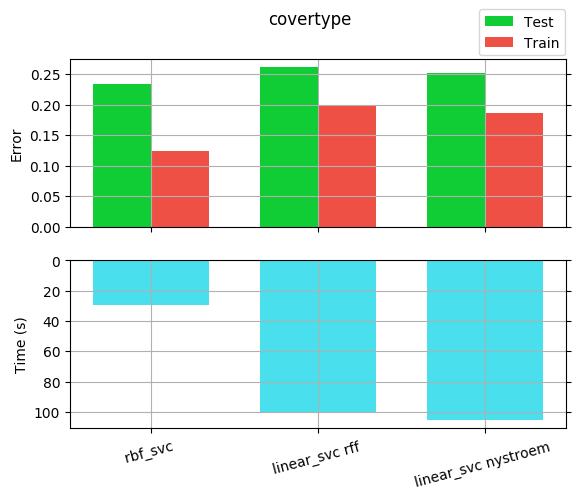
\includegraphics[width=\imgscale\linewidth]{Figures/1_1/covertype}
    \centering\captionsetup{width=.8\linewidth}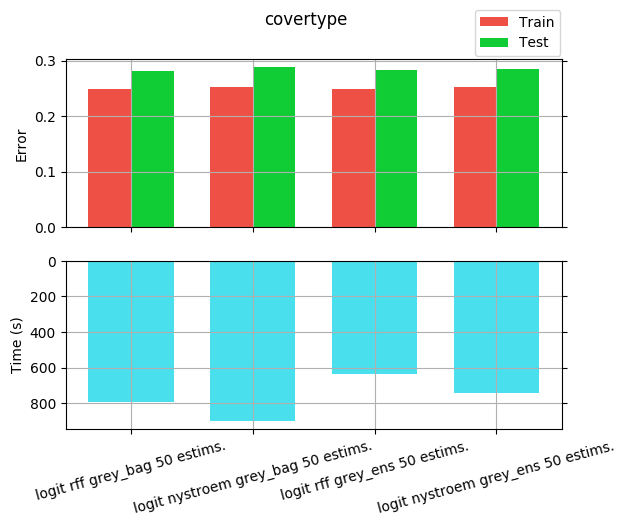
\includegraphics[width=\imgscale\linewidth]{Figures/\filePrefix/covertype}
    \caption{Exp. 1.1 with Covertype. SVM is outperformed}
    \label{fig:\undPrefix_covertype}
  \end{subfigure}%
  \begin{subfigure}[t]{0.5\linewidth}
    \centering\captionsetup{width=.8\linewidth}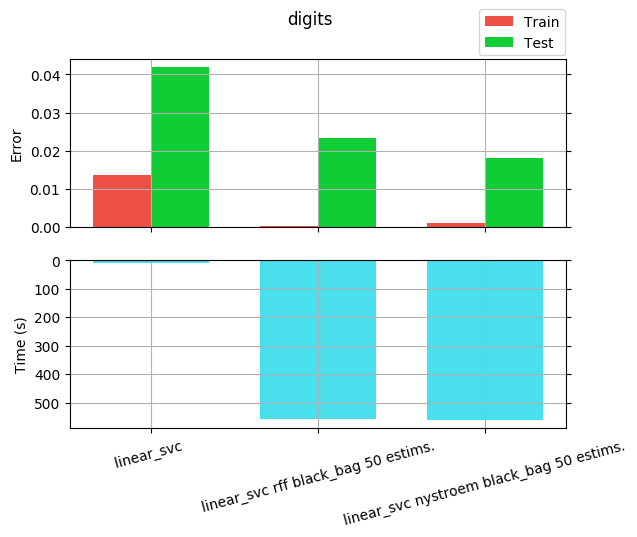
\includegraphics[width=\imgscale\linewidth]{Figures/\filePrefix/digits}
    \caption{Exp. 1.1 with Digits. SVM is outperformed}
    % \label{fig:1_1_digits}
    \label{fig:\undPrefix_digits}
  \end{subfigure}
\end{figure}


\begin{figure}[ht]
  \centering
  \begin{subfigure}[t]{0.5\linewidth}
    \centering\captionsetup{width=.8\linewidth}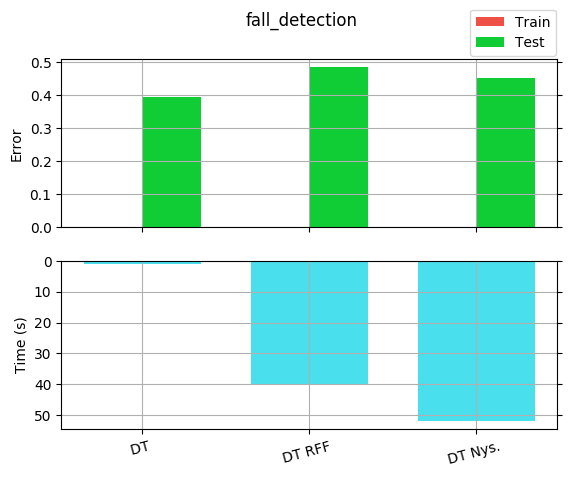
\includegraphics[width=\imgscale\linewidth]{Figures/\filePrefix/fall_detection}
    \caption{Exp. 1.1 with Fall Detection. RFF or \Nys\ can't outperform SVM}
    \label{fig:\undPrefix_fall_detection}
  \end{subfigure}%
  \begin{subfigure}[t]{0.5\linewidth}
    \centering\captionsetup{width=.8\linewidth}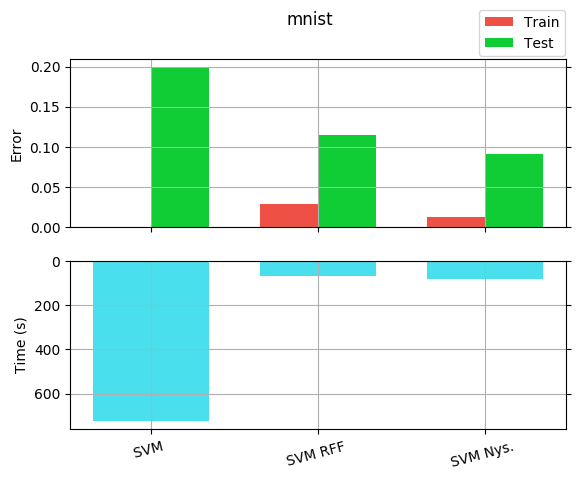
\includegraphics[width=\imgscale\linewidth]{Figures/\filePrefix/mnist}
    \caption{Exp. 1.1 with MNIST. SVM is outperformed}
    \label{fig:\undPrefix_mnist}
  \end{subfigure}
\end{figure}


\begin{figure}[ht]
  \centering
  \begin{subfigure}[t]{0.5\linewidth}
    \centering\captionsetup{width=.8\linewidth}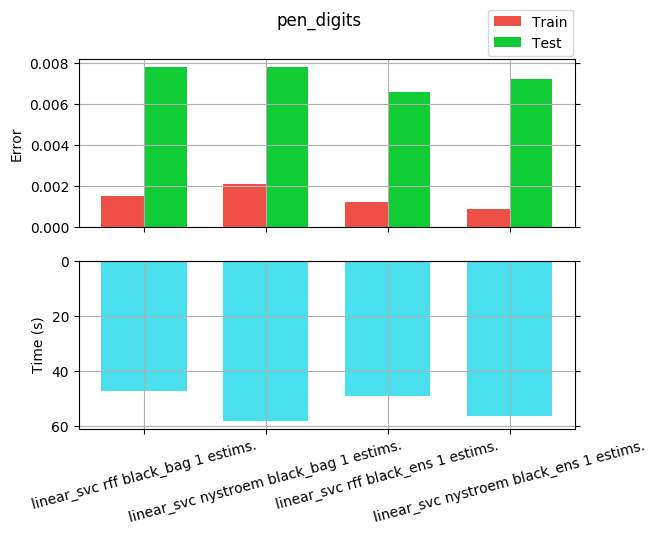
\includegraphics[width=\imgscale\linewidth]{Figures/\filePrefix/pen_digits}
    \caption{Exp. 1.1 with Pen Digits. SVM is outperformed}
    \label{fig:\undPrefix_pen_digits}
  \end{subfigure}%
  \begin{subfigure}[t]{0.5\linewidth}
    \centering\captionsetup{width=.8\linewidth}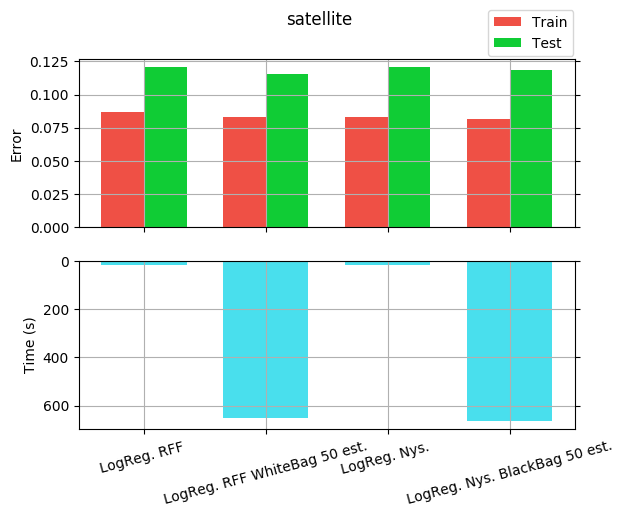
\includegraphics[width=\imgscale\linewidth]{Figures/\filePrefix/satellite}
    \caption{Exp. 1.1 with Satellite. SVM is outperformed}
    \label{fig:\undPrefix_satellite}
  \end{subfigure}
\end{figure}

\begin{figure}[ht]
  \centering
  \begin{subfigure}[t]{0.5\linewidth}
    \centering\captionsetup{width=.8\linewidth}
    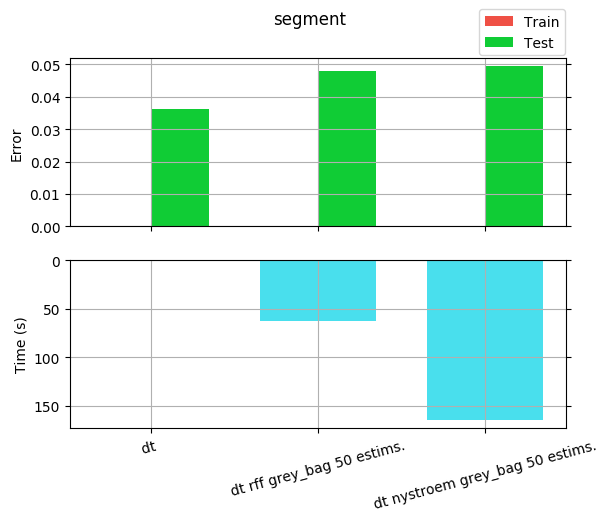
\includegraphics[width=\imgscale\linewidth]{Figures/\filePrefix/segment}
    \caption{Exp. 1.1 with Segment. SVM is outperformed}
    \label{fig:\undPrefix_segment}
  \end{subfigure}%
  \begin{subfigure}[t]{0.5\linewidth}
    \centering\captionsetup{width=.8\linewidth}
    \includegraphics[width=\imgscale\linewidth]{Figures/\filePrefix/vowel}
    \caption{Exp. 1.1 with Vowel. SVM is outperformed}
    \label{fig:\undPrefix_vowel}
  \end{subfigure}
\end{figure}

\begin{figure}[ht]
  \centering
  \begin{subfigure}[t]{0.5\linewidth}
    \centering\captionsetup{width=.8\linewidth}
    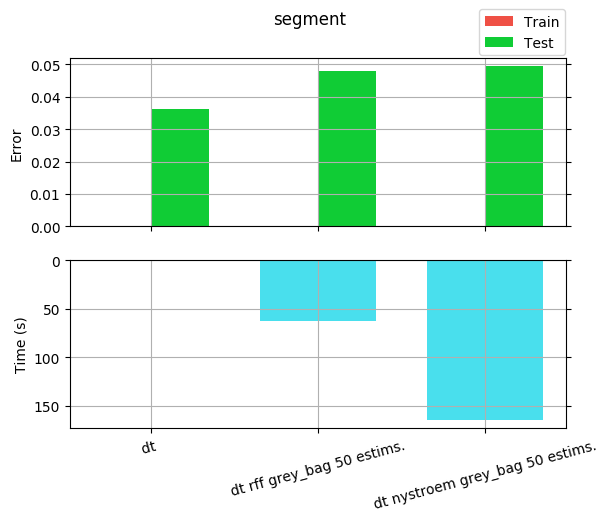
\includegraphics[width=\imgscale\linewidth]{Figures/\filePrefix/segment}
    \caption{Exp. 1.1 with Segment. SVM is outperformed}
    \label{fig:\undPrefix_segment}
  \end{subfigure}%
  \begin{subfigure}[t]{0.5\linewidth}
    \centering\captionsetup{width=.8\linewidth}
    \includegraphics[width=\imgscale\linewidth]{Figures/\filePrefix/vowel}
    \caption{Exp. 1.1 with Vowel. SVM is outperformed}
    \label{fig:\undPrefix_vowel}
  \end{subfigure}
\end{figure}


\let\major\undefined
\let\minor\undefined

\let\undPrefix\undefined
\let\dotPrefix\undefined
\let\scoPrefix\undefined

\let\filePrefix\undefined

% Appendix Template

\chapter{Results of experiment 1.1} % Main appendix title

\label{Appendix1-1} % Change X to a consecutive letter; for referencing this appendix elsewhere, use \ref{AppendixX}


\begin{figure}[ht]
  \centering
  \begin{subfigure}[b]{0.5\linewidth}
    \centering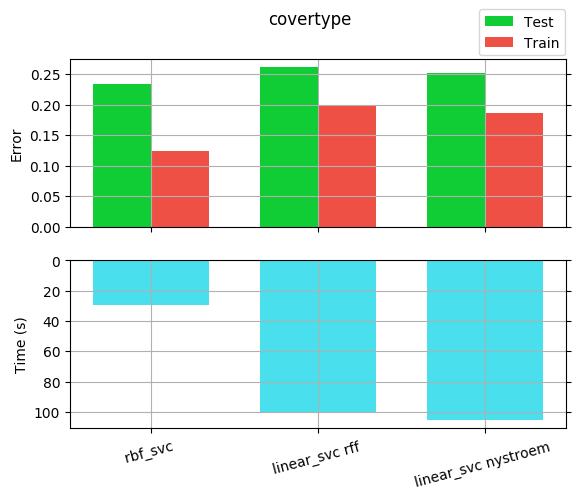
\includegraphics[width=\imgscale\linewidth]{Figures/1_1/covertype}
    \caption{prueba covertype}
    \label{fig:1_1_covertype}
  \end{subfigure}%
  \begin{subfigure}[b]{0.5\linewidth}
    \centering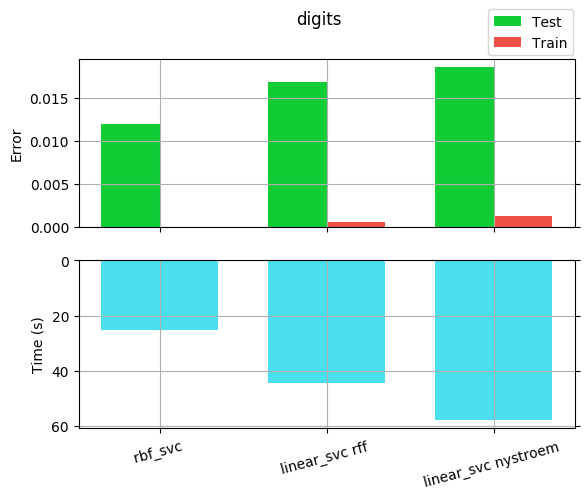
\includegraphics[width=\imgscale\linewidth]{Figures/1_1/digits}
    \caption{prueba digits}
    \label{fig:1_1_digits}
  \end{subfigure}
\end{figure}


\begin{figure}[ht]
  \centering
  \begin{subfigure}[b]{0.5\linewidth}
    \centering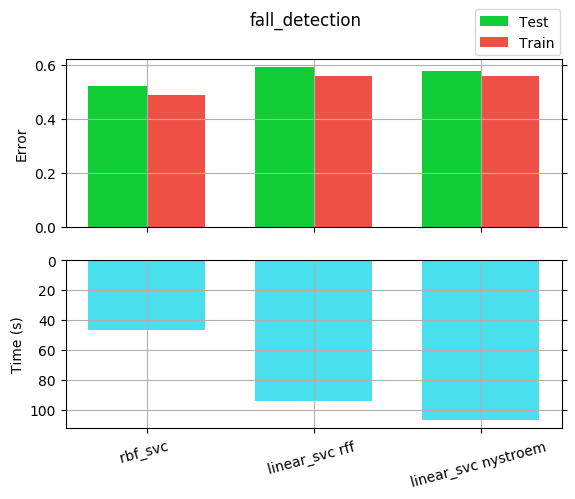
\includegraphics[width=\imgscale\linewidth]{Figures/1_1/fall_detection}
    \caption{prueba fall-detection}
    \label{fig:1_1_fall_detection}
  \end{subfigure}%
  \begin{subfigure}[b]{0.5\linewidth}
    \centering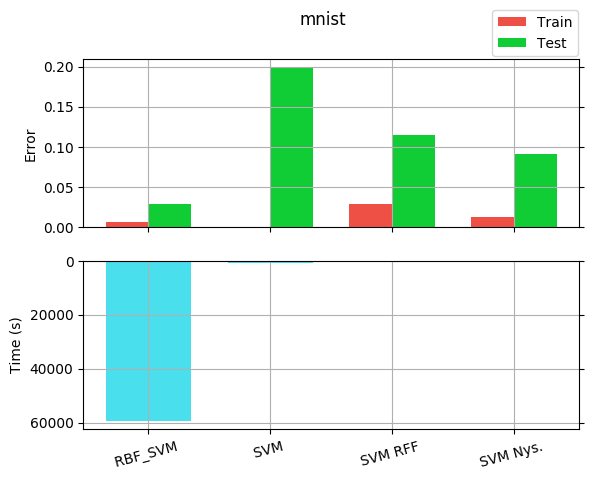
\includegraphics[width=\imgscale\linewidth]{Figures/1_1/mnist}
    \caption{prueba mnist}
    \label{fig:1_1_mnist}
  \end{subfigure}
\end{figure}


\begin{figure}[ht]
  \centering
  \begin{subfigure}[b]{0.5\linewidth}
    \centering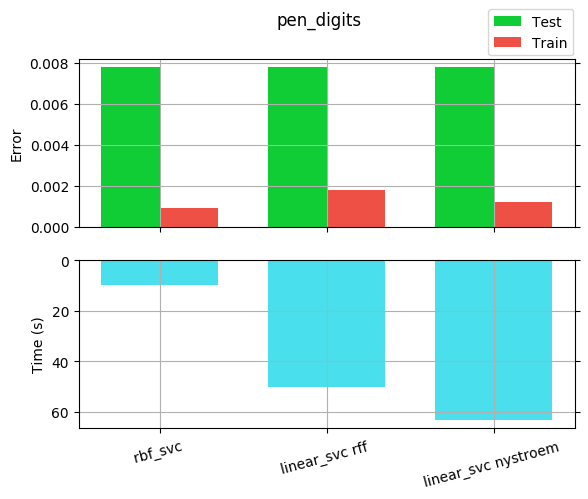
\includegraphics[width=\imgscale\linewidth]{Figures/1_1/pen_digits}
    \caption{prueba pen-digits}
    \label{fig:1_1_pen_digits}
  \end{subfigure}%
  \begin{subfigure}[b]{0.5\linewidth}
    \centering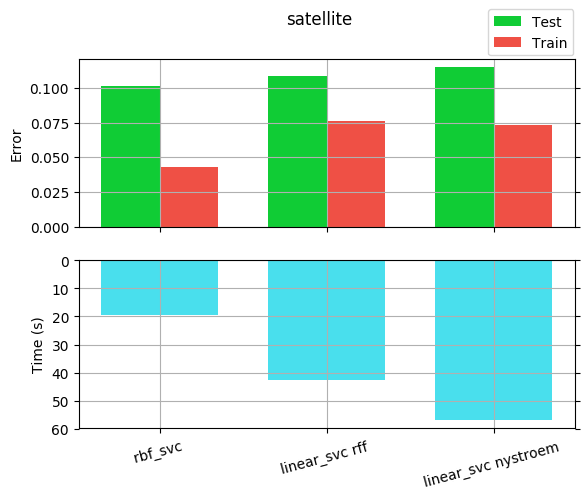
\includegraphics[width=\imgscale\linewidth]{Figures/1_1/satellite}
    \caption{prueba satellite}
    \label{fig:1_1_satellite}
  \end{subfigure}
\end{figure}

\begin{figure}[ht]
  \centering
  \begin{subfigure}[b]{0.5\linewidth}
    \centering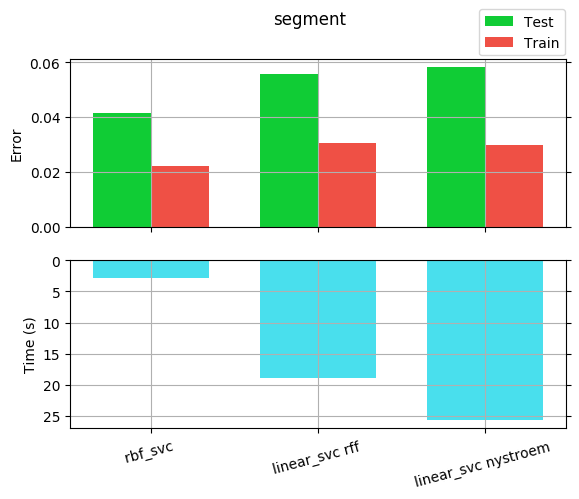
\includegraphics[width=\imgscale\linewidth]{Figures/1_1/segment}
    \caption{prueba segment}
    \label{fig:1_1_segment}
  \end{subfigure}%
  \begin{subfigure}[b]{0.5\linewidth}
    \centering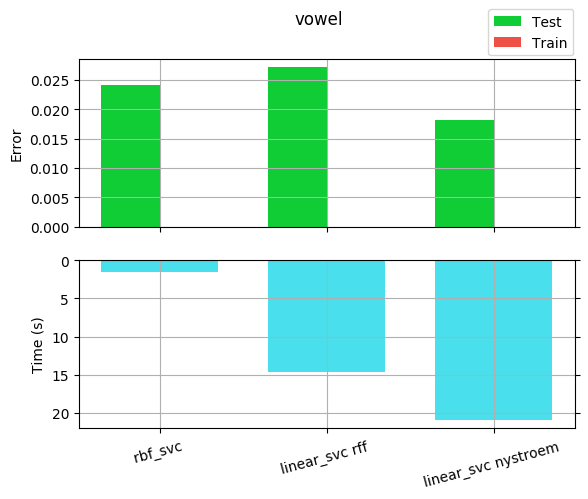
\includegraphics[width=\imgscale\linewidth]{Figures/1_1/vowel}
    \caption{prueba vowel}
    \label{fig:1_1_vowel}
  \end{subfigure}
\end{figure}

% Appendix Template

\chapter{Results of experiment 2.1} % Main appendix title

\label{Appendix2-1} % Change X to a consecutive letter; for referencing this appendix elsewhere, use \ref{AppendixX}

\begin{figure}[th]
\centering
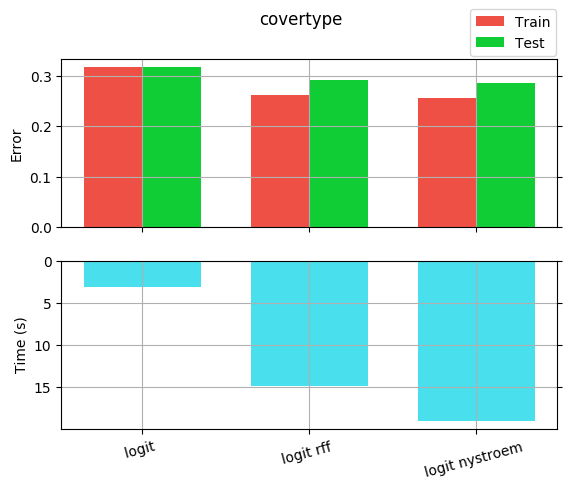
\includegraphics[scale=\imgscale]{Figures/2_1/covertype}
\decoRule
\caption[2.1 covertype]{Normal Logistic Regression and witdh RFF and \Nys}
\label{fig:2_1_covertype}
\end{figure}

\begin{figure}[th]
\centering
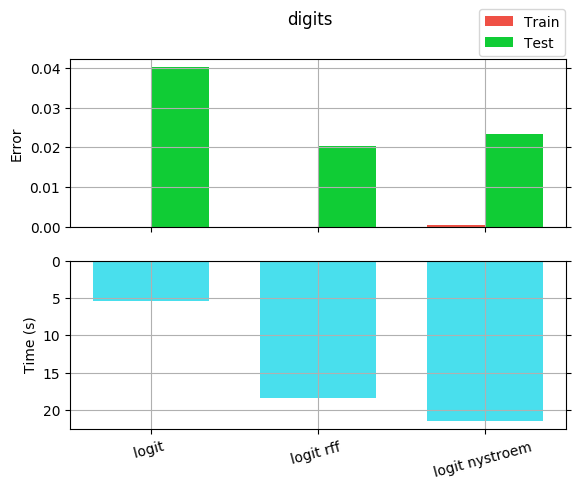
\includegraphics[scale=\imgscale]{Figures/2_1/digits}
\decoRule
\caption[2.1 digits]{Normal Logistic Regression and witdh RFF and \Nys}
\label{fig:2_1_digits}
\end{figure}

\begin{figure}[th]
\centering
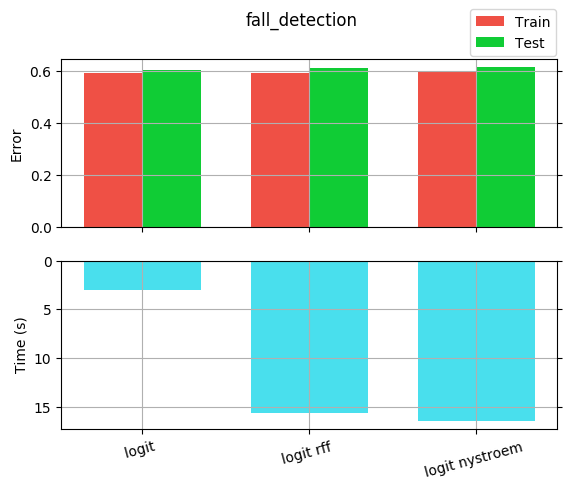
\includegraphics[scale=\imgscale]{Figures/2_1/fall_detection}
\decoRule
\caption[2.1 fall\tu detection]{Normal Logistic Regression and witdh RFF and \Nys}
\label{fig:2_1_fall_detection}
\end{figure}

\begin{figure}[th]
\centering
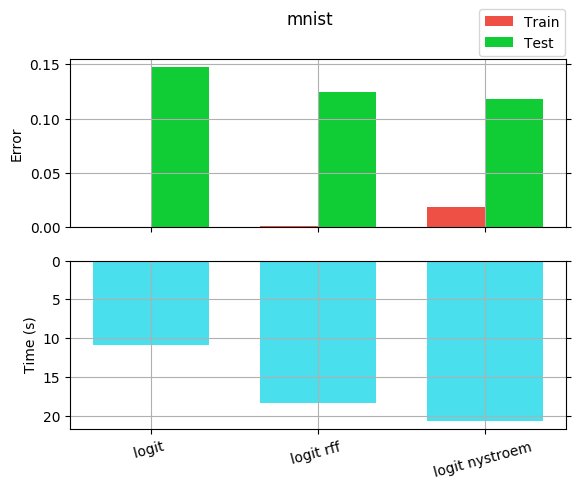
\includegraphics[scale=\imgscale]{Figures/2_1/mnist}
\decoRule
\caption[2.1 mnist]{Normal Logistic Regression and witdh RFF and \Nys}
\label{fig:2_1_mnist}
\end{figure}

\begin{figure}[th]
\centering
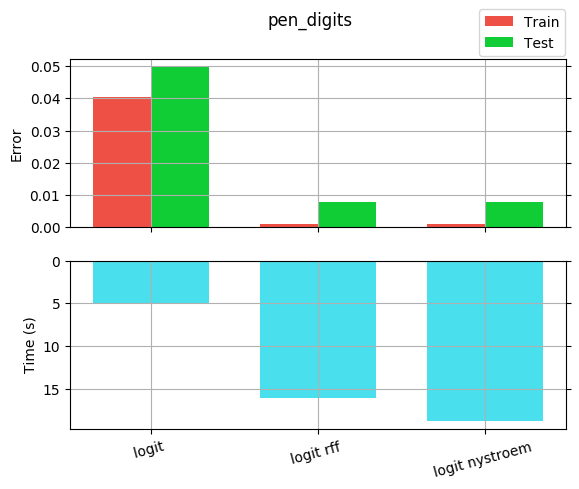
\includegraphics[scale=\imgscale]{Figures/2_1/pen_digits}
\decoRule
\caption[2.1 pen\tu digits]{Normal Logistic Regression and witdh RFF and \Nys}
\label{fig:2_1_pen_digits}
\end{figure}

\begin{figure}[th]
\centering
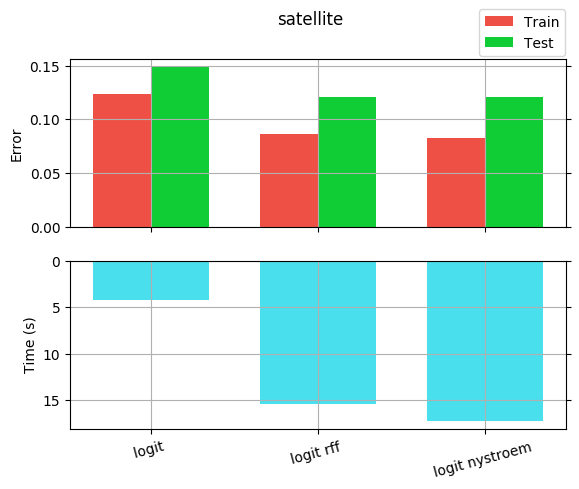
\includegraphics[scale=\imgscale]{Figures/2_1/satellite}
\decoRule
\caption[2.1 satellite]{Normal Logistic Regression and witdh RFF and \Nys}
\label{fig:2_1_satellite}
\end{figure}

\begin{figure}[th]
\centering
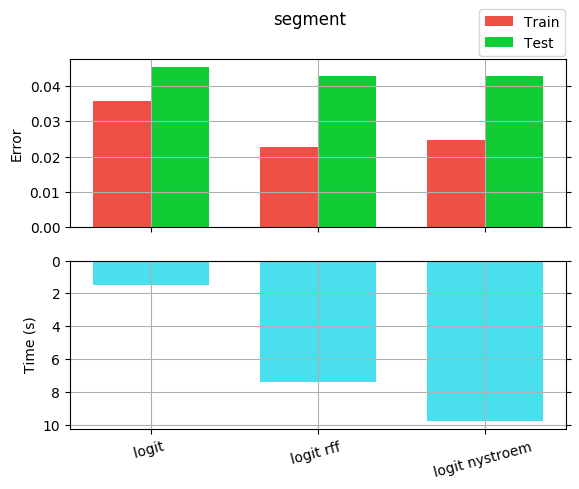
\includegraphics[scale=\imgscale]{Figures/2_1/segment}
\decoRule
\caption[2.1 segment]{Normal Logistic Regression and witdh RFF and \Nys}
\label{fig:2_1_segment}
\end{figure}

\begin{figure}[th]
\centering
\includegraphics[scale=\imgscale]{Figures/2_1/vowel}
\decoRule
\caption[2.1 vowel]{Normal Logistic Regression and witdh RFF and \Nys}
\label{fig:vowel}
\end{figure}

% Appendix Template

\chapter{Results of experiment 2.2} % Main appendix title

\label{Appendix2-2} % Change X to a consecutive letter; for referencing this appendix elsewhere, use \ref{AppendixX}

\begin{figure}[ht]
  \centering
  \begin{subfigure}[b]{0.5\linewidth}
    \centering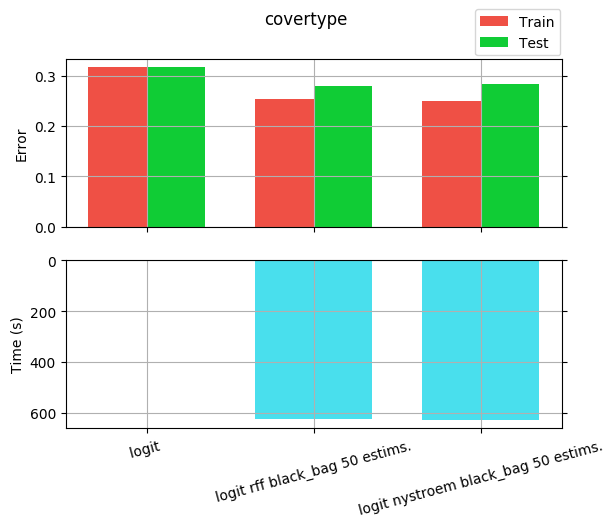
\includegraphics[width=\imgscale\linewidth]{Figures/2_2/covertype}
    \caption{prueba covertype}
    \label{fig:2_2_covertype}
  \end{subfigure}%
  \begin{subfigure}[b]{0.5\linewidth}
    \centering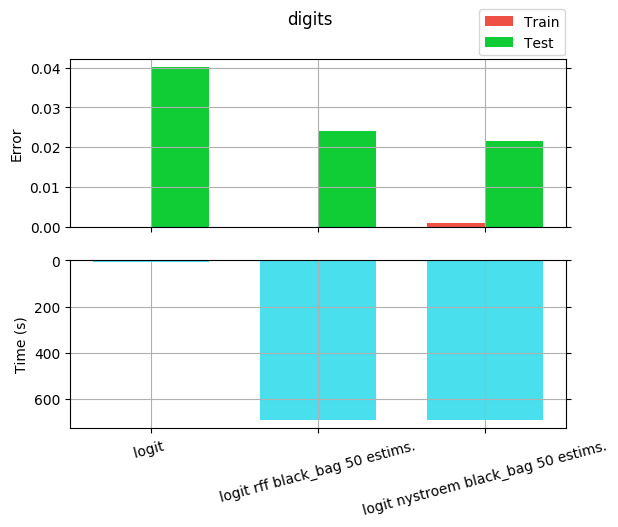
\includegraphics[width=\imgscale\linewidth]{Figures/2_2/digits}
    \caption{prueba digits}
    \label{fig:2_2_digits}
  \end{subfigure}
\end{figure}


\begin{figure}[ht]
  \centering
  \begin{subfigure}[b]{0.5\linewidth}
    \centering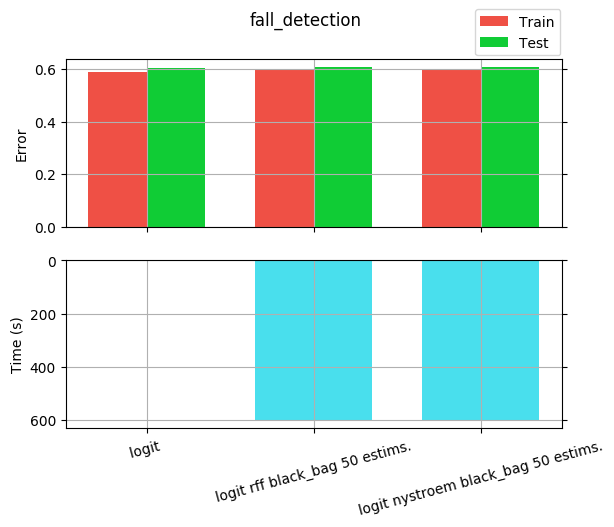
\includegraphics[width=\imgscale\linewidth]{Figures/2_2/fall_detection}
    \caption{prueba fall-detection}
    \label{fig:2_2_fall_detection}
  \end{subfigure}%
  \begin{subfigure}[b]{0.5\linewidth}
    \centering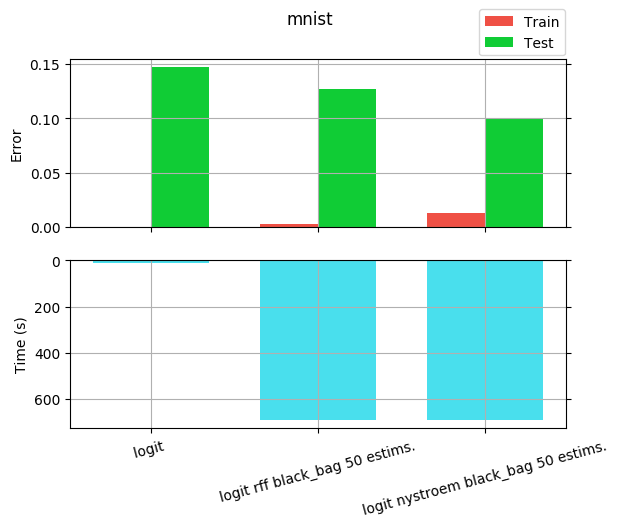
\includegraphics[width=\imgscale\linewidth]{Figures/2_2/mnist}
    \caption{prueba mnist}
    \label{fig:2_2_mnist}
  \end{subfigure}
\end{figure}


\begin{figure}[ht]
  \centering
  \begin{subfigure}[b]{0.5\linewidth}
    \centering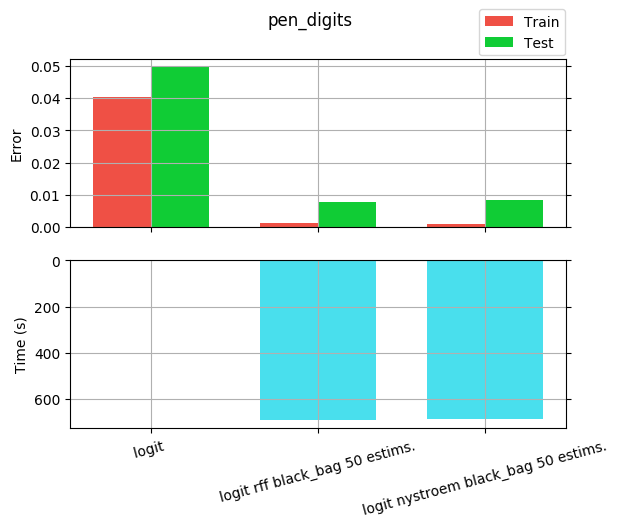
\includegraphics[width=\imgscale\linewidth]{Figures/2_2/pen_digits}
    \caption{prueba pen-digits}
    \label{fig:2_2_pen_digits}
  \end{subfigure}%
  \begin{subfigure}[b]{0.5\linewidth}
    \centering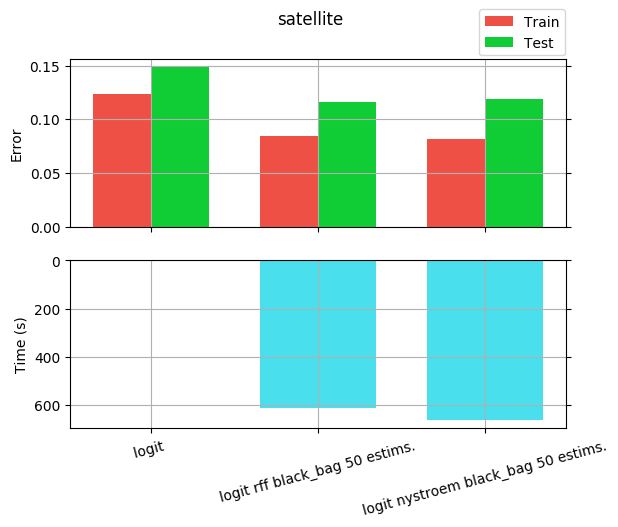
\includegraphics[width=\imgscale\linewidth]{Figures/2_2/satellite}
    \caption{prueba satellite}
    \label{fig:2_2_satellite}
  \end{subfigure}
\end{figure}

\begin{figure}[ht]
  \centering
  \begin{subfigure}[b]{0.5\linewidth}
    \centering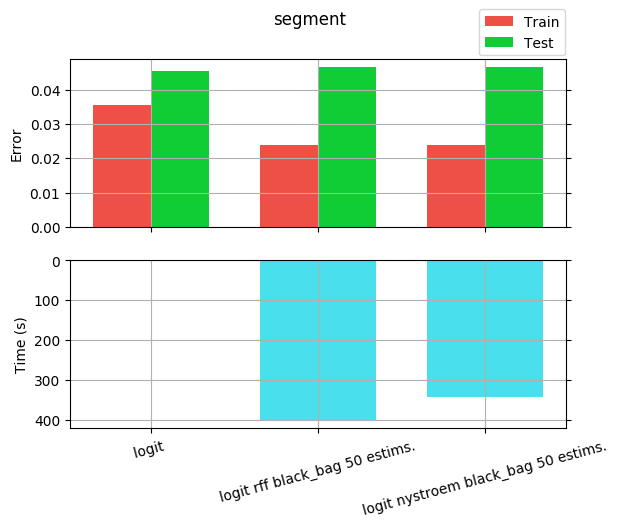
\includegraphics[width=\imgscale\linewidth]{Figures/2_2/segment}
    \caption{prueba segment}
    \label{fig:2_2_segment}
  \end{subfigure}%
  \begin{subfigure}[b]{0.5\linewidth}
    \centering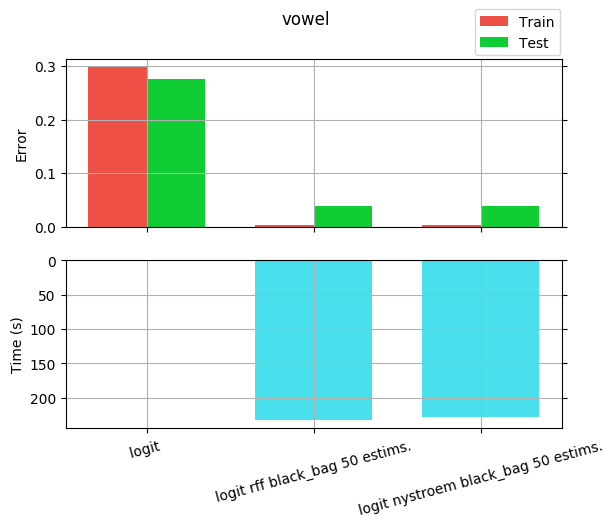
\includegraphics[width=\imgscale\linewidth]{Figures/2_2/vowel}
    \caption{prueba vowel}
    \label{fig:2_2_vowel}
  \end{subfigure}
\end{figure}

% Appendix Template

\newcommand{\major}{2}
\newcommand{\minor}{3}

\newcommand{\undPrefix}{\major_\minor}
\newcommand{\dotPrefix}{\major.\minor}
\newcommand{\scoPrefix}{\major-\minor}
\newcommand{\filePrefix}{\undPrefix}

\chapter{Results of experiment \dotPrefix} % Main appendix title


\label{Appendix\scoPrefix} % Change X to a consecutive letter; for referencing this appendix elsewhere, use \ref{AppendixX}
These experiments are discussed \hyperref[disc:h2]{here}

\begin{figure}[ht]
  \centering
  \begin{subfigure}[t]{0.5\linewidth}
    \centering\captionsetup{width=.8\linewidth}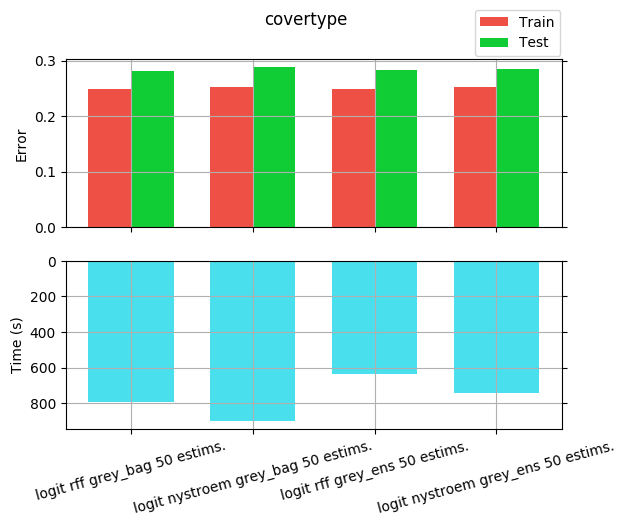
\includegraphics[width=\imgscale\linewidth]{Figures/\filePrefix/covertype}
    \caption{Exp 2.3 with Covertype. Error is decreased by 10\% approx.}
    \label{fig:\undPrefix_covertype}
  \end{subfigure}%
  \begin{subfigure}[t]{0.5\linewidth}
    \centering\captionsetup{width=.8\linewidth}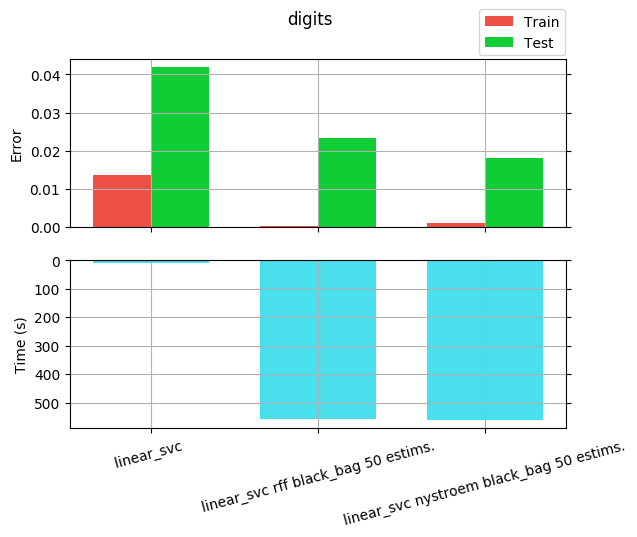
\includegraphics[width=\imgscale\linewidth]{Figures/\filePrefix/digits}
    \caption{Exp 2.3 with Digits. Error is decreased by 2\% approx.}
    \label{fig:\undPrefix_digits}
  \end{subfigure}
\end{figure}


\begin{figure}[ht]
  \centering
  \begin{subfigure}[t]{0.5\linewidth}
    \centering\captionsetup{width=.8\linewidth}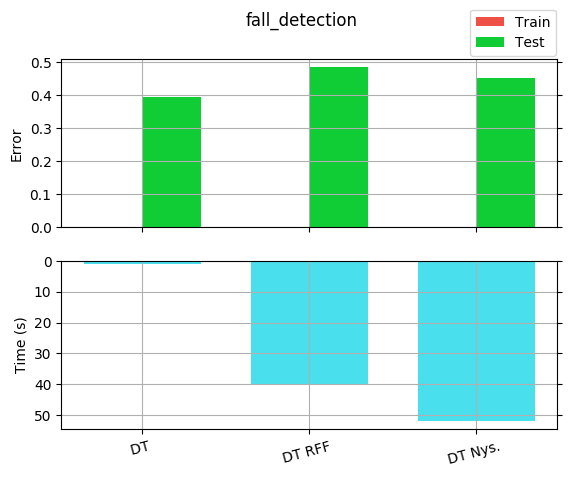
\includegraphics[width=\imgscale\linewidth]{Figures/\filePrefix/fall_detection}
    \caption{Exp 2.3 with Fall Detection. Error is not decreased.}
    \label{fig:\undPrefix_fall_detection}
  \end{subfigure}%
  \begin{subfigure}[t]{0.5\linewidth}
    \centering\captionsetup{width=.8\linewidth}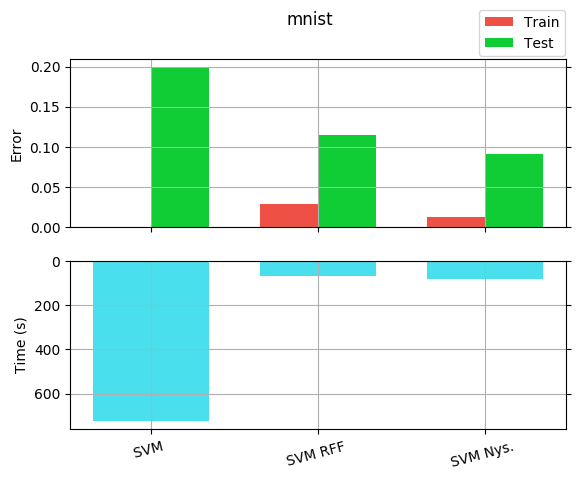
\includegraphics[width=\imgscale\linewidth]{Figures/\filePrefix/mnist}
    \caption{Exp 2.3 with MNIST. Error is decreased by 18\% approx.}
    \label{fig:\undPrefix_mnist}
  \end{subfigure}
\end{figure}


\begin{figure}[ht]
  \centering
  \begin{subfigure}[t]{0.5\linewidth}
    \centering\captionsetup{width=.8\linewidth}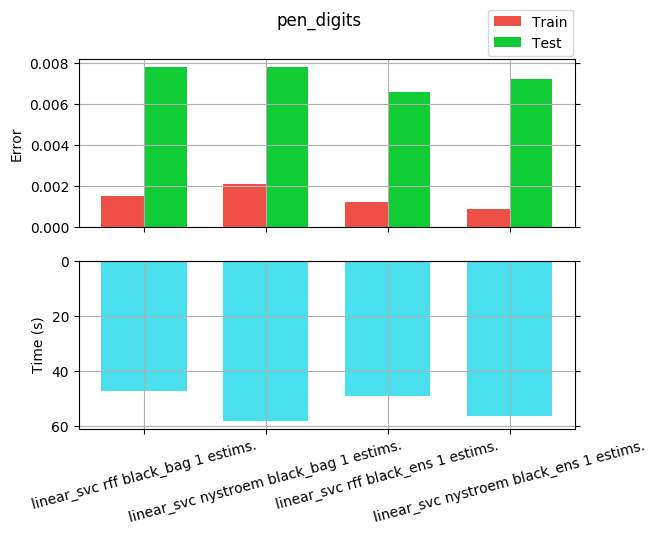
\includegraphics[width=\imgscale\linewidth]{Figures/\filePrefix/pen_digits}
    \caption{Exp 2.3 with Pen Digits. Error is decreased by 5\% approx.}
    \label{fig:\undPrefix_pen_digits}
  \end{subfigure}%
  \begin{subfigure}[t]{0.5\linewidth}
    \centering\captionsetup{width=.8\linewidth}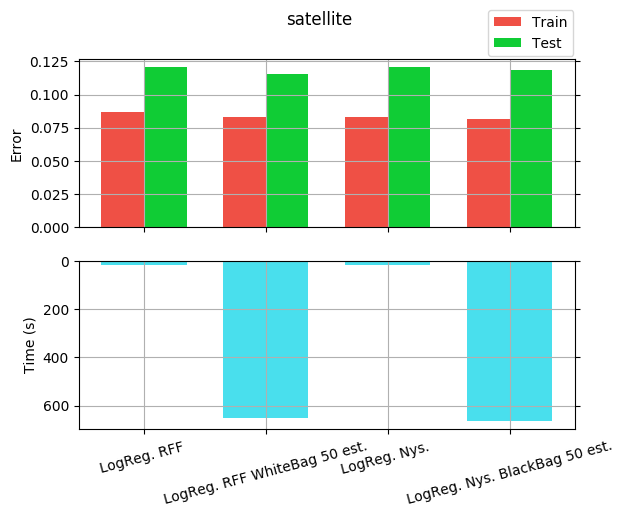
\includegraphics[width=\imgscale\linewidth]{Figures/\filePrefix/satellite}
    \caption{Exp 2.3 with Satellite. Error is decreased by 7\% approx.}
    \label{fig:\undPrefix_satellite}
  \end{subfigure}
\end{figure}

\begin{figure}[ht]
  \centering
  \begin{subfigure}[t]{0.5\linewidth}
    \centering\captionsetup{width=.8\linewidth}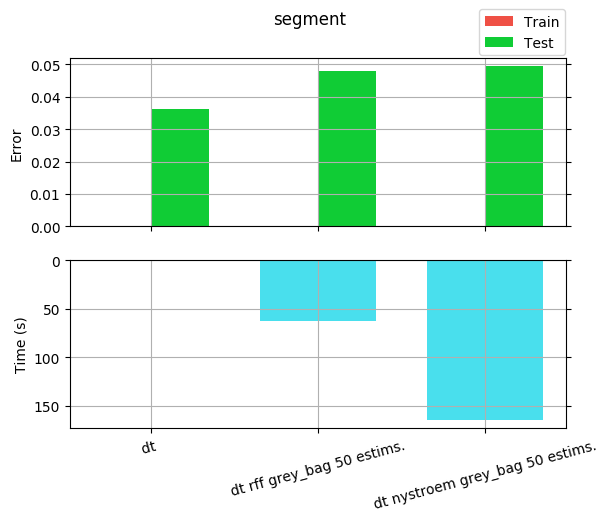
\includegraphics[width=\imgscale\linewidth]{Figures/\filePrefix/segment}
    \caption{Exp 2.3 with Segment. Error is decreased by 2\% approx.}
    \label{fig:\undPrefix_segment}
  \end{subfigure}%
  \begin{subfigure}[t]{0.5\linewidth}
    \centering\captionsetup{width=.8\linewidth}\includegraphics[width=\imgscale\linewidth]{Figures/\filePrefix/vowel}
    \caption{Exp 2.3 with Vowel. Error is decreased by 35\% approx.}
    \label{fig:\undPrefix_vowel}
  \end{subfigure}
\end{figure}


\let\major\undefined
\let\minor\undefined

\let\undPrefix\undefined
\let\dotPrefix\undefined
\let\scoPrefix\undefined

\let\filePrefix\undefined

% Appendix Template

\chapter{Results of experiment 2.4} % Main appendix title

\label{Appendix2-4} % Change X to a consecutive letter; for referencing this appendix elsewhere, use \ref{AppendixX}

\begin{figure}[th]
\centering
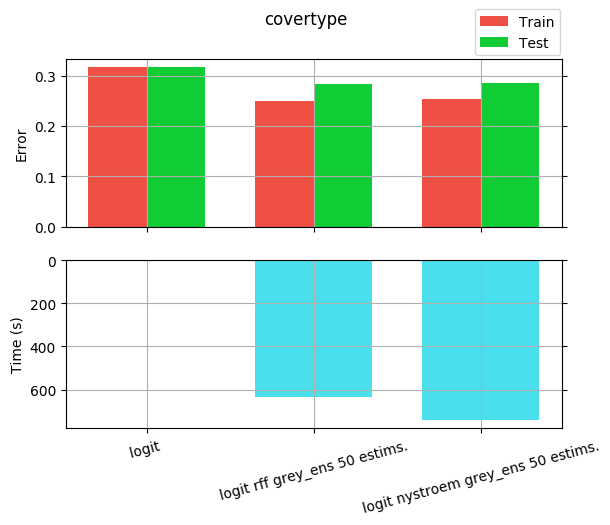
\includegraphics[scale=\imgscale]{Figures/2_4/covertype}
\decoRule
\caption[2.4 covertype]{Logistic Regression with Grey Ensemble model}
\label{fig:2_4_covertype}
\end{figure}

\begin{figure}[th]
\centering
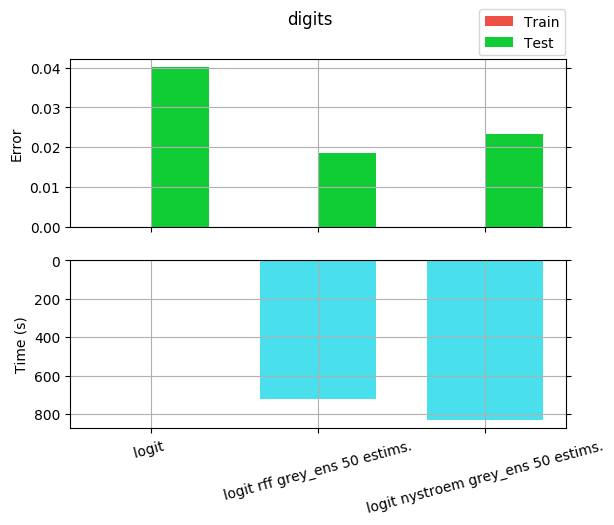
\includegraphics[scale=\imgscale]{Figures/2_4/digits}
\decoRule
\caption[2.4 digits]{Logistic Regression with Grey Ensemble model}
\label{fig:2_4_digits}
\end{figure}

\begin{figure}[th]
\centering
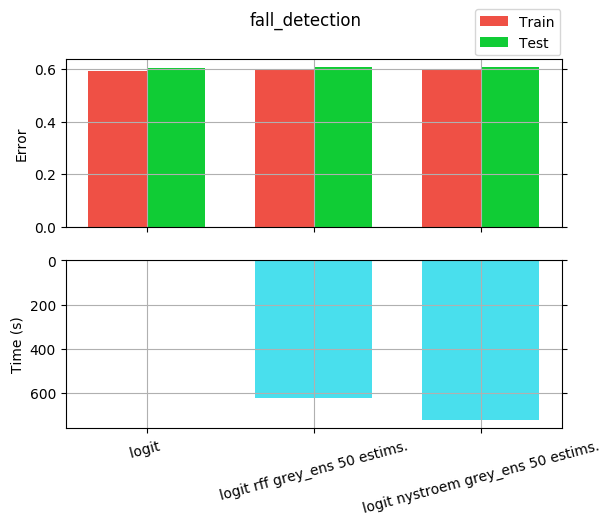
\includegraphics[scale=\imgscale]{Figures/2_4/fall_detection}
\decoRule
\caption[2.4 fall\tu detection]{Logistic Regression with Grey Ensemble model}
\label{fig:2_4_fall_detection}
\end{figure}

\begin{figure}[th]
\centering
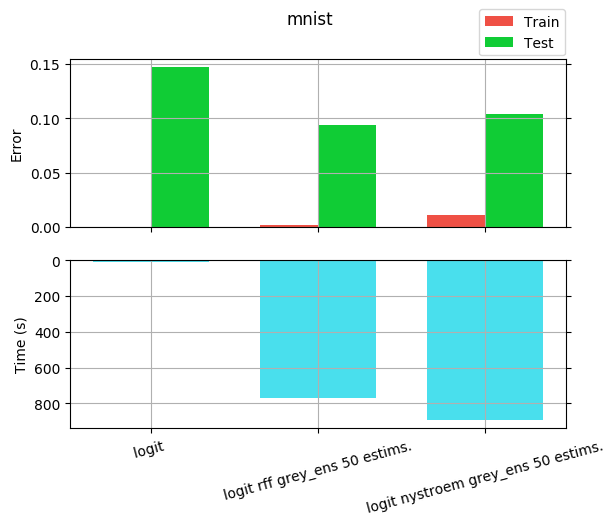
\includegraphics[scale=\imgscale]{Figures/2_4/mnist}
\decoRule
\caption[2.4 mnist]{Logistic Regression with Grey Ensemble model}
\label{fig:2_4_mnist}
\end{figure}

\begin{figure}[th]
\centering
\includegraphics[scale=\imgscale]{Figures/2_4/pen_digits}
\decoRule
\caption[2.4 pen\tu digits]{Logistic Regression with Grey Ensemble model}
\label{fig:2_4_pen_digits}
\end{figure}

\begin{figure}[th]
\centering
\includegraphics[scale=\imgscale]{Figures/2_4/satellite}
\decoRule
\caption[2.4 satellite]{Logistic Regression with Grey Ensemble model}
\label{fig:2_4_satellite}
\end{figure}

\begin{figure}[th]
\centering
\includegraphics[scale=\imgscale]{Figures/2_4/segment}
\decoRule
\caption[2.4 segment]{Logistic Regression with Grey Ensemble model}
\label{fig:2_4_segment}
\end{figure}

\begin{figure}[th]
\centering
\includegraphics[scale=\imgscale]{Figures/2_4/vowel}
\decoRule
\caption[2.4 vowel]{Logistic Regression with Grey Ensemble model}
\label{fig:vowel}
\end{figure}


% Appendix Template

\newcommand{\major}{3}
\newcommand{\minor}{1}

\newcommand{\undPrefix}{\major_\minor}
\newcommand{\dotPrefix}{\major.\minor}
\newcommand{\scoPrefix}{\major-\minor}
\newcommand{\filePrefix}{\undPrefix}

% \chapter{Results of experiment 1.1} % Main appendix title
\chapter{Results of experiment \dotPrefix} % Main appendix title

% \label{Appendix1-1} % Change X to a consecutive letter; for referencing this appendix elsewhere, use \ref{AppendixX}

\label{Appendix\scoPrefix} % Change X to a consecutive letter; for referencing this appendix elsewhere, use \ref{AppendixX}

These experiments are discussed \hyperref[disc:h3]{here}
\begin{figure}[ht]
  \centering
  \begin{subfigure}[t]{0.5\linewidth}
    % \centering\captionsetup{width=.8\linewidth}\includegraphics[width=\imgscale\linewidth]{Figures/1_1/covertype}
    \centering\captionsetup{width=.8\linewidth}\includegraphics[width=\imgscale\linewidth]{Figures/\filePrefix/covertype}
    \caption{Exp. 3.1 with Covertype. White Box Models with Logistic Regression. There is not much difference between Box Models}
    \label{fig:\undPrefix_covertype}
  \end{subfigure}%
  \begin{subfigure}[t]{0.5\linewidth}
    \centering\captionsetup{width=.8\linewidth}\includegraphics[width=\imgscale\linewidth]{Figures/\filePrefix/digits}
    \caption{Exp. 3.1 with Digits. White Box Models with Logistic Regression. There is not much difference between Box Models}
    % \label{fig:1_1_digits}
    \label{fig:\undPrefix_digits}
  \end{subfigure}
\end{figure}


\begin{figure}[ht]
  \centering
  \begin{subfigure}[t]{0.5\linewidth}
    \centering\captionsetup{width=.8\linewidth}\includegraphics[width=\imgscale\linewidth]{Figures/\filePrefix/fall_detection}
    \caption{Exp. 3.1 with Fall Detection. White Box Models with Logistic Regression. There is not much difference between Box Models}
    \label{fig:\undPrefix_fall_detection}
  \end{subfigure}%
  \begin{subfigure}[t]{0.5\linewidth}
    \centering\captionsetup{width=.8\linewidth}\includegraphics[width=\imgscale\linewidth]{Figures/\filePrefix/mnist}
    \caption{Exp. 3.1 with MNIST. White Box Models with Logistic Regression. There is not much difference between Box Models}
    \label{fig:\undPrefix_mnist}
  \end{subfigure}
\end{figure}


\begin{figure}[ht]
  \centering
  \begin{subfigure}[t]{0.5\linewidth}
    \centering\captionsetup{width=.8\linewidth}\includegraphics[width=\imgscale\linewidth]{Figures/\filePrefix/pen_digits}
    \caption{Exp. 3.1 with Pen Digits. White Box Models with Logistic Regression. There is not much difference between Box Models}
    \label{fig:\undPrefix_pen_digits}
  \end{subfigure}%
  \begin{subfigure}[t]{0.5\linewidth}
    \centering\captionsetup{width=.8\linewidth}\includegraphics[width=\imgscale\linewidth]{Figures/\filePrefix/satellite}
    \caption{Exp. 3.1 with Satelite. White Box Models with Logistic Regression. There is not much difference between Box Models}
    \label{fig:\undPrefix_satellite}
  \end{subfigure}
\end{figure}

\begin{figure}[ht]
  \centering
  \begin{subfigure}[t]{0.5\linewidth}
    \centering\captionsetup{width=.8\linewidth}\includegraphics[width=\imgscale\linewidth]{Figures/\filePrefix/segment}
    \caption{Exp. 3.1 with Segment. White Box Models with Logistic Regression. There is not much difference between Box Models}
    \label{fig:\undPrefix_segment}
  \end{subfigure}%
  \begin{subfigure}[t]{0.5\linewidth}
    \centering\captionsetup{width=.8\linewidth}\includegraphics[width=\imgscale\linewidth]{Figures/\filePrefix/vowel}
    \caption{Exp. 3.1 with Vowel. White Box Models with Logistic Regression. There is not much difference between Box Models}
    \label{fig:\undPrefix_vowel}
  \end{subfigure}
\end{figure}


\let\major\undefined
\let\minor\undefined

\let\undPrefix\undefined
\let\dotPrefix\undefined
\let\scoPrefix\undefined

\let\filePrefix\undefined

% Appendix Template

\newcommand{\major}{3}
\newcommand{\minor}{2}

\newcommand{\undPrefix}{\major_\minor}
\newcommand{\dotPrefix}{\major.\minor}
\newcommand{\scoPrefix}{\major-\minor}
\newcommand{\filePrefix}{\undPrefix}

% \chapter{Results of experiment 1.1} % Main appendix title
\chapter{Results of experiment \dotPrefix} % Main appendix title

% \label{Appendix1-1} % Change X to a consecutive letter; for referencing this appendix elsewhere, use \ref{AppendixX}

\label{Appendix\scoPrefix} % Change X to a consecutive letter; for referencing this appendix elsewhere, use \ref{AppendixX}

These experiments are discussed \hyperref[disc:h3]{here}
\begin{figure}[ht]
  \centering
  \begin{subfigure}[t]{0.5\linewidth}
    % \centering\captionsetup{width=.8\linewidth}\includegraphics[width=\imgscale\linewidth]{Figures/1_1/covertype}
    \centering\captionsetup{width=.8\linewidth}\includegraphics[width=\imgscale\linewidth]{Figures/\filePrefix/covertype}
    \caption{Exp. 3.2 with Covertype. Black Box Models with Logistic Regression. There is not much difference between Box Models}
    \label{fig:\undPrefix_covertype}
  \end{subfigure}%
  \begin{subfigure}[t]{0.5\linewidth}
    \centering\captionsetup{width=.8\linewidth}\includegraphics[width=\imgscale\linewidth]{Figures/\filePrefix/digits}
    \caption{Exp. 3.2 with Digits. Black Box Models with Logistic Regression. There is not much difference between Box Models}
    % \label{fig:1_1_digits}
    \label{fig:\undPrefix_digits}
  \end{subfigure}
\end{figure}


\begin{figure}[ht]
  \centering
  \begin{subfigure}[t]{0.5\linewidth}
    \centering\captionsetup{width=.8\linewidth}\includegraphics[width=\imgscale\linewidth]{Figures/\filePrefix/fall_detection}
    \caption{Exp. 3.2 with Fall Detection. Black Box Models with Logistic Regression. There is not much difference between Box Models}
    \label{fig:\undPrefix_fall_detection}
  \end{subfigure}%
  \begin{subfigure}[t]{0.5\linewidth}
    \centering\captionsetup{width=.8\linewidth}\includegraphics[width=\imgscale\linewidth]{Figures/\filePrefix/mnist}
    \caption{Exp. 3.2 with MNIST. Black Box Models with Logistic Regression. There is not much difference between Box Models}
    \label{fig:\undPrefix_mnist}
  \end{subfigure}
\end{figure}


\begin{figure}[ht]
  \centering
  \begin{subfigure}[t]{0.5\linewidth}
    \centering\captionsetup{width=.8\linewidth}\includegraphics[width=\imgscale\linewidth]{Figures/\filePrefix/pen_digits}
    \caption{Exp. 3.2 with Pen Digits. Black Box Models with Logistic Regression. There is not much difference between Box Models}
    \label{fig:\undPrefix_pen_digits}
  \end{subfigure}%
  \begin{subfigure}[t]{0.5\linewidth}
    \centering\captionsetup{width=.8\linewidth}\includegraphics[width=\imgscale\linewidth]{Figures/\filePrefix/satellite}
    \caption{Exp. 3.2 with Satellite. Black Box Models with Logistic Regression. There is not much difference between Box Models}
    \label{fig:\undPrefix_satellite}
  \end{subfigure}
\end{figure}

\begin{figure}[ht]
  \centering
  \begin{subfigure}[t]{0.5\linewidth}
    \centering\captionsetup{width=.8\linewidth}\includegraphics[width=\imgscale\linewidth]{Figures/\filePrefix/segment}
    \caption{Exp. 3.2 with Segment. Black Box Models with Logistic Regression. There is not much difference between Box Models}
    \label{fig:\undPrefix_segment}
  \end{subfigure}%
  \begin{subfigure}[t]{0.5\linewidth}
    \centering\captionsetup{width=.8\linewidth}\includegraphics[width=\imgscale\linewidth]{Figures/\filePrefix/vowel}
    \caption{Exp. 3.2 with Vowel. Black Box Models with Logistic Regression.
    Ensemble with decreases error by 2\%}
    \label{fig:\undPrefix_vowel}
  \end{subfigure}
\end{figure}


\begin{figure}[ht]
  \centering
  \begin{subfigure}[t]{0.5\linewidth}
    \centering\captionsetup{width=.8\linewidth}\includegraphics[width=\imgscale\linewidth]{Figures/\filePrefix/fashion_mnist}
    \caption{Exp. 3.2 with Fashion MNIST. Black Box Models with Logistic Regression. There is not much difference between Box Models}
    \label{fig:\undPrefix_segment}
  \end{subfigure}%
\end{figure}


\let\major\undefined
\let\minor\undefined

\let\undPrefix\undefined
\let\dotPrefix\undefined
\let\scoPrefix\undefined

\let\filePrefix\undefined

% Appendix Template

\newcommand{\major}{3}
\newcommand{\minor}{3}

\newcommand{\undPrefix}{\major_\minor}
\newcommand{\dotPrefix}{\major.\minor}
\newcommand{\scoPrefix}{\major-\minor}
\newcommand{\filePrefix}{\undPrefix}

% \chapter{Results of experiment 1.1} % Main appendix title
\chapter{Results of experiment \dotPrefix} % Main appendix title

% \label{Appendix1-1} % Change X to a consecutive letter; for referencing this appendix elsewhere, use \ref{AppendixX}

\label{Appendix\scoPrefix} % Change X to a consecutive letter; for referencing this appendix elsewhere, use \ref{AppendixX}

These experiments are discussed \hyperref[disc:h3]{here}
\begin{figure}[ht]
  \centering
  \begin{subfigure}[t]{0.5\linewidth}
    % \centering\captionsetup{width=.8\linewidth}\includegraphics[width=\imgscale\linewidth]{Figures/1_1/covertype}
    \centering\captionsetup{width=.8\linewidth}\includegraphics[width=\imgscale\linewidth]{Figures/\filePrefix/covertype}
    \caption{Exp. 3.3 with Covertype. White Box Models with Support Vector Machine. There is not much difference between Box Models}
    \label{fig:\undPrefix_covertype}
  \end{subfigure}%
  \begin{subfigure}[t]{0.5\linewidth}
    \centering\captionsetup{width=.8\linewidth}\includegraphics[width=\imgscale\linewidth]{Figures/\filePrefix/digits}
    \caption{Exp. 3.3 with Digits. White Box Models with Support Vector Machine. There is not much difference between Box Models}
    % \label{fig:1_1_digits}
    \label{fig:\undPrefix_digits}
  \end{subfigure}
\end{figure}


\begin{figure}[ht]
  \centering
  \begin{subfigure}[t]{0.5\linewidth}
    \centering\captionsetup{width=.8\linewidth}\includegraphics[width=\imgscale\linewidth]{Figures/\filePrefix/fall_detection}
    \caption{Exp. 3.3 with Fall Detection. White Box Models with Support Vector Machine. There is not much difference between Box Models}
    \label{fig:\undPrefix_fall_detection}
  \end{subfigure}%
  \begin{subfigure}[t]{0.5\linewidth}
    \centering\captionsetup{width=.8\linewidth}\includegraphics[width=\imgscale\linewidth]{Figures/\filePrefix/mnist}
    \caption{Exp. 3.3 with MNIST. White Box Models with Support Vector Machine. There is not much difference between Box Models}
    \label{fig:\undPrefix_mnist}
  \end{subfigure}
\end{figure}


\begin{figure}[ht]
  \centering
  \begin{subfigure}[t]{0.5\linewidth}
    \centering\captionsetup{width=.8\linewidth}\includegraphics[width=\imgscale\linewidth]{Figures/\filePrefix/pen_digits}
    \caption{Exp. 3.3 with Pen Digits. White Box Models with Support Vector Machine. There is not much difference between Box Models}
    \label{fig:\undPrefix_pen_digits}
  \end{subfigure}%
  \begin{subfigure}[t]{0.5\linewidth}
    \centering\captionsetup{width=.8\linewidth}\includegraphics[width=\imgscale\linewidth]{Figures/\filePrefix/satellite}
    \caption{Exp. 3.3 with Satellite. White Box Models with Support Vector Machine. There is not much difference between Box Models}
    \label{fig:\undPrefix_satellite}
  \end{subfigure}
\end{figure}

\begin{figure}[ht]
  \centering
  \begin{subfigure}[t]{0.5\linewidth}
    \centering\captionsetup{width=.8\linewidth}\includegraphics[width=\imgscale\linewidth]{Figures/\filePrefix/segment}
    \caption{Exp. 3.3 with Segment. White Box Models with Support Vector Machine. There is not much difference between Box Models}
    \label{fig:\undPrefix_segment}
  \end{subfigure}%
  \begin{subfigure}[t]{0.5\linewidth}
    \centering\captionsetup{width=.8\linewidth}\includegraphics[width=\imgscale\linewidth]{Figures/\filePrefix/vowel}
    \caption{Exp. 3.3 with Vowel. White Box Models with Support Vector Machine. There is not much difference between Box Models}
    \label{fig:\undPrefix_vowel}
  \end{subfigure}
\end{figure}


\begin{figure}[ht]
  \centering
  \begin{subfigure}[t]{0.5\linewidth}
    \centering\captionsetup{width=.8\linewidth}\includegraphics[width=\imgscale\linewidth]{Figures/\filePrefix/fashion_mnist}
    \caption{Exp. 3.3 with Fashion MNIST. White Box Models with Support Vector Machine. There is not much difference between Box Models}
    \label{fig:\undPrefix_segment}
  \end{subfigure}%
\end{figure}


\let\major\undefined
\let\minor\undefined

\let\undPrefix\undefined
\let\dotPrefix\undefined
\let\scoPrefix\undefined

\let\filePrefix\undefined

% Appendix Template

\newcommand{\major}{3}
\newcommand{\minor}{4}

\newcommand{\undPrefix}{\major_\minor}
\newcommand{\dotPrefix}{\major.\minor}
\newcommand{\scoPrefix}{\major-\minor}
\newcommand{\filePrefix}{\undPrefix}

% \chapter{Results of experiment 1.1} % Main appendix title
\chapter{Results of experiment \dotPrefix} % Main appendix title

% \label{Appendix1-1} % Change X to a consecutive letter; for referencing this appendix elsewhere, use \ref{AppendixX}

\label{Appendix\scoPrefix} % Change X to a consecutive letter; for referencing this appendix elsewhere, use \ref{AppendixX}


\begin{figure}[ht]
  \centering
  \begin{subfigure}[b]{0.5\linewidth}
    % \centering\includegraphics[width=\imgscale\linewidth]{Figures/1_1/covertype}
    \centering\includegraphics[width=\imgscale\linewidth]{Figures/\filePrefix/covertype}
    \caption{prueba covertype}
    \label{fig:\undPrefix_covertype}
  \end{subfigure}%
  \begin{subfigure}[b]{0.5\linewidth}
    \centering\includegraphics[width=\imgscale\linewidth]{Figures/\filePrefix/digits}
    \caption{prueba digits}
    % \label{fig:1_1_digits}
    \label{fig:\undPrefix_digits}
  \end{subfigure}
\end{figure}


\begin{figure}[ht]
  \centering
  \begin{subfigure}[b]{0.5\linewidth}
    \centering\includegraphics[width=\imgscale\linewidth]{Figures/\filePrefix/fall_detection}
    \caption{prueba fall-detection}
    \label{fig:\undPrefix_fall_detection}
  \end{subfigure}%
  \begin{subfigure}[b]{0.5\linewidth}
    \centering\includegraphics[width=\imgscale\linewidth]{Figures/\filePrefix/mnist}
    \caption{prueba mnist}
    \label{fig:\undPrefix_mnist}
  \end{subfigure}
\end{figure}


\begin{figure}[ht]
  \centering
  \begin{subfigure}[b]{0.5\linewidth}
    \centering\includegraphics[width=\imgscale\linewidth]{Figures/\filePrefix/pen_digits}
    \caption{prueba pen-digits}
    \label{fig:\undPrefix_pen_digits}
  \end{subfigure}%
  \begin{subfigure}[b]{0.5\linewidth}
    \centering\includegraphics[width=\imgscale\linewidth]{Figures/\filePrefix/satellite}
    \caption{prueba satellite}
    \label{fig:\undPrefix_satellite}
  \end{subfigure}
\end{figure}

\begin{figure}[ht]
  \centering
  \begin{subfigure}[b]{0.5\linewidth}
    \centering\includegraphics[width=\imgscale\linewidth]{Figures/\filePrefix/segment}
    \caption{prueba segment}
    \label{fig:\undPrefix_segment}
  \end{subfigure}%
  \begin{subfigure}[b]{0.5\linewidth}
    \centering\includegraphics[width=\imgscale\linewidth]{Figures/\filePrefix/vowel}
    \caption{prueba vowel}
    \label{fig:\undPrefix_vowel}
  \end{subfigure}
\end{figure}


\let\major\undefined
\let\minor\undefined

\let\undPrefix\undefined
\let\dotPrefix\undefined
\let\scoPrefix\undefined

\let\filePrefix\undefined


% Appendix Template

\newcommand{\major}{4}
\newcommand{\minor}{1}

\newcommand{\undPrefix}{\major_\minor}
\newcommand{\dotPrefix}{\major.\minor}
\newcommand{\scoPrefix}{\major-\minor}
\newcommand{\filePrefix}{\undPrefix}

% \chapter{Results of experiment 1.1} % Main appendix title
\chapter{Results of experiment \dotPrefix} % Main appendix title

% \label{Appendix1-1} % Change X to a consecutive letter; for referencing this appendix elsewhere, use \ref{AppendixX}

\label{Appendix\scoPrefix} % Change X to a consecutive letter; for referencing this appendix elsewhere, use \ref{AppendixX}

These experiments are discussed \hyperref[disc:h4]{here}
\begin{figure}[ht]
  \centering
  \begin{subfigure}[t]{0.5\linewidth}
    % \centering\captionsetup{width=.8\linewidth}\includegraphics[width=\imgscale\linewidth]{Figures/1_1/covertype}
    \centering\captionsetup{width=.8\linewidth}\includegraphics[width=\imgscale\linewidth]{Figures/\filePrefix/covertype}
    \caption{Exp. 4.1 with Covertype. Random Samplers increase the error on Decision Tree.}
    \label{fig:\undPrefix_covertype}
  \end{subfigure}%
  \begin{subfigure}[t]{0.5\linewidth}
    \centering\captionsetup{width=.8\linewidth}\includegraphics[width=\imgscale\linewidth]{Figures/\filePrefix/digits}
    \caption{Exp. 4.1 with Digits. Random Samplers increase the error on Decision Tree.}
    % \label{fig:1_1_digits}
    \label{fig:\undPrefix_digits}
  \end{subfigure}
\end{figure}


\begin{figure}[ht]
  \centering
  \begin{subfigure}[t]{0.5\linewidth}
    \centering\captionsetup{width=.8\linewidth}\includegraphics[width=\imgscale\linewidth]{Figures/\filePrefix/fall_detection}
    \caption{Exp. 4.1 with Fall Detection. Random Samplers increase the error on Decision Tree.}
    \label{fig:\undPrefix_fall_detection}
  \end{subfigure}%
  \begin{subfigure}[t]{0.5\linewidth}
    \centering\captionsetup{width=.8\linewidth}\includegraphics[width=\imgscale\linewidth]{Figures/\filePrefix/mnist}
    \caption{Exp. 4.1 with MNIST. Random Samplers increase the error on Decision Tree.}
    \label{fig:\undPrefix_mnist}
  \end{subfigure}
\end{figure}


\begin{figure}[ht]
  \centering
  \begin{subfigure}[t]{0.5\linewidth}
    \centering\captionsetup{width=.8\linewidth}\includegraphics[width=\imgscale\linewidth]{Figures/\filePrefix/pen_digits}
    \caption{Exp. 4.1 with Pen Digits. Random Samplers increase the error on Decision Tree.}
    \label{fig:\undPrefix_pen_digits}
  \end{subfigure}%
  \begin{subfigure}[t]{0.5\linewidth}
    \centering\captionsetup{width=.8\linewidth}\includegraphics[width=\imgscale\linewidth]{Figures/\filePrefix/satellite}
    \caption{Exp. 4.1 with Satellite. Random Samplers increase the error on Decision Tree.}
    \label{fig:\undPrefix_satellite}
  \end{subfigure}
\end{figure}

\begin{figure}[ht]
  \centering
  \begin{subfigure}[t]{0.5\linewidth}
    \centering\captionsetup{width=.8\linewidth}\includegraphics[width=\imgscale\linewidth]{Figures/\filePrefix/segment}
    \caption{Exp. 4.1 with Segment. Random Samplers increase the error on Decision Tree.}
    \label{fig:\undPrefix_segment}
  \end{subfigure}%
  \begin{subfigure}[t]{0.5\linewidth}
    \centering\captionsetup{width=.8\linewidth}\includegraphics[width=\imgscale\linewidth]{Figures/\filePrefix/vowel}
    \caption{Exp. 4.1 with Vowel. Random Samplers increase the error on Decision Tree.}
    \label{fig:\undPrefix_vowel}
  \end{subfigure}
\end{figure}


\begin{figure}[ht]
  \centering
  \begin{subfigure}[t]{0.5\linewidth}
    \centering\captionsetup{width=.8\linewidth}\includegraphics[width=\imgscale\linewidth]{Figures/\filePrefix/fashion_mnist}
    \caption{Exp. 4.1 with Fashion MNIST. Random Samplers increase the error on Decision Tree.}
    \label{fig:\undPrefix_segment}
  \end{subfigure}%
\end{figure}


\let\major\undefined
\let\minor\undefined

\let\undPrefix\undefined
\let\dotPrefix\undefined
\let\scoPrefix\undefined

\let\filePrefix\undefined

% Appendix Template

\newcommand{\major}{4}
\newcommand{\minor}{2}

\newcommand{\undPrefix}{\major_\minor}
\newcommand{\dotPrefix}{\major.\minor}
\newcommand{\scoPrefix}{\major-\minor}
\newcommand{\filePrefix}{\undPrefix/rff}

\chapter{Results of experiment \dotPrefix} % Main appendix title


\label{Appendix\scoPrefix} % Change X to a consecutive letter; for referencing this appendix elsewhere, use \ref{AppendixX}

These experiments are discussed \hyperref[disc:h4]{here}


%%%%%%%%%%%%%%%%%%%%%%%%%%%%%%%%%%%%%%%%%%%%%%
%%%%%%%%%%%%%%%%%%%%%%%%%%%%%%%%%%%%%%%%%%%%%%
%%%%%%%%%%%%%%%%%%%%%%%%%%%%%%%%%%%%%%%%%%%%%%
%% Empieza lo nuevo
%%%%%%%%%%%%%%%%%%%%%%%%%%%%%%%%%%%%%%%%%%%%%%
%%%%%%%%%%%%%%%%%%%%%%%%%%%%%%%%%%%%%%%%%%%%%%
%%%%%%%%%%%%%%%%%%%%%%%%%%%%%%%%%%%%%%%%%%%%%%

\begin{figure}[H]
  \centering
  \renewcommand{\filePrefix}{\undPrefix/rff}
  \begin{subfigure}[t]{0.5\linewidth}
    \centering\captionsetup{width=.8\linewidth}\includegraphics[width=\imgscale\linewidth]{Figures/\filePrefix/covertype}
    \caption{Exp. 4.2 with Covertype. Random Forest outperforms Ensembles of Decision Tree with RFF.}
    \label{fig:\undPrefix_covertype}
  \end{subfigure}%
  \renewcommand{\filePrefix}{\undPrefix/nys}%
  \begin{subfigure}[t]{0.5\linewidth}
    \centering\captionsetup{width=.8\linewidth}\includegraphics[width=\imgscale\linewidth]{Figures/\filePrefix/covertype}
    \caption{Exp. 4.2 with Covertype. Random Forest outperforms Ensembles of Decision Tree with \Nys.}
    \label{fig:\undPrefix_covertype}
  \end{subfigure}%
\end{figure}


\begin{figure}[H]
  \centering
  \renewcommand{\filePrefix}{\undPrefix/rff}
  \begin{subfigure}[t]{0.5\linewidth}
    \centering\captionsetup{width=.8\linewidth}\includegraphics[width=\imgscale\linewidth]{Figures/\filePrefix/digits}
    \caption{Exp. 4.2 with Digits. Random Forest outperforms Ensembles of Decision Tree with RFF.}
    \label{fig:\undPrefix_digits}
  \end{subfigure}%
  \renewcommand{\filePrefix}{\undPrefix/nys}%
  \begin{subfigure}[t]{0.5\linewidth}
    \centering\captionsetup{width=.8\linewidth}\includegraphics[width=\imgscale\linewidth]{Figures/\filePrefix/digits}
    \caption{Exp. 4.2 with Digits. Random Forest outperforms Ensembles of Decision Tree with \Nys.}
    \label{fig:\undPrefix_digits}
  \end{subfigure}
\end{figure}


\begin{figure}[H]
  \centering
  \renewcommand{\filePrefix}{\undPrefix/rff}
  \begin{subfigure}[t]{0.5\linewidth}
    \centering\captionsetup{width=.8\linewidth}\includegraphics[width=\imgscale\linewidth]{Figures/\filePrefix/fall_detection}
    \caption{Exp. 4.2 with Fall Detection. Random Forest outperforms Ensembles of Decision Tree with RFF.}
    \label{fig:\undPrefix_fall_detection}
  \end{subfigure}%
  \renewcommand{\filePrefix}{\undPrefix/nys}%
  \begin{subfigure}[t]{0.5\linewidth}
    \centering\captionsetup{width=.8\linewidth}\includegraphics[width=\imgscale\linewidth]{Figures/\filePrefix/fall_detection}
    \caption{Exp. 4.2 with Fall Detection. Random Forest outperforms Ensembles of Decision Tree with \Nys.}
    \label{fig:\undPrefix_fall_detection}
  \end{subfigure}%
\end{figure}


\begin{figure}[H]
  \centering
  \renewcommand{\filePrefix}{\undPrefix/rff}
  \begin{subfigure}[t]{0.5\linewidth}
    \centering\captionsetup{width=.8\linewidth}\includegraphics[width=\imgscale\linewidth]{Figures/\filePrefix/mnist}
    \caption{Exp. 4.2 with MNIST. Random Forest outperforms Ensembles of Decision Tree with RFF.}
    \label{fig:\undPrefix_mnist}
  \end{subfigure}%
  \renewcommand{\filePrefix}{\undPrefix/nys}%
  \begin{subfigure}[t]{0.5\linewidth}
    \centering\captionsetup{width=.8\linewidth}\includegraphics[width=\imgscale\linewidth]{Figures/\filePrefix/mnist}
    \caption{Exp. 4.2 with MNIST. Random Forest outperforms Ensembles of Decision Tree with \Nys.}
    \label{fig:\undPrefix_mnist}
  \end{subfigure}
\end{figure}


\begin{figure}[H]
  \centering
  \renewcommand{\filePrefix}{\undPrefix/rff}
  \begin{subfigure}[t]{0.5\linewidth}
    \centering\captionsetup{width=.8\linewidth}\includegraphics[width=\imgscale\linewidth]{Figures/\filePrefix/pen_digits}
    \caption{Exp. 4.2 with Pen Digits. Random Forest outperforms Ensembles of Decision Tree with RFF.}
    \label{fig:\undPrefix_pen_digits}
  \end{subfigure}%
  \renewcommand{\filePrefix}{\undPrefix/nys}%
  \begin{subfigure}[t]{0.5\linewidth}
    \centering\captionsetup{width=.8\linewidth}\includegraphics[width=\imgscale\linewidth]{Figures/\filePrefix/pen_digits}
    \caption{Exp. 4.2 with Pen Digits. Random Forest outperforms Ensembles of Decision Tree with \Nys.}
    \label{fig:\undPrefix_pen_digits}
  \end{subfigure}%
\end{figure}


\begin{figure}[H]
  \centering
  \renewcommand{\filePrefix}{\undPrefix/rff}
  \begin{subfigure}[t]{0.5\linewidth}
    \centering\captionsetup{width=.8\linewidth}\includegraphics[width=\imgscale\linewidth]{Figures/\filePrefix/satellite}
    \caption{Exp. 4.2 with Satellite. Random Forest outperforms Ensembles of Decision Tree with RFF.}
    \label{fig:\undPrefix_satellite}
  \end{subfigure}%
  \renewcommand{\filePrefix}{\undPrefix/nys}%
  \begin{subfigure}[t]{0.5\linewidth}
    \centering\captionsetup{width=.8\linewidth}\includegraphics[width=\imgscale\linewidth]{Figures/\filePrefix/satellite}
    \caption{Exp. 4.2 with Satellite. Random Forest outperforms Ensembles of Decision Tree with \Nys.}
    \label{fig:\undPrefix_satellite}
  \end{subfigure}
\end{figure}


\begin{figure}[H]
  \centering
  \renewcommand{\filePrefix}{\undPrefix/rff}
  \begin{subfigure}[t]{0.5\linewidth}
    \centering\captionsetup{width=.8\linewidth}\includegraphics[width=\imgscale\linewidth]{Figures/\filePrefix/segment}
    \caption{Exp. 4.2 with Segment. Random Forest outperforms Ensembles of Decision Tree with RFF.}
    \label{fig:\undPrefix_segment}
  \end{subfigure}%
  \renewcommand{\filePrefix}{\undPrefix/nys}%
  \begin{subfigure}[t]{0.5\linewidth}
    \centering\captionsetup{width=.8\linewidth}\includegraphics[width=\imgscale\linewidth]{Figures/\filePrefix/segment}
    \caption{Exp. 4.2 with Segment. Random Forest outperforms Ensembles of Decision Tree with \Nys.}
    \label{fig:\undPrefix_segment}
  \end{subfigure}%
\end{figure}


\begin{figure}[H]
  \centering
  \renewcommand{\filePrefix}{\undPrefix/rff}
  \begin{subfigure}[t]{0.5\linewidth}
    \centering\captionsetup{width=.8\linewidth}\includegraphics[width=\imgscale\linewidth]{Figures/\filePrefix/vowel}
    \caption{Exp. 4.2 with Vowel. Random Forest outperforms Ensembles of Decision Tree with RFF.}
    \label{fig:\undPrefix_vowel}
  \end{subfigure}%
  \renewcommand{\filePrefix}{\undPrefix/nys}%
  \begin{subfigure}[t]{0.5\linewidth}
    \centering\captionsetup{width=.8\linewidth}\includegraphics[width=\imgscale\linewidth]{Figures/\filePrefix/vowel}
    \caption{Exp. 4.2 with Vowel. Random Forest outperforms Ensembles of Decision Tree with \Nys.}
    \label{fig:\undPrefix_vowel}
  \end{subfigure}
\end{figure}

%%%%%%%%%%%%%%%%%%%%%%%%%%%%%%%%%%%%%%%%%%%%%%
%%%%%%%%%%%%%%%%%%%%%%%%%%%%%%%%%%%%%%%%%%%%%%
%%%%%%%%%%%%%%%%%%%%%%%%%%%%%%%%%%%%%%%%%%%%%%
%% Termina lo nuevo
%%%%%%%%%%%%%%%%%%%%%%%%%%%%%%%%%%%%%%%%%%%%%%
%%%%%%%%%%%%%%%%%%%%%%%%%%%%%%%%%%%%%%%%%%%%%%
%%%%%%%%%%%%%%%%%%%%%%%%%%%%%%%%%%%%%%%%%%%%%%


% \begin{figure}[H]
%   \centering
%   \begin{subfigure}[t]{0.5\linewidth}
%     \centering\captionsetup{width=.8\linewidth}\includegraphics[width=\imgscale\linewidth]{Figures/\filePrefix/covertype}
%     \caption{Exp. 4.2 with Covertype. Random Forest outperforms Ensembles of Decision Tree with RFF.}
%     \label{fig:\undPrefix_covertype}
%   \end{subfigure}%
%   \begin{subfigure}[t]{0.5\linewidth}
%     \centering\captionsetup{width=.8\linewidth}\includegraphics[width=\imgscale\linewidth]{Figures/\filePrefix/digits}
%     \caption{Exp. 4.2 with Digits. Random Forest outperforms Ensembles of Decision Tree with RFF.}
%     \label{fig:\undPrefix_digits}
%   \end{subfigure}
% \end{figure}
%
%
% \begin{figure}[H]
%   \centering
%   \begin{subfigure}[t]{0.5\linewidth}
%     \centering\captionsetup{width=.8\linewidth}\includegraphics[width=\imgscale\linewidth]{Figures/\filePrefix/fall_detection}
%     \caption{Exp. 4.2 with Fall Detection. Random Forest outperforms Ensembles of Decision Tree with RFF.}
%     \label{fig:\undPrefix_fall_detection}
%   \end{subfigure}%
%   \begin{subfigure}[t]{0.5\linewidth}
%     \centering\captionsetup{width=.8\linewidth}\includegraphics[width=\imgscale\linewidth]{Figures/\filePrefix/mnist}
%     \caption{Exp. 4.2 with MNIST. Random Forest outperforms Ensembles of Decision Tree with RFF.}
%     \label{fig:\undPrefix_mnist}
%   \end{subfigure}
% \end{figure}
%
%
% \begin{figure}[H]
%   \centering
%   \begin{subfigure}[t]{0.5\linewidth}
%     \centering\captionsetup{width=.8\linewidth}\includegraphics[width=\imgscale\linewidth]{Figures/\filePrefix/pen_digits}
%     \caption{Exp. 4.2 with Pen Digits. Random Forest outperforms Ensembles of Decision Tree with RFF.}
%     \label{fig:\undPrefix_pen_digits}
%   \end{subfigure}%
%   \begin{subfigure}[t]{0.5\linewidth}
%     \centering\captionsetup{width=.8\linewidth}\includegraphics[width=\imgscale\linewidth]{Figures/\filePrefix/satellite}
%     \caption{Exp. 4.2 with Satellite. Random Forest outperforms Ensembles of Decision Tree with RFF.}
%     \label{fig:\undPrefix_satellite}
%   \end{subfigure}
% \end{figure}
%
% \begin{figure}[H]
%   \centering
%   \begin{subfigure}[t]{0.5\linewidth}
%     \centering\captionsetup{width=.8\linewidth}\includegraphics[width=\imgscale\linewidth]{Figures/\filePrefix/segment}
%     \caption{Exp. 4.2 with Segment. Random Forest outperforms Ensembles of Decision Tree with RFF.}
%     \label{fig:\undPrefix_segment}
%   \end{subfigure}%
%   \begin{subfigure}[t]{0.5\linewidth}
%     \centering\captionsetup{width=.8\linewidth}\includegraphics[width=\imgscale\linewidth]{Figures/\filePrefix/vowel}
%     \caption{Exp. 4.2 with Vowel. Random Forest outperforms Ensembles of Decision Tree with RFF.}
%     \label{fig:\undPrefix_vowel}
%   \end{subfigure}
% \end{figure}
%
% %%%%%%%%%%%%%%%%%%%%%%%%%%%%%%
%
% \renewcommand{\filePrefix}{\undPrefix/nys}
% \begin{figure}[H]
%   \centering
%   \begin{subfigure}[t]{0.5\linewidth}
%     \centering\captionsetup{width=.8\linewidth}\includegraphics[width=\imgscale\linewidth]{Figures/\filePrefix/covertype}
%     \caption{Exp. 4.2 with Covertype. Random Forest outperforms Ensembles of Decision Tree with \Nys.}
%     \label{fig:\undPrefix_covertype}
%   \end{subfigure}%
%   \begin{subfigure}[t]{0.5\linewidth}
%     \centering\captionsetup{width=.8\linewidth}\includegraphics[width=\imgscale\linewidth]{Figures/\filePrefix/digits}
%     \caption{Exp. 4.2 with Digits. Random Forest outperforms Ensembles of Decision Tree with \Nys.}
%     \label{fig:\undPrefix_digits}
%   \end{subfigure}
% \end{figure}
%
%
% \begin{figure}[H]
%   \centering
%   \begin{subfigure}[t]{0.5\linewidth}
%     \centering\captionsetup{width=.8\linewidth}\includegraphics[width=\imgscale\linewidth]{Figures/\filePrefix/fall_detection}
%     \caption{Exp. 4.2 with Fall Detection. Random Forest outperforms Ensembles of Decision Tree with \Nys.}
%     \label{fig:\undPrefix_fall_detection}
%   \end{subfigure}%
%   \begin{subfigure}[t]{0.5\linewidth}
%     \centering\captionsetup{width=.8\linewidth}\includegraphics[width=\imgscale\linewidth]{Figures/\filePrefix/mnist}
%     \caption{Exp. 4.2 with MNIST. Random Forest outperforms Ensembles of Decision Tree with \Nys.}
%     \label{fig:\undPrefix_mnist}
%   \end{subfigure}
% \end{figure}
%
%
% \begin{figure}[H]
%   \centering
%   \begin{subfigure}[t]{0.5\linewidth}
%     \centering\captionsetup{width=.8\linewidth}\includegraphics[width=\imgscale\linewidth]{Figures/\filePrefix/pen_digits}
%     \caption{Exp. 4.2 with Pen Digits. Random Forest outperforms Ensembles of Decision Tree with \Nys.}
%     \label{fig:\undPrefix_pen_digits}
%   \end{subfigure}%
%   \begin{subfigure}[t]{0.5\linewidth}
%     \centering\captionsetup{width=.8\linewidth}\includegraphics[width=\imgscale\linewidth]{Figures/\filePrefix/satellite}
%     \caption{Exp. 4.2 with Satellite. Random Forest outperforms Ensembles of Decision Tree with \Nys.}
%     \label{fig:\undPrefix_satellite}
%   \end{subfigure}
% \end{figure}
%
% \begin{figure}[H]
%   \centering
%   \begin{subfigure}[t]{0.5\linewidth}
%     \centering\captionsetup{width=.8\linewidth}\includegraphics[width=\imgscale\linewidth]{Figures/\filePrefix/segment}
%     \caption{Exp. 4.2 with Segment. Random Forest outperforms Ensembles of Decision Tree with \Nys.}
%     \label{fig:\undPrefix_segment}
%   \end{subfigure}%
%   \begin{subfigure}[t]{0.5\linewidth}
%     \centering\captionsetup{width=.8\linewidth}\includegraphics[width=\imgscale\linewidth]{Figures/\filePrefix/vowel}
%     \caption{Exp. 4.2 with Vowel. Random Forest outperforms Ensembles of Decision Tree with \Nys.}
%     \label{fig:\undPrefix_vowel}
%   \end{subfigure}
% \end{figure}


\let\major\undefined
\let\minor\undefined

\let\undPrefix\undefined
\let\dotPrefix\undefined
\let\scoPrefix\undefined

\let\filePrefix\undefined


% % Appendix Template

\chapter{Results of experiment 2.5} % Main appendix title

\label{Appendix2-5} % Change X to a consecutive letter; for referencing this appendix elsewhere, use \ref{AppendixX}

\begin{figure}[ht]
  \centering
  \begin{subfigure}[b]{0.5\linewidth}
    \centering\captionsetup{width=.8\linewidth}\includegraphics[width=\imgscale\linewidth]{Figures/2_5/covertype}
    \caption{prueba covertype}
    \label{fig:2_5_covertype}
  \end{subfigure}%
  \begin{subfigure}[b]{0.5\linewidth}
    \centering\captionsetup{width=.8\linewidth}\includegraphics[width=\imgscale\linewidth]{Figures/2_5/digits}
    \caption{prueba digits}
    \label{fig:2_5_digits}
  \end{subfigure}
\end{figure}


\begin{figure}[ht]
  \centering
  \begin{subfigure}[b]{0.5\linewidth}
    \centering\captionsetup{width=.8\linewidth}\includegraphics[width=\imgscale\linewidth]{Figures/2_5/fall_detection}
    \caption{prueba fall-detection}
    \label{fig:2_5_fall_detection}
  \end{subfigure}%
  \begin{subfigure}[b]{0.5\linewidth}
    \centering\captionsetup{width=.8\linewidth}\includegraphics[width=\imgscale\linewidth]{Figures/2_5/mnist}
    \caption{prueba mnist}
    \label{fig:2_5_mnist}
  \end{subfigure}
\end{figure}


\begin{figure}[ht]
  \centering
  \begin{subfigure}[b]{0.5\linewidth}
    \centering\captionsetup{width=.8\linewidth}\includegraphics[width=\imgscale\linewidth]{Figures/2_5/pen_digits}
    \caption{prueba pen-digits}
    \label{fig:2_5_pen_digits}
  \end{subfigure}%
  \begin{subfigure}[b]{0.5\linewidth}
    \centering\captionsetup{width=.8\linewidth}\includegraphics[width=\imgscale\linewidth]{Figures/2_5/satellite}
    \caption{prueba satellite}
    \label{fig:2_5_satellite}
  \end{subfigure}
\end{figure}

\begin{figure}[ht]
  \centering
  \begin{subfigure}[b]{0.5\linewidth}
    \centering\captionsetup{width=.8\linewidth}\includegraphics[width=\imgscale\linewidth]{Figures/2_5/segment}
    \caption{prueba segment}
    \label{fig:2_5_segment}
  \end{subfigure}%
  \begin{subfigure}[b]{0.5\linewidth}
    \centering\captionsetup{width=.8\linewidth}\includegraphics[width=\imgscale\linewidth]{Figures/2_5/vowel}
    \caption{prueba vowel}
    \label{fig:2_5_vowel}
  \end{subfigure}
\end{figure}

% % Appendix Template

\chapter{Results of experiment 2.6} % Main appendix title

\label{Appendix2-6} % Change X to a consecutive letter; for referencing this appendix elsewhere, use \ref{AppendixX}

\begin{figure}[th]
\centering
\includegraphics[scale=\imgscale]{Figures/2_6/covertype}
\decoRule
\caption[2.6 covertype]{Linear-SVM with Black Bag model}
\label{fig:2_6_covertype}
\end{figure}

\begin{figure}[th]
\centering
\includegraphics[scale=\imgscale]{Figures/2_6/digits}
\decoRule
\caption[2.6 digits]{Linear-SVM with Black Bag model}
\label{fig:2_6_digits}
\end{figure}

\begin{figure}[th]
\centering
\includegraphics[scale=\imgscale]{Figures/2_6/fall_detection}
\decoRule
\caption[2.6 fall\tu detection]{Linear-SVM with Black Bag model}
\label{fig:2_6_fall_detection}
\end{figure}

\begin{figure}[th]
\centering
\includegraphics[scale=\imgscale]{Figures/2_6/mnist}
\decoRule
\caption[2.6 mnist]{Linear-SVM with Black Bag model}
\label{fig:2_6_mnist}
\end{figure}

\begin{figure}[th]
\centering
\includegraphics[scale=\imgscale]{Figures/2_6/pen_digits}
\decoRule
\caption[2.6 pen\tu digits]{Linear-SVM with Black Bag model}
\label{fig:2_6_pen_digits}
\end{figure}

\begin{figure}[th]
\centering
\includegraphics[scale=\imgscale]{Figures/2_6/satellite}
\decoRule
\caption[2.6 satellite]{Linear-SVM with Black Bag model}
\label{fig:2_6_satellite}
\end{figure}

\begin{figure}[th]
\centering
\includegraphics[scale=\imgscale]{Figures/2_6/segment}
\decoRule
\caption[2.6 segment]{Linear-SVM with Black Bag model}
\label{fig:2_6_segment}
\end{figure}

\begin{figure}[th]
\centering
\includegraphics[scale=\imgscale]{Figures/2_6/vowel}
\decoRule
\caption[2.6 vowel]{Linear-SVM with Black Bag model}
\label{fig:vowel}
\end{figure}

%
% % Appendix Template

\chapter{Results of experiment 2.7} % Main appendix title

\label{Appendix2-7} % Change X to a consecutive letter; for referencing this appendix elsewhere, use \ref{AppendixX}

\begin{figure}[ht]
  \centering
  \begin{subfigure}[b]{0.5\linewidth}
    \centering\includegraphics[width=\imgscale\linewidth]{Figures/2_7/covertype}
    \caption{prueba covertype}
    \label{fig:2_7_covertype}
  \end{subfigure}%
  \begin{subfigure}[b]{0.5\linewidth}
    \centering\includegraphics[width=\imgscale\linewidth]{Figures/2_7/digits}
    \caption{prueba digits}
    \label{fig:2_7_digits}
  \end{subfigure}
\end{figure}


\begin{figure}[ht]
  \centering
  \begin{subfigure}[b]{0.5\linewidth}
    \centering\includegraphics[width=\imgscale\linewidth]{Figures/2_7/fall_detection}
    \caption{prueba fall-detection}
    \label{fig:2_7_fall_detection}
  \end{subfigure}%
  \begin{subfigure}[b]{0.5\linewidth}
    \centering\includegraphics[width=\imgscale\linewidth]{Figures/2_7/mnist}
    \caption{prueba mnist}
    \label{fig:2_7_mnist}
  \end{subfigure}
\end{figure}


\begin{figure}[ht]
  \centering
  \begin{subfigure}[b]{0.5\linewidth}
    \centering\includegraphics[width=\imgscale\linewidth]{Figures/2_7/pen_digits}
    \caption{prueba pen-digits}
    \label{fig:2_7_pen_digits}
  \end{subfigure}%
  \begin{subfigure}[b]{0.5\linewidth}
    \centering\includegraphics[width=\imgscale\linewidth]{Figures/2_7/satellite}
    \caption{prueba satellite}
    \label{fig:2_7_satellite}
  \end{subfigure}
\end{figure}

\begin{figure}[ht]
  \centering
  \begin{subfigure}[b]{0.5\linewidth}
    \centering\includegraphics[width=\imgscale\linewidth]{Figures/2_7/segment}
    \caption{prueba segment}
    \label{fig:2_7_segment}
  \end{subfigure}%
  \begin{subfigure}[b]{0.5\linewidth}
    \centering\includegraphics[width=\imgscale\linewidth]{Figures/2_7/vowel}
    \caption{prueba vowel}
    \label{fig:2_7_vowel}
  \end{subfigure}
\end{figure}

% % Appendix Template

\chapter{Results of experiment 2.8} % Main appendix title

\label{Appendix2-8} % Change X to a consecutive letter; for referencing this appendix elsewhere, use \ref{AppendixX}

\begin{figure}[ht]
  \centering
  \begin{subfigure}[b]{0.5\linewidth}
    \centering\captionsetup{width=.8\linewidth}\includegraphics[width=\imgscale\linewidth]{Figures/2_8/covertype}
    \caption{prueba covertype}
    \label{fig:2_8_covertype}
  \end{subfigure}%
  \begin{subfigure}[b]{0.5\linewidth}
    \centering\captionsetup{width=.8\linewidth}\includegraphics[width=\imgscale\linewidth]{Figures/2_8/digits}
    \caption{prueba digits}
    \label{fig:2_8_digits}
  \end{subfigure}
\end{figure}


\begin{figure}[ht]
  \centering
  \begin{subfigure}[b]{0.5\linewidth}
    \centering\captionsetup{width=.8\linewidth}\includegraphics[width=\imgscale\linewidth]{Figures/2_8/fall_detection}
    \caption{prueba fall-detection}
    \label{fig:2_8_fall_detection}
  \end{subfigure}%
  \begin{subfigure}[b]{0.5\linewidth}
    \centering\captionsetup{width=.8\linewidth}\includegraphics[width=\imgscale\linewidth]{Figures/2_8/mnist}
    \caption{prueba mnist}
    \label{fig:2_8_mnist}
  \end{subfigure}
\end{figure}


\begin{figure}[ht]
  \centering
  \begin{subfigure}[b]{0.5\linewidth}
    \centering\captionsetup{width=.8\linewidth}\includegraphics[width=\imgscale\linewidth]{Figures/2_8/pen_digits}
    \caption{prueba pen-digits}
    \label{fig:2_8_pen_digits}
  \end{subfigure}%
  \begin{subfigure}[b]{0.5\linewidth}
    \centering\captionsetup{width=.8\linewidth}\includegraphics[width=\imgscale\linewidth]{Figures/2_8/satellite}
    \caption{prueba satellite}
    \label{fig:2_8_satellite}
  \end{subfigure}
\end{figure}

\begin{figure}[ht]
  \centering
  \begin{subfigure}[b]{0.5\linewidth}
    \centering\captionsetup{width=.8\linewidth}\includegraphics[width=\imgscale\linewidth]{Figures/2_8/segment}
    \caption{prueba segment}
    \label{fig:2_8_segment}
  \end{subfigure}%
  \begin{subfigure}[b]{0.5\linewidth}
    \centering\captionsetup{width=.8\linewidth}\includegraphics[width=\imgscale\linewidth]{Figures/2_8/vowel}
    \caption{prueba vowel}
    \label{fig:2_8_vowel}
  \end{subfigure}
\end{figure}


%----------------------------------------------------------------------------------------
%	BIBLIOGRAPHY
%----------------------------------------------------------------------------------------

% \printbibliography[heading=bibintoc]

% \printbibliography[nottype=online,heading=subbibliography,title={Articles}]
% \printbibliography[type=online,heading=subbibliography,title={Datasets}]

\printbibliography[nottype=online,heading=bibintoc,title={References}]
\printbibliography[type=online,heading=bibintoc,title={Datasets}]

%----------------------------------------------------------------------------------------

\end{document}
